%%%%%%%%%%%%%%%%%%%%%%%%%%%%%%%%%%%%%%%%%
% Laboratory Report LaTeX Template
%
% This template has been downloaded from:
% http://www.latextemplates.com
%
% Original header:
%
% This is a LaTeX version of the sample laboratory report
% from Virginia Tech's copyrighted 08-09 CHEM 1045/1046 lab manual.
% Reproduction of this one appendix section for academic purposes
% should fall under fair use.
%
%%%%%%%%%%%%%%%%%%%%%%%%%%%%%%%%%%%%%%%%%

%----------------------------------------------------------------------------------------
%	DOCUMENT CONFIGURATIONS
%----------------------------------------------------------------------------------------


\documentclass{article}

    \usepackage[a4paper,vmargin={40mm,40mm},hmargin={30mm,30mm}]{geometry}
	\usepackage{natbib}
	\usepackage{graphicx}
	\usepackage{hyperref}
	\usepackage[toc,page]{appendix}
	
	

\title{Location-based Real Time Strategy Games \\ Master Thesis \\ Winter
Semester 2012 - Summer Semester 2013 \\ Rheinische
Friedrich-Wilhelms-Universit\"at Bonn}
% Title

\author{Vadim Costache} % Author name

\begin{document}

\maketitle % Insert the title, author and date

\setlength\parindent{0pt} % Removes all indentation from paragraphs

\renewcommand{\labelenumi}{\alph{enumi}.} % Make numbering in the enumerate environment by letter rather than number (e.g. section 6)

\newcommand{\superscript}[1]{\ensuremath{^{\textrm{#1}}}}
\newcommand{\subscript}[1]{\ensuremath{_{\textrm{#1}}}}



%----------------------------------------------------------------------------------------
%	TABLE OF CONTENTS
%----------------------------------------------------------------------------------------
   
\begin{verbatim}



\end{verbatim}
     
\tableofcontents

\newpage




\section{Abstract}

This project has come to life, after the following idea has been posed: How can
social interaction be fused with mobile gaming in order to provide a bonding
outdoor experience to a group of people ? 

The purpose of this project is to create a niche game which provides augmented
reality, rather than augmented virtuality - a game that would bond a group of
people in social interaction by adding competition between two teams and
cooperation within the teams.\newline

This thesis describes the research and development of ''People With Guns'', a
Real Time Tactics game with Shooter elements. ''People With Guns'' is a team
versus team last man standing virtual battle in which the players of the two
teams move in real life, use their mobile phones to communicate and interact
with each other with virtual 'weapons' and 'powerups'.\newline

We will first describe the steps taken until the idea was properly outlined -
the whole process of searching for inspiration and the construction of the idea.
Then, we will proceed to present the process of developing the application,
intertwined with a dynamic progression of the game concept and
mechanics.\newline

\section{Introduction}

Ever since the first operating system for handheld devices, the spreading of
smartphones has intensified every year. In 2012, the number of smartphones in
the world has reached one billion, according to Bloomberg\cite{bloomberg}. \newline

The rapid expansion of mobile computing presents new challenges and
opportunities for both the user and the developer. The ease of use and the
presence of touchscreens, GPS receivers, gyroscopes, accelerometers and, since
recently, even barometers gives way to new approaches in developing
games.\newline

The mobile market for games has matured, as the quota of mobile games from the
total digital games market is increasing rapidly and concurrently with that of
mobile phones and tablets among all connected devices. A report of the
Entertainment Software Association shows that in 2012, 62\% of gamers played
games with others, whether they did it in person or online. 33\% of gamers
played social games\cite{esa}. According to a prediction by Forbes, the mobile
game industry will focus on multiplayer in the year 2013\cite{forbes}
and a study by Emarketer.com shows that from 2011 to 2012, the mobile
gaming revenues in the US have almost tripled and estimates that the
growth will reach in 2017 659\% of the level from 2011\cite{emarketer}.
The number of mobile broadband subscriptions is on the rise: From almost a
billion and a half in 2012, it is expected that they reach two billion in 2013
and almost three billion in 2014\cite{ericsson}.
\newline

By searching and testing out the available games for Android and iOS, we can
conclude that the GPS-based game market is still making its first steps towards
the public, despite significant research and tryouts. Eighteen games that can
currently be found either in research or on the aforementioned markets have been
evaluated and tried out, the concepts and presentations of other mobile game
concepts, along with navigation sports and games that predate the computer have
been studied. The conclusion drawn has been that most of the GPS-based games in
existence focus more on virtuality than on reality. Although many are social
games or have social aspects to them, it is more likely to see two people
standing next to each other with their eyes on the phone than directly
interacting. Considering the Milgram's Virtuality-Reality Continuum, we could
rather say that the current GPS-based games are augmented virtuality games, in
which the player position is a reality feature added to a game of immersive
virtuality.\newline

The reason why this game can be considered important is that it fuses existing
video game genres with the mobile experience, into an original game with dynamic
and enjoyable gameplay - a process which is roughly based on(but strongly
inspired by) previous attempts by others. They will be described in the
process.\newline

The third chapter, 'Related work', will present the sports, games and game
creation frameworks that have inspired the concept behind ''People With Guns''.
\newline

The fourth chapter, 'The game concept' will detail the final concept of the game
that was developed and will briefly present a typical gameplay scenario.\newline

In the fifth chapter, 'Architecture' we will see how the game works and how its
components work together to bring forth the gaming experience proposed in the
second chapter.\newline

The sixth chapter presents the development timeline: the gradual development of
an idea into a game, step by step, covering both technical and design aspects in
their evolution.\newline

In the seventh chapter, the organization methodologies that have been used will
be presented, along with conclusions and suggestions based on the experience with
this project.\newline

The eighth chapter briefly describes ideas for the future stages of this game's
development\newline

Chapter ninth draws the conclusion over the whole work\newline

At the end, six annexes have been added with a number of detailed insights on
technologies chosen, game descriptions and tutorials.

\section{Related work}

In this chapter, we will follow the games and concepts that have lead to the
assembly of the idea for the game developed on this project. We will define a
number of computer game genres, classify some of the most popular location-aware
games, game platforms and non-digital games that aided the concept. Then we will
present the evolution of the idea for this game prototype. The game concept
brought up here is part of a genre that has a long legacy among computer games,
but is not yet known to the location-aware games market. The genre is that of
`Real Time Strategy`(RTS)\cite{rts} games. Some other elements come from the
genre of 'Shooter' games\cite{shooter}. We will do that with a subgenre of RTS,
called Real Time Tactics(RTT)\cite{rttvsrts}. The game ''People With Guns'' is a
Real Time Tactics game with Shooter elements.\newline


\subsection{Introduction: Real Time Strategy games}

We will now go through the definitions of Real Time Strategy(RTS), Real Time
Tactics(RTT), Turn Based Strategy(TBS) and will highlight a comparison between
RTS and TBS.

\subsubsection{What is Real Time Strategy?}

RTS games are defined as real-time (continuous time) competitive games, in which
several players fight against each other, either in a skirmish or team versus
team\cite{rts2}. The purpose is to defeat the opponents by taking real-time
decisions on managing resources and troops\cite{rts3}\cite{rts4}. The three main
focus points of the RTS genre are : \textbf{managing resource gathering},
\textbf{building a base to provide troops} and \textbf{battle
tactics}.\cite{rts}\newline

This project will focus on a subgenre of RTS, Real Time Tactics(RTT) - which,
instead of managing all three aspects of RTS, focuses on battle
tactics\cite{rtt}.\newline

Because it is essentially a simplified approach to RTS\cite{rttvsrts}, RTT can
provide a good proof of concept and at the same time simple and enjoyable
playability. The advantage of having a RTT GPS-enabled game versus RTS is that
it greatly reduces the play time, requires less skills and has the potential of
being less stressful than RTS.\newline

\subsubsection{Real Time Strategy versus Turn Based Strategy}

Turn Based Strategy(TBS) games\cite{rtsvstbs}(such as chess and board games, for
example) allow the player to take his time and plan every move. As opposed to
the games in this genre, in RTS games the player has to deal with a much greater
deal of uncertainty and has to improvise on the go\cite{rttvsrts3}. The duration of a
TBS game is greater than that of a RTS game. This type of game is not in the scope of
this project, yet it deserves mentioning, as there are many such games for
mobile devices. Some notable implementations are the ones of Scotland
Yard(Ravensburger GMBH), Catan(Catan GMBH) and Monopoly(Hasbro, Inc.).\newline

In particular, there are two implementations for Scotland Yard that have been
conceptually interesting in the search. A comparison has been
made\cite{rttvsrts2} on whether it is better to port a board game in a
real-time(continuous-time) or turn-based mobile location-based game. These two
implementations are Mobilis XHunt(turn based) and MisterX Mobile(real-time). The
comparison has been made on 10 aspects: Fun, Smooth Progression, Dynamic
Gameplay, Ease of play, Stressless Gameplay, Communication, Strategy, Clear
Rules, Low Risk, Education. The conclusion was that there was no favorite
between the two, but it has been concluded that these 10 aspects have different
weights for the player and that Fun, Smooth Progression and Dynamic Gameplay
have a higher individual weight to players than the rest.\cite[p.5]{rttvsrts2}
\newline

Based on the knowledge gathered from the above-mentioned comparison, the aim of
this project will be to maximize the interactivity and dynamics of the RTS game.


\subsection{Location-Based Augmented Reality Games}

Although the mobile games market has evolved along with that of hardware
devices, the location-based game genre remains a largely untapped area. Many
interesting games have been attempted, but very few have received mass
adoption.\newline

In this chapter, we will define location-based games, define a number of
genres in which a number of location-based games that were studied fall
into. Then we will make the classification of the games and briefly describe the
evolution of ideas and their turn into the final concept of 'The War Game',
which in turn ended up to become ''People With Guns''.


\subsubsection{Location-based games}
Location-based games take advantage of the mobile devices' built-in receivers
for global positioning. They provide the user's location with an accuracy
ranging from a few to several dozen meters. \newline

location-based games came up long before this feature has become ubiquitous in mobile
phones and tablets. One of the first widespread location-based games is Geocaching.
It is composed of two parts:

\begin{enumerate}
  \item Placing physical caches at various locations that can be considered
  interesting or worth visiting and publishing their GPS positions (eg. on
  websites).
  \item Searching for various caches by using a GPS device.
\end{enumerate}

Along with the evolution of smartphones came that of the mobile games. GPS games
come in a lot of flavors, from location-based tours, adventure and investigation
games to various race games - single and multiplayer and massively multiplayer
online games.


\subsubsection{Types of location-based games}

There is a number of location-based games and game authoring tools that are
available for iOS and Android devices. The ones studied for this paper are :
ARIS, Tourality, Wherigo, conTAGion, Shadow Cities, SCVNGR, Please Stay Calm,
Parallel Mafia, Parallel Kingdom, Tripventure, Warfinger, Totem, Portal Hunt,
aMazing, Ingress, MobileWar, Mister X Mobile, Mobilis XHunt, Own This World,
MapAttack.\newline

For better understanding the classification done below, we will first define
each type of game:

\begin{enumerate}
  \item \textbf{Adventure/Investigation Game} - Game in which the player plays
  the role of a character in a story. The primordial characteristics of this
  genre is that it is focused on immersion in the story, puzzle solving and
  investigation, rather than on physical skills. Also, the tendency of this
  genre is towards single player experience, though occasionally multiplayer is
  also implemented (eg. the ARIS-based game 'Mentira').
  
  \item \textbf{Massively Multiplayer Online Game} - This type of game is
  designed to support large numbers of players (even in the number of millions
  in some cases) that play and interact in a persistent virtual world. This type
  of game allows both cooperative and competitive gameplay and is exclusively
  based on multiplayer. Subgenres include MMO Role Playing Games and
  MMO Shooters.
  
  \item \textbf{Casual Game} - Analogous to the MMO, the Casual Game is targeted
  at mass at a mass audience and can incorporate any type of game type. The
  particularity of this genre is that it aims at having simple rules, simple
  gameplay and requiring no specialized skills. 
  
  \item \textbf{Racing Game} - It is a genre defining a broad range of games. In
  the case of computer games, it describes mostly motorized vehicle racing. In
  the mobile context, it mostly describes racing on foot against time or through
  a number of checkpoints.
  
  \item \textbf{Shooter Game} - This one is a subgenre of action games. It
  focuses on first or third person experience, speed, aiming and reaction time.
  Usually the weapon is ranged, although close-combat weapons are included in
  most games.
  
\end{enumerate}

We will now classify the games/platforms based on the genres they best fall in:

\begin{enumerate}
  \item \textbf{Adventure/Investigation Games}
  		\begin{enumerate}
  	  		\item ARIS
  	  		\item Wherigo
  	  		\item Tripventure
  	  		\item Tidy City	  
  		\end{enumerate}
  		
  \item \textbf{Massively Multiplayer Online Games}
  		\begin{enumerate}
  	  		\item Shadow Cities
  	  		\item Please Stay Calm
  	  		\item conTAGion
  	  		\item Parallel Mafia
  	  		\item Parallel Kingdom
  	  		\item Portal Hunt
  	  		\item Ingress
  		\end{enumerate}
  		
  \item \textbf{Casual Games}
  		\begin{enumerate}
  	  		\item SCVNGR
  	  		\item Warfinger  	  		
  	  		\item aMazing 	
  	  		\item Own This World
  	  		\item MapAttack	  	  		
  		\end{enumerate}
  		  		  		
  \item \textbf{Racing Games}
  		\begin{enumerate}
  	  		\item Tourality  	  		 	  		  	  		
  		\end{enumerate}
  		
  \item \textbf{Shooter Games}
  		\begin{enumerate}
  	  		\item MobileWar	  		  	  		
  		\end{enumerate}  
\end{enumerate}

A special category is represented by Mister X Mobile and Mobilis XHunt, which
both bring a board game (Scotland Yard) to the mobile environment. While the
former adapts the board game to real-time gameplay(placing it closer to the
'Multiplayer Racing Games', with elements from 'Real Time Strategy Games'), the
latter falls in the definition of 'Turn Based Strategy' games.

\subsubsection{Physical games}

A number of games have played a significant role in the construction of the
ideas that led to the eventual assembly of the one that was decided for
implementation. These games originate in the years before the digital age or the
widespread of computers and GPS-enabled mobile devices. Some of these games have
already been implemented in mobile games: tag and racing games and geocaching.
We will mention all of them and briefly describe them and where they came in
conceptually:
\begin{enumerate}
  \item \textbf{Orienteering} is a sport in which a map and a compass are used
  to navigate through checkpoints, across unfamiliar terrain. Checkpoints
  colored in white and orange are placed at various features along the way. This
  sport has started as a training discipline for the military and later on
  expanded as a civilian sport.
  
  \item \textbf{Radio Orienteering} is worth mentioning separately, as it was in
  itself an important source of inspiration for the games proposed along the
  way. It features a radio for direction finding, besides the map and compass. 
  
  \item \textbf{Rogaine} is a cross-country navigation sport. As a difference
  from orienteering, where a path must be followed, in rogaining a larger number
  of checkpoints is given and there is a time limit. A team of two to five
  people has to navigate through the map and visit as many of these checkpoints
  as possible, in a given time interval(most often, 24 hours). This type of game
  has two branches: metrogaine(rogain through a city) and cyclogaine(rogain on
  bicycles).
  
  \item \textbf{'Tag' and 'Hot and Cold'} are classical children's games. Tag is
  a game in which one person is considered 'tagged'. That person passes the tag
  on by touching somebody else. The game is open ended. 'Hot and Cold' is a game
  in which one player has to find an item hidden by the others. During one's
  search for the item, the others help him by saying 'hot' when he is close and
  'cold' when he is getting away from the item. In a variation of the game the
  players can use degrees of hot and cold to further help the searcher find the
  item quicker.
    
\end{enumerate}

All these games will be found in the intermediary and final ideas for games or
game features that have come through the phase that we can call the
'Exploration Phase'.


\subsection{Multiplayer ideas for a tour app}

The whole project started with the intent of adding multiplayer functionality
and features to a tour application. A tour application is essentially for use by
a single person. The first necessity for such a concept is that people
performing the tour together see each other's positions on the map. Then, a
search was done for features that could add dynamics to the multiuser
experience. So came the idea of adding group quizzes and small games. This meant
that the team had to split and find various clues on sidetracks of the main tour
and solve short puzzles related to the landmarks along the way. Thereafter, this
turned into more complicated concepts - such as adding navigation: One of the
members of the group would navigate to a goal in the same manner of the 'Hot and
Cold' game - either with the help of members of the group of that of the mobile
device.\newline

At some point, though, it has been determined that even if these small added
features to the game would be entertaining, they are not fit as research
subjects - they are already there to be implemented. Focus has moved to full-on
games that would implement something not thought of thus far. The idea of
augmenting the reality of sports such as orienteering and rogaining has been
worked on and the result is one of the games, the 'Territory Takeover'. Radio
orienteering and racing have been combined in the 'Mine Game'. Features from
sports and video games have been added to what was proposed as 'The War Game'.
They will all be described below, along with some rough technical requirements
that have been considered.

\subsection{Documentation on the Games}
Extensive documentation has been found from research done on education-oriented
GPS-games.\cite{pbarg1} \cite{pbarg2} \cite{pbarg3} \cite{pbarg4} \cite{pbarg5}
\cite{pbarg6}, describing concepts and approaches in developing platforms and
games to this end\cite{pbarg3}, porting them to different
locations\cite{pbarg4}, comparing them and discussing their
functionality\cite{pbarg6} \cite{pbarg1} \cite{pbarg2} or discussing their
effect and usefulness\cite{pbarg1}. Although the genre of Adventure
Games has very little connection with that of RTS Games, it has directly
influenced the creation of ''People With Guns''. It has provided critical
information on how multiplayer features have been implemented for this genre and
how social interaction is provided through cooperative puzzle solving.\newline

The lack of documentation for the other games, except their websites has left
trying them out one by one as the only option to understand their components and
functionality. Additional information was retrieved from video descriptions,
examples and reviews of the games.\newline

During the preparation of this paper no games or documentation have been found
on GPS-enabled Real Time Strategy games. From the searches performed, no
location-aware mobile games have been found to fall in the genre of RTS.
However, one has been found in the genre of `Shooter Games` - MobileWar
- but, unfortunately, it did not work on Android, nor did it on iOS.\newline


\section{The game concept}

After the exploration of the game concepts presented before, the ideas for three
games were constructed. These games have been named 'Territory Takeover', 'The
War Game' and 'The Mine Game', for descriptive purposes.\newline 

The three games have all been initially proposed for development within a common
framework, but after close evaluation of the time and effort implications, the
decision was made to develop only one of them as proof-of-concept, while keeping
the others as proposals for future work.\newline

The game that has been chosen for this project is the one defined as 'The War
Game'. It promisses to be the game to offer a panoptic multiplayer experience,
both as a semi-core and casual game, while filling a gap in the current offer of
gaming experience by exploring the concept of Location-based Real Time Strategy
games. \newline

The purpose of this project is to create a Real Time Tactics game that can be
played outdoors and focus on social interaction through augmenting reality. It
should be fast paced, while not demanding on time and game or technical skills.
An important subject of focus is strategy as a catalyst for social
bonding.\newline

As a byproduct of the requirements mentioned, an element of focus is to make the
game appealing a wide spectrum of population. It is to provide casual gameplay
that can also be taken to more serious levels, according to the skill of the
players themselves.\newline

The main goal is to develop the game and provide appealing functionality and
dynamics. The second goal is to test whether a broad spectrum of population may
enjoy this game and if not. \newline


\begin{figure}
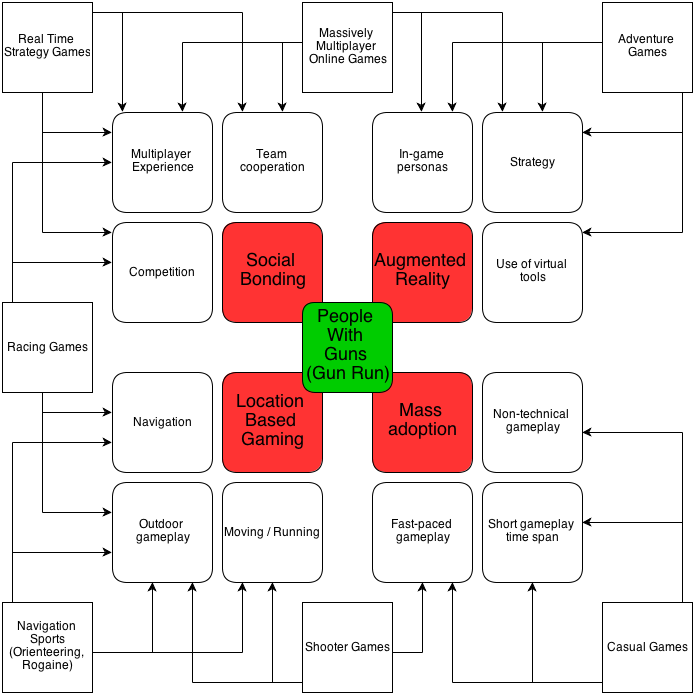
\includegraphics[height=6in,width=6in]{./images/diagrams/ConstructionOfPeopleWithGuns.png}
\caption{\small \sl Conceptual construction of ''People With Guns''(''Gun Run'') 
\label{fig:concept_construction}}
\end{figure}



\subsection{The War Game}

The 'War Game', which has later been named 'People With Guns', is a GPS-based
game in which two teams fight a last-man-standing battle. Each person gets to
choose between a number of character types in the game. How fast one moves in
the game equals how fast one runs in real life.\newline

The player can choose between four types of characters : Medic, Sniper, Scout,
Marine - each with their own specific weapons and health, fitting different
roles within the game.\newline

The rules of the game are simple: two times fight a virtual battle. One team's
purpose is to defeat the opposite team with the means given: each player's real
life movement and the virtual weapons and powerups for fighting. The interface
with the so-called 'weapons' and 'powerups' is layed out in the form of buttons
that are shown on the bottom of the screen. Each weapon or powerup has the
following attributes: range, cooldown, duration, damage. By default weapons have
instant effect(therefore no duration) and powerups have no damage(but they have
a duration) - the only exception is the 'Heal' ability. Both weapons and
cooldowns have a range - an area of effect for their use. If a target falls
within that area, the weapon or powerup of choice can be used. After the
activation of a weapon or powerup, it will be availavbe for use after a time
given by its 'cooldown' attribute. In the case of powerups('Invisibility' and
'Shield'), their time span during which they are in effect after activation will
be given by the 'duration' attribute. \newline

The players are to perform complex communication between each other verbally,
thus maintaining social contact as long as they are in each other's proximity.
For the case of players that are too far away from the rest of their team, a
number of preset messages are provided for quickly exchanging information
between them(such as asking for help, cover or for healing) without distracting
them from the gameplay.\newline

The purpose of this game is to add to the experience of a group of people,
without taking too much focus upon itself. Social bonding and team building are
the goal to be achieved through strategy, tactics and a fun, light game to bring
it all together.\newline

While sliding away from the idea of enhancing a tour mobile app, it was observed
that there are no location-based Real Time Strategy games in existence, or at
least not visible to the thorough search performed to find any.\newline

Based on the previous ideas and some concepts provided into a few games or game
ideas such as Warfinger GPS, MobileWar and racing and navigation games, three
game ideas have been crystalized.\newline 

The games proposed for this project have been :
\begin{enumerate}	
	\item \textbf{Territory Takeover}
	\item \textbf{The War Game}
	\item \textbf{The Mine Game}
\end{enumerate}

1. The \textbf{Territory Takeover} game is a multiplayer, team versus team
competitive game. The players or game author define an area of play, which will
be automatically divided into multiple areas defined by a grid. Each division
will be marked by a 'flag' (a GPS marker). To capture the area division, a team
must capture its flag. The game ends when all flags have been captured and the
winner is the team with most captured flags. Each flag may be given a time that
a player must spend next to it in order to capture it. Once a flag (and
implicitly the territory) is captured, it remains so until the end of the game.
The winner can be decided on flag counting or, alternatively, each flag may
receive a number of points, according to the size of the territory marked by it
and the difficulty of the terrain. \newline

This game can be enhanced with the use of virtual tools or weapons. For the
purpose of this project, the following tools/weapons have been considered :
\begin{enumerate}
	
	\item The \textbf{blocker} is an ability that can be used by each player to
	block an opponent from moving. The 'attacker' 'activates' the ability and a
	circle around him is drawn to show the range in which he can shoot. If an
	opponent enters the range area, the 'attacker' will select him on the map and
	shoot. The 'victim' will receive a notification that he is immobilized. A
	circle or rectangle will be defined around him and he will not be allowed to
	move outside of it for a given time, say 30 seconds or 1 minute. If he does, he
	gets disqualified and kicked out of the game. An alternate solution would be
	that the team loses points, for the case that this is the scoring methodology
	implemented.
	 
	\item \textbf{unblocker} is an ability that an immobilized player can use.
	For this project, it will only work on the person that uses the ability. The
	effect is that a person that is immobilized gets the waiting time halved.
	
\end{enumerate}
Both the abilities have a common cooldown timer. That means that if a player
immobilizes somebody and is immediately immoblized himself, he won't be able to
use the unblocker because of the cooldown following the usage of the
blocker.\newline

For time and effort reasons, this game will not be implemented now, but kept as
future work: it can be added as an extra game type within the app in
development.\newline

2. \textbf{The War Game} is inspired by Real Time Strategy and Shooter games.
Two teams are formed. The area of play may be limited or unlimited. Each
player can choose between a number of characters. The first proposal has been
for four character types: Defender, Marine, Sniper and Heavy Trooper. Each of
the four characters has special abilities and characteristics :
\begin{enumerate}
	
	\item The \textbf{Defender} has the ability to generate shields for short
	periods of time. Members of the team can hide behind those shields for defence.
	The Defender may also act as a Medic and heal or revive members of the team. He
	has low health, long ability cooldowns and a sidearm with short range, small
	damage and fast cooldowns .
	
	\item The \textbf{Marine} has a weapon that can shoot a medium range with
	medium damage and fast cooldowns. He has medium health. 
	
	\item The \textbf{Sniper} has two weapons : the sniper rifle that can shoot at
	distant ranges and deal large damage to single targets and the sidearm, which
	is the same as the Defender's. His health is low, just like the Defender's. The
	sniper shot may penetrate the Defender's shield and cause reduced damage to one
	target.	
	
	\item The \textbf{Heavy Trooper} has three weapons : the bazooka, the sidearm
	and mines. The bazooka is a mid-range weapon with splash damage - it therefore
	can be fired against compact groups, such as the ones that might be hiding
	behind a shield. The bazooka cannot deal damage through the shield, but it may
	be shot next to it, causing damage from the side. The damage to each target
	varies from moderate to small, depending how far they are from the center of
	the 'projectile explosion'. The mines can be placed randomly on the map and
	their 'explosions' will not affect the members of the Heavy Trooper's team.
	Also they cannot be triggered by the members of his team. The damage dealt will
	be moderate, with splash damage, just like the bazooka projectile. The bazooka
	and the mines have long cooldowns, therefore the sidearm is added. The Heavy
	Trooper has high health.
	 
\end{enumerate}


3. \textbf{The Mine Game} is inspired by the classical game Minesweeper,
Warfinger GPS and running games such as the ones in Tourality. It is essentially
a single player game that can be played by many for score ranking. It may be
adapted in various ways directly into the 'War Game'. The purpose of the game is
that the player uses his phone as a mine detector and defuser and navigates
through a virtual mine field, racing against time to get from a start point to
an end point. A variant of this game could be of a team helping a designated
player navigate through the mine field without touching any mines.\newline

Some advantages and drawbacks can be highlighted for these games:\newline

\textbf{Advantages}: They don't require specialized gear and setting, nor
do they need long amounts of time to be played. They can be enjoyed with a
bunch of friends on a sunny weekend afternoon.\newline
\textbf{Drawbacks}: They highly depend on GPS accuracy. This issue may
affect gameplay. This applies especially to the 'Mine Game', which would need
pinpoint accuracy most of the time. \newline

The similarity of the construction of the three above-mentioned games would
allow us to use a common framework that will enable multiplayer interaction for
both 'free for all'/'skirmish' and 'team versus team' approaches and permit the
implementation of the 'Mine Game' along with the others. They would require a
server to centralize player information such as GPS data and various attributes.
Because the games proposed are fast-paced, they require quick response times
from the server, client and and the use of a fast and reliable protocol between
them.\newline

The games are proposed with group teambuilding and recreation in mind. They
require team strategy and cooperation. Territory Takeover allows for both team
versus team and free for all gameplay, allowing for both small and large groups
to play. The War Game is to be a fast paced game spanning a time interval in the
range of a few tens of minutes. Although it contains some Shooter elements -
such as the act of shooting itself - it focuses on strategy and tactics. Quick
reflexes might be required to shoot, but not to aim Where it lacks the realism
of simulations or the immersion of classical computer Real Time Strategy games,
it gains in the intensity of real-life experience and teamwork, without requiring
specialized equipment or highly developed skills. Therefore, the game that is
about to be developed fills a niche between casual and immersive games, bringing
focus to social interaction.\newline

From these three games, the one that was chosen for implementation was 'The War
Game', because it offers a more versatile gameplay, conceptually permitting
a larger number of players, while imposing less time and space restrictions.


\subsubsection{Implementation}

Implementation will mean developing a server and a client application from
scratch, covering all the functionality needed for the main game - the so-called
'War Game' to work according to its description.

\subsubsection{Schedule}
This project, consisting of one server and one client application, was planned
to be developed in four steps:


\begin{enumerate}
  \item \textbf{Development} - During the first iteration of development, the
  most basic features of the game are to be implemented: basic server
  functionality that would allow the game to work, basic client functionality
  and the 'War Game' without all features.(2 months)
  
  \item \textbf{Testing and Evaluation} - During this phase, the game and its
  functionality will be livetested for feasibility and quality. New ideas will
  be sought and documented. Most importantly, player feedback will be
  gathered.(1 month)
  
  \item \textbf{Development} - During the second iteration of development, the
  'War Game' will be completed and, using its framework, the 'Territory
  Takeover' game will be implemented. Bugs will be removed and tweaks will be
  made to the framework and the game concepts to match the player feedback.(2
  months)
  
  \item \textbf{Evaluation and Completion} - During the second evaluation phase,
  both games will be tested for playability, player feedback will be gathered
  and the Dissertation Paper will be completed.(1 month)
    
\end{enumerate}



\subsection{Gameplay}

The gameplay will be presented as a typical scenario of interacting with the
application:

\begin{enumerate}
  \item First of all, in order to get in the game, the player must connect to
  the server. Because this version of the game was created for testing purposes
  only, the server can only host one game. Once there is somebody playing,
  nobody else can join the game. A few seconds after everyone has left the game
  (gone back to the Main Menu), the server will reset itself and accept clients
  once more.
  
  \item Second, once the player has connected to the server, he will be
  presented with the Game Lobby. This is where he joins a team, sets his
  nickname and chooses his character type.

  \item Third, after the player has finished setting up, he can mark himself as
  'Ready' to play the game. If all the players are Ready, the server will send a
  five second countdown and send the signal to enter the game - at which point,
  all connected clients will switch to the game screen and the players can
  start playing.
  
  \item Once in the game, the player's weapons will be enabled only when the
  teams satisfy the starting condition - for now, that means that the average
  positions of all the members of the two teams must be at least 150m apart and
  the members of each team must be at most 20m away from the center position of
  their team.
 
\end{enumerate}

The strategy of the teams can vary and will be more succesful when they devise
one in which they help and back each other, by complementing their skills. That
is why this game can provide both easy, fun gameplay and serious and complicated
strategies, based on the intention of the people playing. Different combinations
of players in each team, according to the needs and style of each player are
possible - and they lead to ever-different approaches in the game.\newline

The game ends when one of the teams is eliminated. Each player's 'character' or
'profession' has a number of associated health points. When the number of health
points reaches zero, the player is eliminated from the game and shown a dialog
giving the options to either quit the game or spectate.\newline


\section{Architecture}

In this chapter we will detail the back end and front end aspects of the game:
how the server and the client are structured, what makes them tick and how they
communicate. We will first analyze the inner workings of the server, then those
of the client and thereafter present the communication in between.\newline

\subsection{Server}


The server was designed for relaying the information in between clients,
centralizing and managing game information - such as keeping track of the teams
and connected players. It is responsible for signalling the clients when to
enter the game and when to start playing. The first signal tells the clients
when to show the game screen and the second one tells them when to enable the
game controls.\newline

Among its roles are managing connections and resending messages - this means
receiving updates from a single client and then unicasting, multicasting or
broadcasting them. All this is done via TCP.\newline

\subsubsection{Managing connections}

For each incoming connection, the server first checks if the game is
in progress (because it is a prototype, the server only hosts one game). If
the game is indeed in progress, the incoming connection is refused. Otherwise,
it is accepted. The server holds a dictionary of connections.
The keys if the dictionary are the IP address : port pairs in the form of
InetSocketAddress object instances specific to each connection. The values
are the unique IDs of the players.\newline

Along the stages of development, connection management has been done as '1
player = 1 IP address', then '1 player = 1 IP:port pair' and ultimately as '1
player = 1 ID'. The first approach could not work for players attempting to join
the game from a subnet. The second approach created some player duplication
issues that have finally been solved with the third. This detail servers to
clarify the next detail in the process of accepting the new incoming connection:
The player connecting to the server sends a 'hello' message with his ID. If he
has no ID, he sends 'null' in the message - and the server generates a new ID
for him. In the case that the player already has an ID, the server will check if
that ID isn't already connected. If it is, the previous connection is closed and
the new one is accepted. Then, the server will confirm the ID or provide it
through the 'configuration' message - which also gives information about the
weapons, powerups and information on the players who are already connected to
the server. Once this is done, a MessageSender and a MessageReceiver object are
created and registered in specific lists. The MessageReceiver object is created
to interpret messages coming from the client and distribute them according to a
message type system. The messages can be forwarded either to the MessageSender
object, or updates entries for the HeartbeatListener - which manages all
connections. The MessageSender relays messages or constructs responses for
requests. The HeartbeatListener is an object that runs a loop and keeps a
dictionary of InetSocketAddress keys with Time objects as values. The loop
periodically checks the dictionary for signs of stale connections. If the record
for a given connection has not been updated in an interval which spans a number
of seconds, the connection is closed.\newline

By closing the connection, we mean closing the inputs and outputs of the
communication socket, removing all communication objects and connection
record and ultimately the heartbeat records.\newline

The connection lifecycle is depicted in Figure \ref{fig:connectionLifecycle}.

\begin{figure}
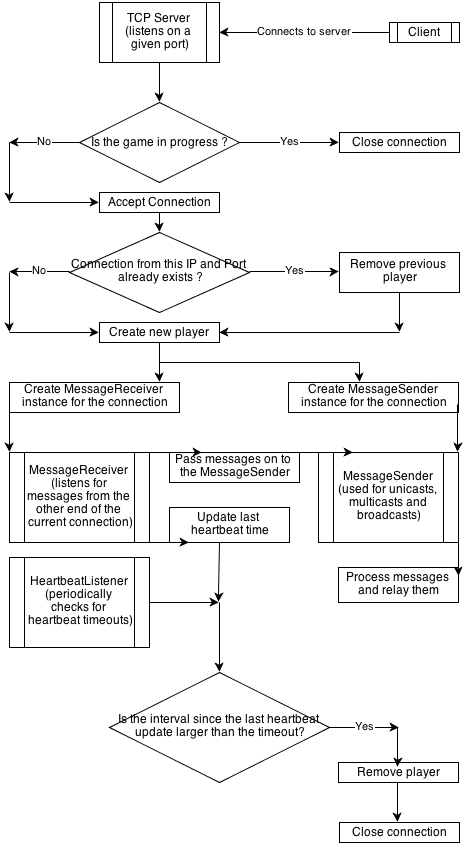
\includegraphics[height=9.00in,width=5.00in]{./images/diagrams/connection_lifecycle.png}  
\caption{\small \sl Connection lifecycle \label{fig:connectionLifecycle}}
\end{figure}

\subsubsection{Relaying messages}

The server acts as a relay, in order to lower the bandwidth and
resource consumption on the mobile clients. The messages exchanged are in
JSON format and have the following base structure: \{messageType: messageNumber,
data: \{\}\}. There are three types of messages, according to the purpose of
their usage: Administration, Lobby and In-game messages. Each of these types has
two subtypes: From Server and To Server. The server replies to or relays what
comes to other clients, according to the specifics of the messages. To this
end, the MessageReceiver checks which type the message is and if it is the case, extracts
data or sends it to the MessageSender. The MessageSender will then construct a
new message or add further fields to the existing one - for example, the
Universally Unique Identifier(UUID) of the sender. Then, according to the type
of message, it will be sent as unicast, multicast or broadcast. The unicast is
sent via the designated MessageSender. Multicasts and broadcasts are sent as
unicasts through many or all the MessageSenders available. Multicasts are, for
now, useful just for in-game messages - teams communicate within. Broadcasts are
used for most types of messages - such as position updates.\newline

\subsection{Client}

The client is the mobile application. It now works with Android versions from
2.3 up. It is structured in six modules, as seen in Figure \ref{fig:clientModules}:

\begin{figure}
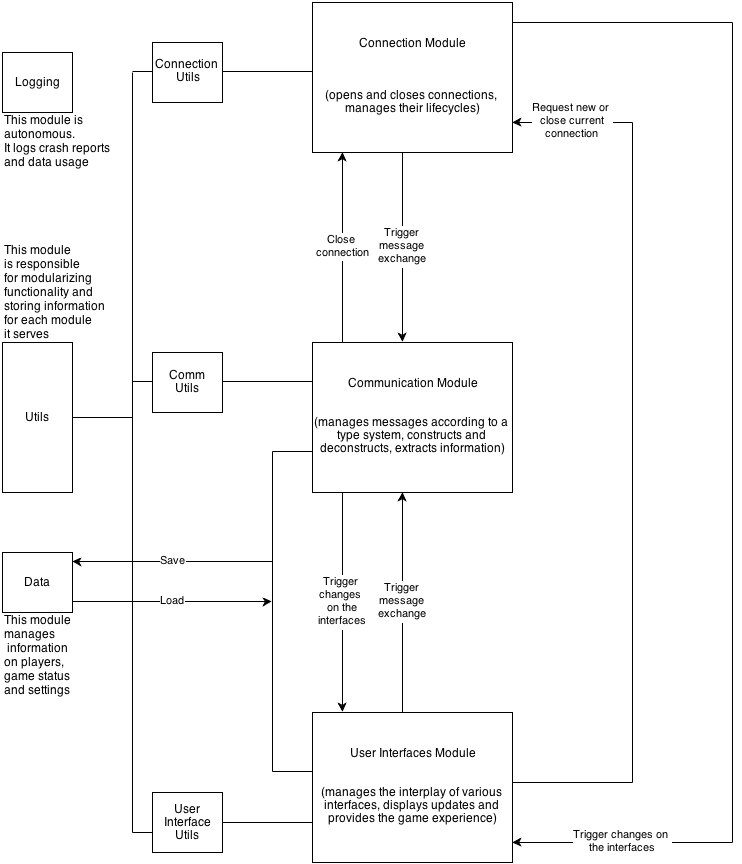
\includegraphics[height=7.25in,width=6.23in]{./images/diagrams/gunrun_module_relationships_3.png}
\caption{\small \sl The Client modules and the
relationships between them 
\label{fig:clientModules}}
\end{figure}

\begin{enumerate}
  \item \textbf{Connection} is responsible with managing the connections:
  starting, stopping and keeping them alive. Implicitly, it works with the
  Communication module, starting and closing the Receiver and Sender objects.
  
  \item \textbf{Communication} is responsible with receiving and
  sending messages. This implies parsing, constructing,
  interpreting, classifying messages.The messages that are to be treated are
  numbered and organized by their purpose or context, according to the
  description already given above.
  
  \item \textbf{User Interfaces} is the module that manages everything
  visual. Each screen in the UI has behind it a Fragment object. They are
  structured by purpose and interlinked. 
  
  \item \textbf{Utils} are the helper classes that provide generic methods.
  Several classes aid various aspects of the functionality of all three main
  modules: Connection, Communication and User Interfaces. For example, they are
  used to keep game state, perform various checks and activate or deactivate
  controls on the User Interfaces.
  
  \item \textbf{Storage} is composed of static classes holding
  information about the players in the game, their status, available professions
  and weapons. Also safe access to the data is provided through methods present
  in these classes. Storage also provides functionality to save data for the
  next run of the application - such as the IP and port of the server or the
  last used nickname and character type of the player. 
  
  \item \textbf{Logging} contains the Logger class, which can be used to log
  anything that would be important to be analyzed. For now, the logging module
  is responsible for storing crash dumps and data usage information in files.
\end{enumerate}

The UI of the client app is split into the 7 fragments presented under 'User
Interfaces' in Figure \ref{fig:clientModules}. When the app is run, the first
screen is the main menu. A check will be made if the prerequisites for
playing the game are met(having Google Play Services installed and the
GPS turned on). If either one is not met, a dialog will help the player
quickly get the Google Play Services or turn on the GPS. Buttons in the main
menu provide navigation to the main menu settings, tutorials or lobby(provided
there is an Internet connection). The tutorials work offline and provide some
insight on what the game is and how it is played. The settings screen is a
temporary solution for manually giving the IP address and port of the server to
which the client is to connect. The 'Connect to server' button triggers a
connection attempt. A loading screen will be briefly presented while work is
done in the background. In this case, the connection is established and 'hello'
and 'configuration' messages are exchanged by the server and client. Once this
is done, the loading screen is replaced by the Lobby screen. Here, the player
can choose between teams and edit his character details via the LobbySettings
screen. Once this is also done, the player will signal the fact that he is ready
via the 'Ready' button available on the screen. If all players are ready, the
server will send a countdown, followed by a message signalling game entry. This
is when the Lobby screen is replaced by the Game screen. The whole game UI is
available at this time, with the exception of the weapon buttons. At this point,
the server will make a check on whether the teams are far enough from each
other. When the teams get far enough from each other, the server will send the
signal to start the game. This is when the game buttons are enabled and the
virtual battle begins. The two teams will attempt to eliminate each other
through the use of virtual weapons and powerups, and strategy.\newline


\begin{figure}
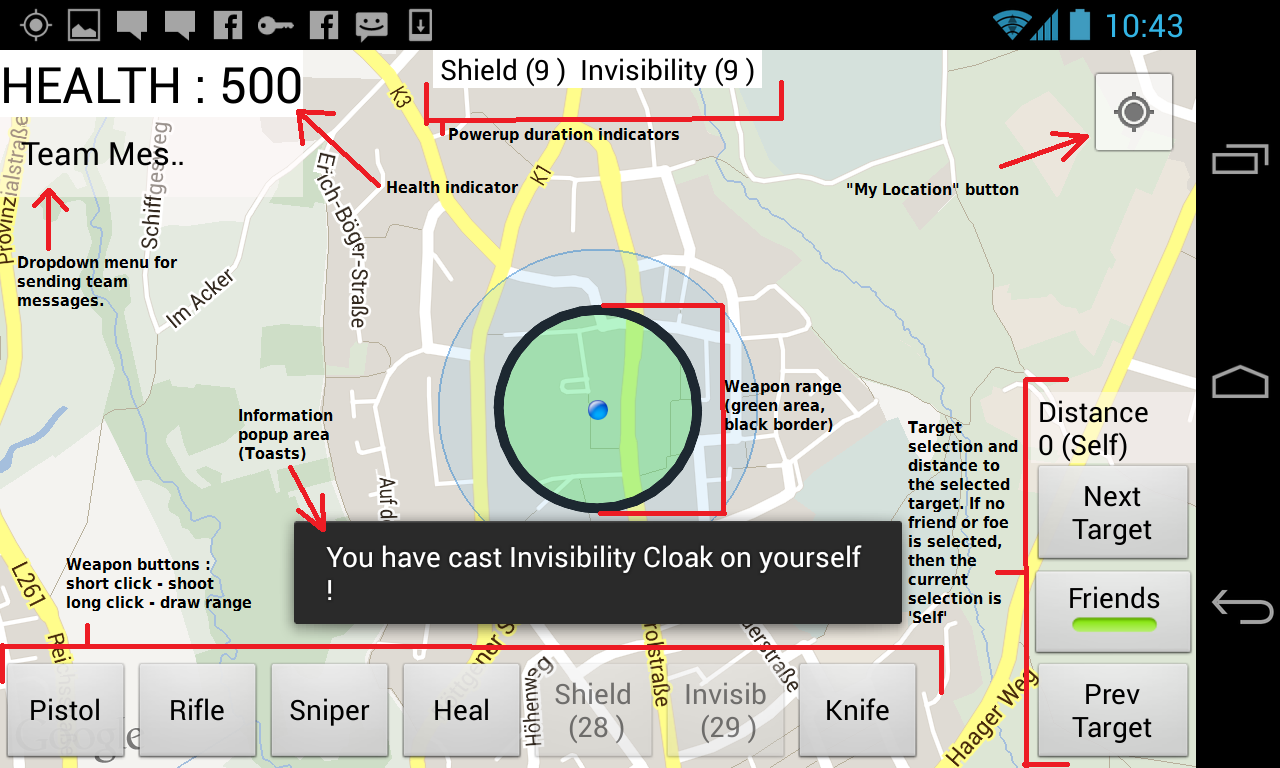
\includegraphics[height=3.5in,width=6.23in]{./images/android_screenshots/tutorial_game.png}  
\caption{\small \sl The in-game UI \label{fig:game_ui}}
\end{figure}


The in-game controls are separated in six areas, as seen in Figure\ref{fig:game_ui}:

\begin{enumerate}
  \item \textbf{The bottom area}: the Weapons: For each weapon there is a
  separate button. Each button serves three purposes: If the player presses it,
  the weapon or power-up linked to that button will shoot. If the player presses
  a weapon button for a longer time, the range of the weapon will be drawn on
  the map. Once a weapon was successfully used(on a target within its range),
  the button will be temporarily disabled and will show the weapon cooldown
  countdown.
  
  \item \textbf{The down-right corner}: The target selection buttons: The player
  can select his targets (both friends and enemies) by clicking on their
  markers on the map. As an alternative, three buttons are there to help him:
  the Friends/Enemies toggle button, with which he can choose from which
  group the selection will be made: friends or enemies. Above and below the
  toggle button are the 'Next Target' and 'Prev Target'(Previous Target)
  buttons. By pressing the 'Next Target' button, he will select the next closest
  player(If there is one selected, the next closest one will be chosen. If
  nobody is selected, the closest one will be chosen.). The 'Prev Target' button
  gets the opposite: the previous farthest friend or foe is selected, according
  to the same logic as with 'Next Target'. Above the three buttons, he can find
  a text view which shows the distance to the selected target. By clicking a
  random empty area on the screen, he will deselect whichever player was
  selected. Having no one on the screen selected is equal to having oneself
  selected - this is necessary for using power-ups on oneself.
  
  \item \textbf{The top-left corner}: The health and messages buttons: The
  player's health is shown in large font. Below it, he can find the message
  selection dropdown menu. This has been arranged so that he does not waste time
  typing, but instead send critical preset messages to his team, when verbal
  communication is not possible.
  
  \item \textbf{The top-right corner}: The current position button: If the
  player presses it, the map moves to have your position in the center.
  
  \item \textbf{The top-center area}: The power-up duration views: If the player
  enables a power-up or somebody uses a power-up on him(for now, this applies
  only to the 'Shield' power-up), he will see its remaining duration of the
  effect as a countdown on the top of the screen.
  
  \item \textbf{The area above the weapon buttons}: The information area:
  Whenever the player shoots, is shot, sends or receives a message a 'Toast'
  will appear with info. The 'Toast' is an Android-specific short message that
  appears on the screen for a short time.
  
\end{enumerate}


\subsection{Communication}

Communication in between client and server is done via TCP connections that are
kept alive all along the game. The server manages a separate connection with
every client. The messages are in the JSON format and are serialized and
deserialized with the Jackson library.\newline

For each connection, the server creates a MessageSender and a MessageReceiver
objects, each acting autonomously - their lifecycle is managed by the server.
The Receiver has more responsibility, as it can close the entire connection
or call the MessageSender(or a subset of all the MessageSenders associated with
the connected clients, in the case of a broadcast or multicast) to deliver
messages.\newline

In addition to the Sender and Receiver objects, a 'heartbeat monitor' object is
running in the background and checking the liveness of all the connections. A
client sends periodic heartbeat messages to show that it is still alive. The
'heartbeat monitor' is responsible for closing the connections that have not
sent a heartbeat update in a given time frame - 3,5,10 and 15 second frames have
been tried out.\newline

As previously presented, all messages have the following JSON structure:
\{messageType: messageNumber, data: \{\}\}. We are now interested in the data
structure. The messageType is a number that both client and server recognize(as
the Messages class is present in both client and server). Both Server
and Client, when they receive a message, peel the structure layer by
layer and extract information. In the case of the Server, it sometimes
only extracts the messageType, adds a parameter such as the ID of the
sender and relays it. The structures of two messages are presented in
contrast in Figure\ref{fig:message_structures}: The Configuration message,
which is the most complex one, and the Shoot message, which is much lighter.\newline

\begin{figure}
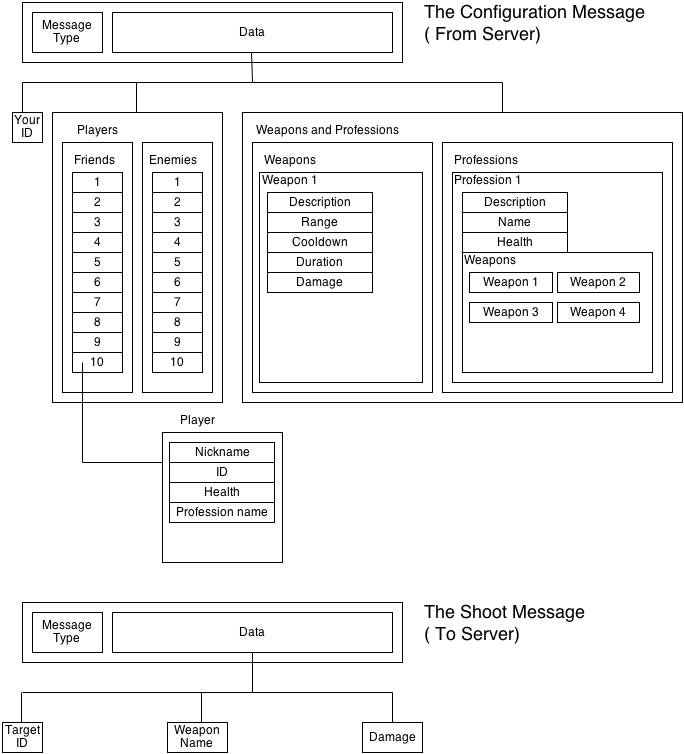
\includegraphics[height=6.6in,width=6in]{./images/diagrams/message_structures.png}
\caption{\small \sl The structure of two of the messages exchanged by the Client
and Server
\label{fig:message_structures}}
\end{figure}

The Server is active in the message exchange only for the basic administration
purposes: Once a player connects, he receives a configuration json containing
the available 'weapons', 'professions' (with all their attributes) and the list
of already-connected players. It also broadcasts a message telling the existing
players that a new player has connected. When a player disconnects or is
disconnected from the server, a message telling the others that he is
disconnected is sent automatically by the server. Otherwise, the server acts as
a relay.\newline

The Messages class contains a number of inner classes, for proper
classification. We will present the structure, the message types and their
specific JSON structures within:

\begin{enumerate}
  \item \textbf{InGame.ToServer}  
  \begin{enumerate}
    \item CHANGE\_POSITION :
    \{latitude: newLatitude, longitude: newLongitude\}
    
    \item SHOOT :
    \{target: targetUUID, weapon: weaponName, (optional)timestamp: timeStamp\}
        
    \item MESSAGE\_TEAM :
    \{message : messageString\}
      
  \end{enumerate}  
  
  \item \textbf{InGame.FromServer}  
  \begin{enumerate}
    \item CHANGE\_POSITION :
    \{player: playerUUID, latitude: newLatitude, longitude: newLongitude\}
    
    \item SHOOT :
    \{player: playerUUID, target: targetUUID, weapon: weaponName, damage:    
    damageAmount, (optional)timestamp: timeStamp\}
    
    \item MESSAGE\_TEAM :
    \{player: playerUUID, message: newMessage\}
    
    \item GAME\_START :
    \{\} 
        
  \end{enumerate}  
  
  \item \textbf{Lobby.ToServer}
  
  \begin{enumerate}
    
    \item MESSAGE\_ALL :
    \{message: messageString\}
    
	\item CHANGE\_NAME :
	\{name: newName\}
			
	\item CHANGE\_TEAM :
	\{\}		
	
	\item CHANGE\_PROFESSION :
	\{profession: newProfession\}
	
	\item CHOOSE\_WEAPONS :
	this will be made available in further versions where there will be more
	weapons from which to choose
	
	\item READY :
	\{ready : true/false\}    
     
  \end{enumerate}
  
  
  \item \textbf{Lobby.FromServer}
  
  \begin{enumerate}
    	\item ENTER\_GAME :
    	\{\}
		
		\item MESSAGE\_ALL :
		\{player: playerUUID, message: messageString\}
		
		\item CHANGE\_NAME :
		\{player: playerUUID, nickname: newName\}
		
		\item CHANGE\_TEAM :
		\{player: playerUUID, team: newTeam\}
				
		\item CHANGE\_PROFESSION :
		\{player: playerUUID, profession: newProfession\}
		
		\item READY :
		\{player: playerUUID\}
										
		\item PLAYER\_JOINED :
		\{player: playerUUID, name: playerName\}
		
		\item PLAYER\_LEFT :
		\{player: playerUUID\}
			
		\item CONFIGURATION :
		A huge JSON thing that the Server composes based on a configuration file and
		sends it to the client. 
		
		\item COUNTDOWN :
		\{secondsLeft: numberOfSecondsLeft\}
		
  \end{enumerate}  
  
\end{enumerate}

The flow that is triggered by a new client connecting to the server is
presented in Figure\ref{fig:client_server_flow}. The flow triggered bt an existing client leaving the
server is presented in Figure\ref{fig:player_disconnected}.

\begin{figure}
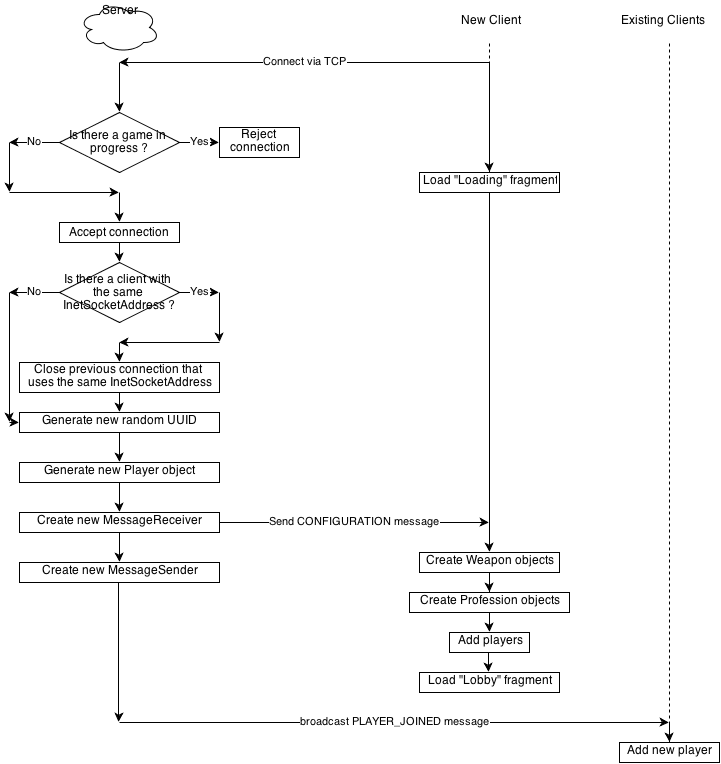
\includegraphics[height=7.665in,width=6.23in]{./images/diagrams/Client-Server.png}
\caption{\small \sl A new client joining the game
\label{fig:client_server_flow}}
\end{figure}

\begin{figure}
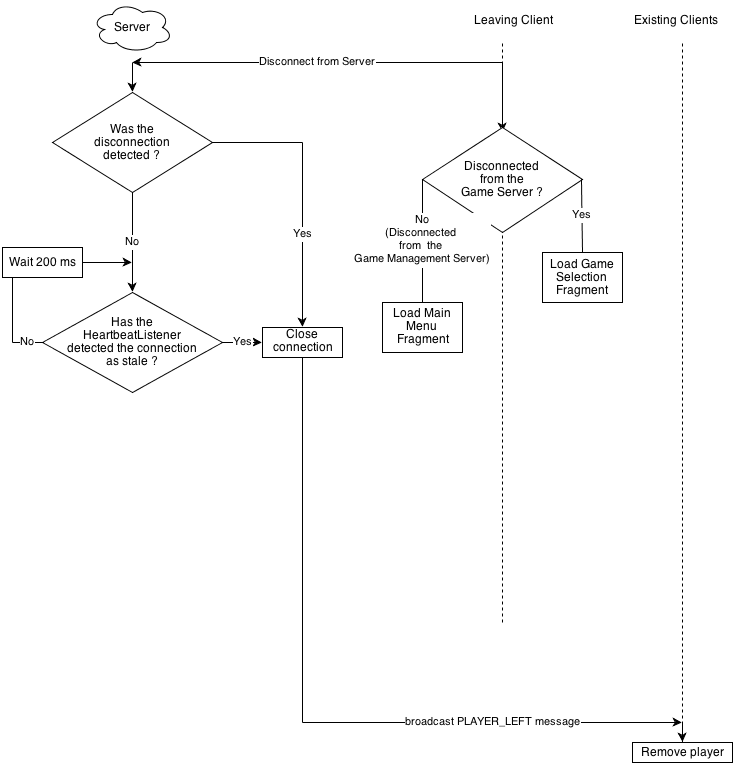
\includegraphics[height=7.665in,width=6.23in]{./images/diagrams/player_disconnected.png}
\caption{\small \sl A client leaving the game
\label{fig:player_disconnected}}
\end{figure}


\section{Development timeline}

This section will follow the conceptualization and implementation of
the game ''People With Guns''. The back end and mechanics of the game will be
analyzed and presented in their evolution, also briefly describing aspects of
the front end. \newline

In this chapter, we will see the steps taken until the idea for the game has
been crystalized. Then, we will follow the steps of development and field
testing of the server and client, chronologically.


\subsection{The exploration phase}

The development of the app has started on the 14th of January 2013.
The evolutionary steps and intermediary and final concepts are presented here.\newline

\subsubsection{Creating the game concept}

The project had started as a proposal to add a multiplayer feature to a tour
app. Simply adding the functionality to see all the others within the group on
the map was not sufficient - it would just help if someone got lost or went
astray. Otherwise, it was concluded that the user experience would not be
improved in any significant way. Then came the idea of adding small games,
hidden caches or quests and so on. The best idea that still had the tour app as
a main platform was to add detours from the main track as bonuses. On those
detours, the people would have to solve various riddles and small puzzles to get
points and find out about hidden historical spots or interesting facs about the
places they are visiting. \newline

At this point, the following addon to the main app was contoured: the
players would have a main tour path and, as they passed by certain waypoints,
would be offered to go through a bonus/extra track within the area that they are
visiting. If enough of them would agree to do this(by an in-app vote, for
example), they would be presented with a new set of waypoints. These waypoints
would belong to a number of categories: normal waypoints, waypoints where they
would have to split, waypoints where they would have to be together and
waypoints where the whole group would have to wait within a virtual circle,
while one delegate(through vote) would find an item or solve a riddle -
of course, with the help of the entire group.\newline

Another scenario has been proposed, during the research: In the case of the
group waiting and one member being delegated to solve a riddle or find an item,
a means of cooperation can be brought up: When the team votes and chooses the
delegate, his screen turns black(no map) and the rest of the team can see
the goal on their phones. Through messages or in-app voice communication,
they would help the delegate navigate to the goal. Then, once the goal has been
found or reached, the virtual circle would disappear and the whole team would be
free to move. If anyone would exit the circle at some point, they would receive
penalties and eventually get disconnected from the game.\newline

Gradually, the ideas for multiplayer features went astray from the tour app,
towards multiplayer GPS-based games. The idea of GPS-based puzzle / adventure
games was explored ARIS was encountered - a platform for creating such games.
Then Tourality was discovered, and WarFinger GPS, which have been the main
sources of inspiration for the 'War Game' and a few other games that didn't make
it in the main concept, but are to be developed within the game as future
work.\newline

There has been a point when all the GPS-based mobile games that could be
found were studied and where possible, played. Then they were evaluated for
advantages, disadvantages and gameplay. At this point, the goals for the game to
be developed were already in mind: It should move the players to an outdoor
environment and have them walk and run as the main activity, while using the
game itself for an improved experience. Hide and seek and Tag were considered as
a model of entertaining game to be played by a group. The games found and
already enumerated can be considered to have one of two major disadvantages:

\begin{enumerate}
  \item Do not engage the users enough: Games such as Parallel Mafia, SCVNGR or
  Please Stay Calm do not motivate the player to move around much. They also
  offer a very dim user experience in areas with few or no players.
  \item Engaged the users too much: Mobile users, even hardcore gamers, do not
  spend too much time playing on the phone. Rather, they would play on consoles
  or computers, for better immersion. No matter how good the game is, it is
  still displayed on a small phone screen(tablets are not considered in this
  paper). Games such as Ingress and Shadow Cities offer a better and more
  immersive story, but are still demanding of the player and request the full
  focus of the phone owner. This can be considered as a major downside, as at
  least some people(the author included), do not want to be engaged for
  prolonged amounts of time, nor to deviate from their usual trips through
  the city for the sake of a game, nor will they spare the time and will to play
  such a demanding game while on the go.  
  \item Do not motivate the players to move enough - Only Tourality does not
  possess this downside, as it its various game modes are specifically designed
  for running.
  \item Are location-dependent - All adventure / puzzle games such as those
  developed with ARIS, most MMOs such as Parallel Mafia do require the player to
  be in certain places in order to progress through the game. This means that
  the player is put in one of two situations : he 1. has to get out of
  his way in order to make any progress within the game, or 2. has to travel
  to remote locations in order to play the game in the first place. This might
  be interesting for some, but does not cover a broad spectrum of population. 
\end{enumerate}

The engagement problem can also be linked to a time problem. Games that are
highly engaging also require a lot of time to be played. The arugment that the
amount of time dedicated to the mobile game should be decided by the player and
not by the game has been used in the construction of the concept of the game
that was eventually developed. \newline

\subsubsection{The game concept}
The app developed is temporarily called ''People With Guns''. It is a GPS-based
Real Time Tactics game with Shooter elements, developed for Android. It can be
played by several people (The upper limit has not been established yet. Until
now, the highest number of players in the game has been six) that choose to join
one of the two opposing teams. The purpose of the game is to use 'weapons' and
'powerups' to defeat the opposing team. By 'defeat', we mean to use the
available tools provided by the game to reduce the virtual 'health' attribute of
all the opponents to zero.\newline

The current 'tools' are as follows :\newline

The weapons : 
\begin{enumerate}
  \item Pistol
  \item Rifle
  \item Sniper Rifle
  \item Knife   
\end{enumerate}

The 'powerups' :
\begin{enumerate}
  \item Invisiblity Cloak
  \item Shield
  \item Painkillers / Heal
\end{enumerate}

Each item used by a player has the following attributes : 
\begin{enumerate}
  \item Cooldown - The amount of time that has to pass until the weapon can be
  used again.
  \item Duration - The amount of time during which a powerup is in effect 
  \item Damage - The amount of health points that are subtracted upon a hit (or
  added, in the case of the Painkillers / Heal ability) from the target's total
  available health points.
  \item Range - The maximum distance within which a weapon can be fired.
\end{enumerate}

The difference between weapons and powerups is that the weapons are the
principal means of winning the battle, while the powerups are helpers to either
keep the players present in the game for a longer time. Weapons are offensive,
while powerups are defensive.\newline

Another differentiation between weapons and powerups can be made based on their
attributes. Until this point of the game development, weapons have damage and no
duration. The only powerup that also has damage are the Painkillers, which
'heal' the target (they deal negative damage to it). The other two powerups,
Invisibility Cloak and Shield, have a greater than zero 'duration' attribute,
but no 'damage'.\newline

Some of the attributes of the weapons and powerups will be modified, during
several phases of balancing. Therefore, only their conceptual construction will
be described, without numbers:

The weapons : 
\begin{enumerate}
  \item Pistol - Weapon with low damage and medium fire rate. All the character
  types have it. It is the basic and least effective weapon of them all. The
  range is small.
  
  \item Rifle - Weapon with low damage and high fire rate. The damage is higher
  than that of the pistol and the cooldown takes much less. The range is small.
  
  \item Sniper Rifle - High damage weapon with very low fire rate. The range is
  far greater than that of the Rifle and Pistol.
  
  \item Knife - The weapon that deals the highest damage of all. The cooldown is
  greater than that of the Sniper Rifle and the range is very small.
   
  \item Invisiblity Cloak - Powerup that makes the player disappear from the
  map for a short while. While the player is invisible, he cannot be shot.
  The effect duration is short, while the cooldown is lengthy.
  
  \item Shield - Powerup that, while it's in effect, reduces the damage taken to
  half. The duration of this powerup is short and the cooldown is lenghty.
  
  \item Painkillers / Heal - Powerup that restores a large number of
  health points to the player or his friends. It has no duration - just like
  a weapon, it's effect is applied immediately. It requires a lengthy cooldown
  time.
  
\end{enumerate}

For more complexity in the game, a number of so-called 'character types' have
been created, from which players can choose. Thus far, there are four character
types implemented in the game: Marine, Medic, Sniper, Scout. Each of these has a
different number of health points and different weapons. Because several
character balancing phases are on schedule, only the conceptual construction of
the characters will be mentioned, without numbers :

\begin{enumerate}
  \item Marine - Has average health and two weapons: Pistol and Rifle.
  Represents the basic attack unit.
  
  \item Medic - Support unit with Shield and Painkillers/Heal abilities. Has
  high health.
   
  \item Sniper - Attack/ defense unit. Has a Sniper Rilfe for shooting at large
  distances. Has average health.
  
  \item Scout - Attack unit specialized at sneaking up on the victim. Has the
  'Invisibility Cloak' ability for disappearing from the map and the 'Knife'
  weapon for dealing large amounts of damage within a very small range. Has
  small health.
  
\end{enumerate}

Another character has been created for testing purposes. It has been called the
'All Encompassing' and posesses all the weapons and skills presently existing in
the game and very large health. This character has inadvertently opened a window
for two more game types:

\begin{enumerate}
  \item 'David versus Goliath' - This is proposed to be a game of many players
  using regular character types versus a much smaller number of 'All
  Encompassing' characters.
  
  \item 'Duel' - During the many gameplay of this app, a new style of playing
  this game has emerged: in the absence of a large enough number of players, two
  can play in the 'Duel' mode : both use the 'All Encompassing' character type
  and, instead of moving around, attempt to win the game by optimizing  
  combinations of weapons and powerups. This game is generally played side by
  side, for at most a few minutes and has proved to be entertaining for the ones
  who tried it out.
\end{enumerate}



\subsection{The first development phase}

The first development phase was mainly one of searching for the right
technologies to be used for the development of this game. The functionality
of serveral technologies and combinations of them has been tried out. Once
the decision has been made on which will be used to develop the game, some
prototypes have been made for the server and front end and back end of the
client.\newline

The initial idea has been to use Websockets for communication, a Node.JS server
and, a native Android client. The messages exchanged between server and clients
would be in the JSON or XML format. Based on some brief research, JSON was
chosen - it is easier to use and it takes less bytes to transmit the same data
as it would with XML. The plan has been to use simple data structures for the
messages that were to be exchanged between server and clients. For JSON
serializing and deserializing, the choices found viable were Jackson and
Google GSON. After determining their speed and ease of use Jackson has been
chosen, as besides its speed, it offers an easy way of serializing and
deserializing JSON directly into a hierarchy of HashMaps - peeling down layers
of the JSON - which better serves the relaying of messages of the server side.
\newline

Exploring the use of Websockets has proven unfruitful, as there have been dead
ends :

\begin{enumerate}
  \item The only freely available Websocket library for Android at the time of
  research was Autobahn. The Websocket libraries available for NodeJS were
  Socket.IO, Websocket-Node and ws. None of them worked with Autobahn for
  Android. A forum post was eventually found, in which one of the developers of
  Autobahn stated the reasons for the incompatibility between Socket.IO and
  Autobahn for Android: First, the protocol implementations were based on
  different draft versions. Second, Socket.IO used an HTTP handshake for the
  connection - and that was not supported by Autobahn. The same issue applied to
  Websocket-Node and ws. A Python implementation of Autobahn has been tried for
  the server, but after a few unfruitful attempts, the decision was made to
  use Java. In the case of Java, Autobahn for Android does not work. One of the
  reasons: Autobahn subclasses a Handler object that is part of the Android
  SDK. So it was decided that until Websockets becomes a stable protocol, TCP
  will be used.
  
  \item Because of the Websocket issue, Node.JS development has been perceived
  slow (Libraries are not documented, autocomplete mostly does not work and
  there is no javadoc equivalent), even considering that the author had
  previous experience with it. The decision was made to switch to Java.  
\end{enumerate}

In the end, the technologies used have been native Android for the
client, Java for the server server and TCP communication in between with JSON
messages parsed with Jackson. \newline

As tools were chosen, the development of the app has started.
The beginning of the first phase development has been concerned with creating
three prototypes:

\begin{enumerate}
  \item The design of a game UI prototype that would add some mock players on
  the map and provide usability insight.
  
  \item The design of a game menu prototype.
  
  \item The development of a basic server prototype, without great concern for
  robustness. Its responsibilities would be to manage connections and relay
  messages.
  
\end{enumerate}

In developing the initial game UI, three buttons (one for
generating a number of markers ('Generate Markers') on the map, one for testing
purposes('Check Info') and one for shooting ('Shoot')) and a Spinner were added
on top of a MapView (a map screen). The spinner served as a weapon selector.
Once a weapon was selected its range would be drawn on the map. The three
buttons have been placed in three corners of the screen- bottom-left,
bottom-right, top-left. The spinner has been layed to the right of the 'Shoot'
button. The functionalities added were as followed :

\begin{enumerate}
  \item 'Shoot' button - Mock method to display a Toast message stating if the
  shot was performed or not by the selected weapon.
  
  \item 'Generate Markers' button - Mock method to randomly generate
  player markers on the map.
  
  \item 'Check Info' button - sporadic functionality to display a Toast message
  with various information on data structures in the back end.
  
  \item Spinner - Responsible with weapon selection. 
\end{enumerate}


\subsubsection{The structure of the server}
 
The server has been structured from the beginning in three modules: 

\begin{enumerate}
  
  \item A 'Communication' module for dealing with adding and managing
  connections and messaging.
  
  \item A 'Messages' module for managing the incoming and outgoing messages for
  each connection.
  
  \item A 'Game' module for handling in-game data, such as keeping track of
  connected players, teams and game status. 
  
\end{enumerate}

The structure of the 'Communication' module:

\begin{enumerate}
  
  \item The 'TcpServer' class that manages the server socket loop that is
  listening for incoming TCP connections on a given port.
	
  \item A 'ConnectionManager' class that provides methods for managing
  connections: keeping track of the connected clients, creating MessageSender
  and MessageReceiver objects to serve each client. Part of this
  module is the so-called HeartbeatListener, which periodically checks the
  liveness of connections and closes the stale ones.
  
\end{enumerate}

The structure of the 'Messages' module:

\begin{enumerate}
  
  \item A 'Messages' class that keeps a record of the possible messages between
  client and server, organized into inner classes for ease of use. This class is
  also present on the client.
  
  \item A 'MessageSender' class that deals with sending messages to a single
  client, but can also access all other instances of this class to multicast
  and/or broadcast messages to all the other clients, when needed.
  
  \item A 'MessageReceiver' class that deals with receiving messages from a
  single client.
  
\end{enumerate}

The structure of the 'Game' module:

\begin{enumerate}
  
  \item A 'Player' class that defines which information about the players
  (eg. name, 'profession', health points and position) is to be stored.
  
  \item A 'GameManager' class that manages the addition, removal and management
  of players.
  
\end{enumerate}

\subsubsection{The Server}

Once started, the server listens on a port. When a remote client connects, the
server adds an InetAddress instance containing the IP address of the client.
Then, a Player object with some default values is initialized and a random UUID
is generated.\newline

The Player object is added to one of the two dictionaries that are used for
keeping evidence of the two teams of players - home team or away team - using
the player IDs as keys. A MessageReceiver and a MessageSender are instantiated.
The MessageReceiver and MessageSender are registerd into two dictionaries, one
for each, using the InetAddress of the client as key.\newline

Once the initial management tasks have been done and the new player is fully
registered on the server, the server sends a configuration message containing a
list the already connected players, the available professions and their
attributes(title, health, weapons, description), the available weapons and their
attributes(name, range, cooldown, duration, description and usage
policy).\newline

From now on, whether a player remains connected to the server depends on the
so-called heartbeats: The client will send periodic heartbeat(keep alive)
messages to the server. The server holds evidence of the heartbeats it
receives from each player. On each update receipt, it will update the time of
receipt in a dictionary. If no update has been received in a given amount of
time, the client's connection is deemed stale and closed. \newline

The server now acts only as a relay - game state is held on the client
side.\newline

Because TCP does not allow multicasts and broadcasts, a workaround for sending
multicasts and broadcasts has been devized: When a client sends a message that
requires to be multicast/broadcast, the server accesses all the MessageSender
objects(each one is responsible for sending messages from the server to a
specific client), iterates through all of them and sends the given message to
all of them. This applies to various updates, and in-game messaging.\newline

Once a number of players (1 or more) have connected to the server, they may send
'Ready' messages to the server, signalling that they are prepared to enter the
game. When all the players are ready, the server will broadcast a five second
countdown to all the clients. After the countdown, an 'Enter Game' message is
broadcast. Because the server holds the information on the positions of all the
players, a condition and another message have been added: when the distance
between the centers of the polygons described by the positions of the
team members is at least a number of meters(eg. 500m) and each team member is at
most a number of meters(eg. 50m) away from the center position of his team, a
'Start Game' message is broadcast to all the clients. This will later be used to
enable the weapons for all the players only when they satisfy these
conditions. For now, the condition calculation is done, but the message
is not taken into consideration by the client.\newline

There is no direct disconnect message between server and client, nor is there
any disconnection detection in this phase of development. Disconnection is done
exclusively based on the heartbeat interval.\newline

\subsubsection{The Client}

The client is a native Android application. It uses Fragments for showing
various UI screens. It does not use any compatibility libraries. The Google Map
API V1 is used (as the Google Maps V1 API has some incompatility issues with the
Android Support Libraries that would allow the game to be played on earlier
versions of Android) and therefore, only Android versions equal or higher to
3.0(Honeycomb) are supported.

The client presents seven UI screens to the player: 'Main Menu', 'Info and
Tutorials', 'Settings', 'Lobby','Lobby Settings', 'Loading' and 'Game':

\begin{enumerate}
  \item 'Main Menu' : It is the entry point of the the application (it is the
  fragment loaded when the application is started). It features three buttons:
  'Start Game', 'Settings' and 'Exit'. By pressing 'Start Game', the player
  attempts to join the game. If the connection is successful, he is brought to
  the 'Lobby' screen. Pressing 'Settings' leads to the homonymous screen.
  
  \item 'Settings' allows the player to change the IP addres and port
  number to which the client will attempt to connect.
  
  \item 'Loading' is an intermediary fragment that shows a loading widget
  while, in the background, the connection to the server is established
  and the client receives the configuration data from the server. Once
  this process is done, it automatically switches to the 'Lobby' screen.
  
  \item 'Lobby' is the game preparation screen. It shows the lists of players in
  the two teams and their details(nicknames, professions and 'Ready' status).
  This screen features four buttons: 'Back', 'Change Info', 'Change Team' and
  'Ready'. Pressing the 'Back' button closes the connection and returns the
  the 'Main Menu' screen. By pressing the 'Ready' button, the player toggles
  his/her 'Ready' status and sends a message containing this status to the
  server. The 'Change Info' button switches to the 'Lobby Settings' screen.  
  
  \item 'Lobby Settings' is the screen which allows the player to change his
  nickname and 'profession'/'character type'. It also shows a short description
  of the selected character type, followed by an enumeration of the available
  weapons for that character.
  
  \item 'Game' is the most important screen in this app: it provides the UI
  for gameplay. It features a fullscreen MapView that displays the map and, on
  top of it, the 'Shoot' button and weapon selection Spinner. Two other buttons
  are kept on the screen and given various functionalities, according to the
  testing needs.
   
\end{enumerate}

The typical game usage scenario would go as follows: The player opens the
application and is presented the 'Main Menu' UI. If the GPS is not on, a dialog
will appear informing him of this and offering two choices: `Turn GPS on` or
'Exit' the game. If 'Turn GPS on' is chosen, the GPS Settings page will be shown
and the player can switch it on. Once this is done, the player presses the 
'Start Game' button and, after being briefly shown the 'Loading' screen, is
introduced to the 'Lobby' screen.\newline

Here, one can see that he has been added to one of the teams(Home Team or Away
Team) and has been given a default nickname('Player') and profession('Marine').
This is where he can choose to switch between teams by pressing the 'Change
Team' button. Then, he navigates to the 'Lobby Settings' screen by clicking the
'Change Info' button and change the 'nickname' and 'profession'. Once the player
is ready to play, he will press the 'Ready' button. If all the players that are
connected to the server are marked as 'Ready', the server will send a countdown
(which is seen on the client side through Android-specific Toast messages)
followed by a 'Start Game' message - at which point the client app will
automatically introduce the 'Game' UI. \newline

All the players are shown on the map by blue(current player), red(enemies) and
green(friends) markers. Above each marker, one can see the nickname,
'profession' and health points of the player. The selection of players is done
by clicking the markers. A selected player will have his marker drawn in yellow.
Selecting a weapon from the provided Spinner deselects the currently selected
player(if there is any) and draws the weapon's range around the position of the
current player. For using the currently selected 'weapon' or 'powerup' on one of
the other players, the player has to select the target by tapping its marker on
the screen and press the 'Shoot' button. If the selection attempt does not
satisfy the 'selection policies' provided by the Weapon object, the map marker
will simply not be selected. Otherwise, it will change color to yellow. If the
target is not within the weapon's range when the 'Shoot' button is pressed, a
Toast message will appear stating the distance between the player and his target
and that the shot was not performed. Otherwise, a Toast message showing the
distance and damage dealt will be shown and a cooldown countdown will start at
the appropriate entry of the weapon selection Spinner object. Once a player has
lost all health points, a dialog appears telling him that the game is over for
him and gives him the sole option to exit the game and return to the 'Main
Menu' screen. Once a player exits the game, his marker will disappear from the
maps of the other players. There are no start and end conditions implemented.

\subsubsection{The UI}

The design of the UI has been done progressively, using intuition at the
beginning and player feedback for further improvements. We will now describe the
first interation of UI design.\newline

During the first phase of development two UI prototypes have been created: one
for the game screen and the other for the menus. A rough idea on what the game
will look like and what functionality the UI has to provide was made once the
two UI prototypes were put together and tried out.\newline

We will first discuss the game screen prototype. The first challenge has been
more to create the Overlay object, get markers of four color types (red: enemy,
green: friend, blue: current player, yellow: selected player) on the map at
random positions and create the first 'Shoot' action seem real. This meant
adding a 'Shoot' button and a Spinner from which weapons could be chosen and
adding player selection into account. It had to be realistic, so a list with
Weapon objects had to be created. For this, attributes had to be conceived for
these weapons. The first two attributes attributed to the weapons have
been 'damage' and 'range'. Once this has been done, drawing the range of the
selected weapon on the map became the focus. Once that was done, shooting a
weapon had to give some feedback. That's when Toast notifications have been
added. After this, it was noticed that the weapons can be shot continuously.
They weren't supposed to. The 'cooldown' attribute has been added to the
weapons and the functionality to run a countdown on the Spinner dialog items,
once the respective weapons were used. On each weapon selection if a player was
selected, he would be deselected. The range would be redrawn on each weapon
selection and the player would have to select the target on the screen and shoot
by pressing the 'Shoot' button. The UI prototype ended up looking like Figures
\ref{fig:UIPrototype1}, \ref{fig:UIPrototype2}, \ref{fig:UIPrototype3}, \ref{fig:UIPrototype4}, \ref{fig:UIPrototype5}.\newline

The following prototype would describe the basic functionality of the menus up
until the point of entering the game.\newline


\begin{figure}
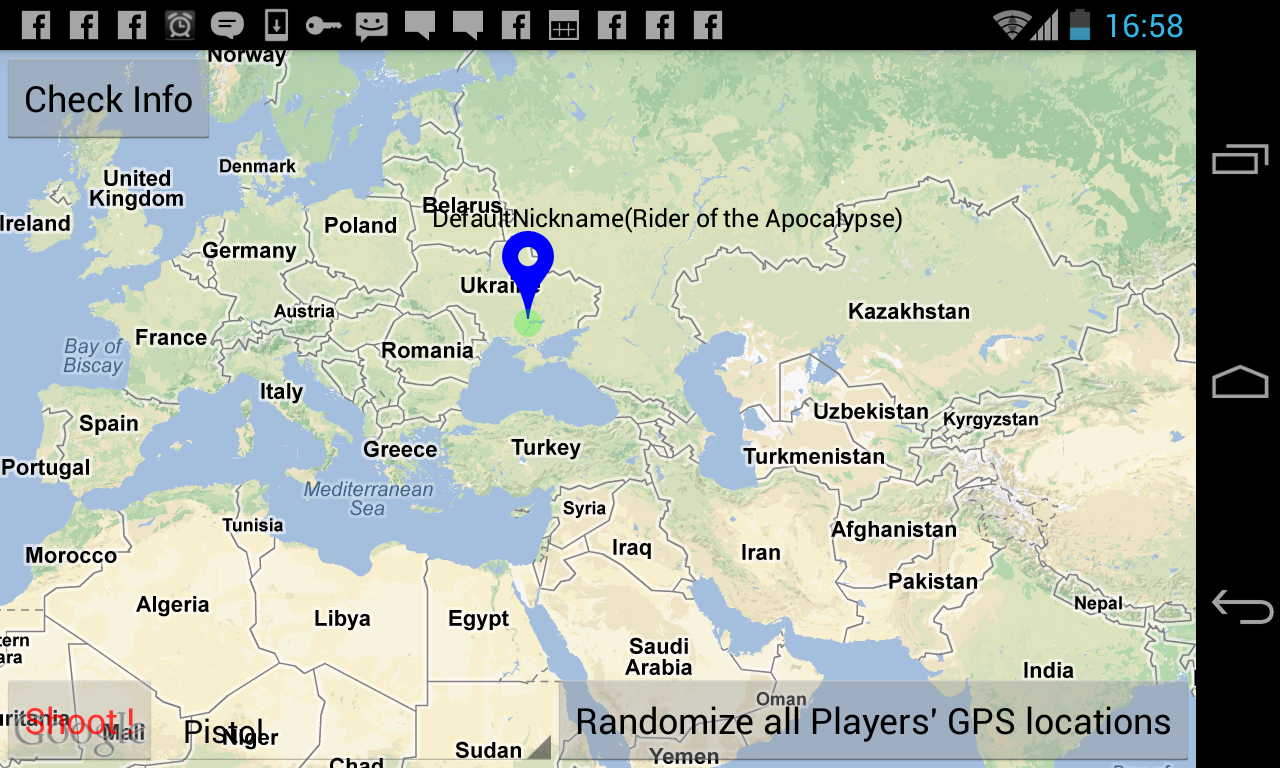
\includegraphics[height=3.5in,width=6.23in]{./images/android_screenshots/ui_prototype/UI_prototype_1.png}  
\caption{\small \sl game screen prototype \label{fig:UIPrototype1}}
\end{figure}

\begin{figure}
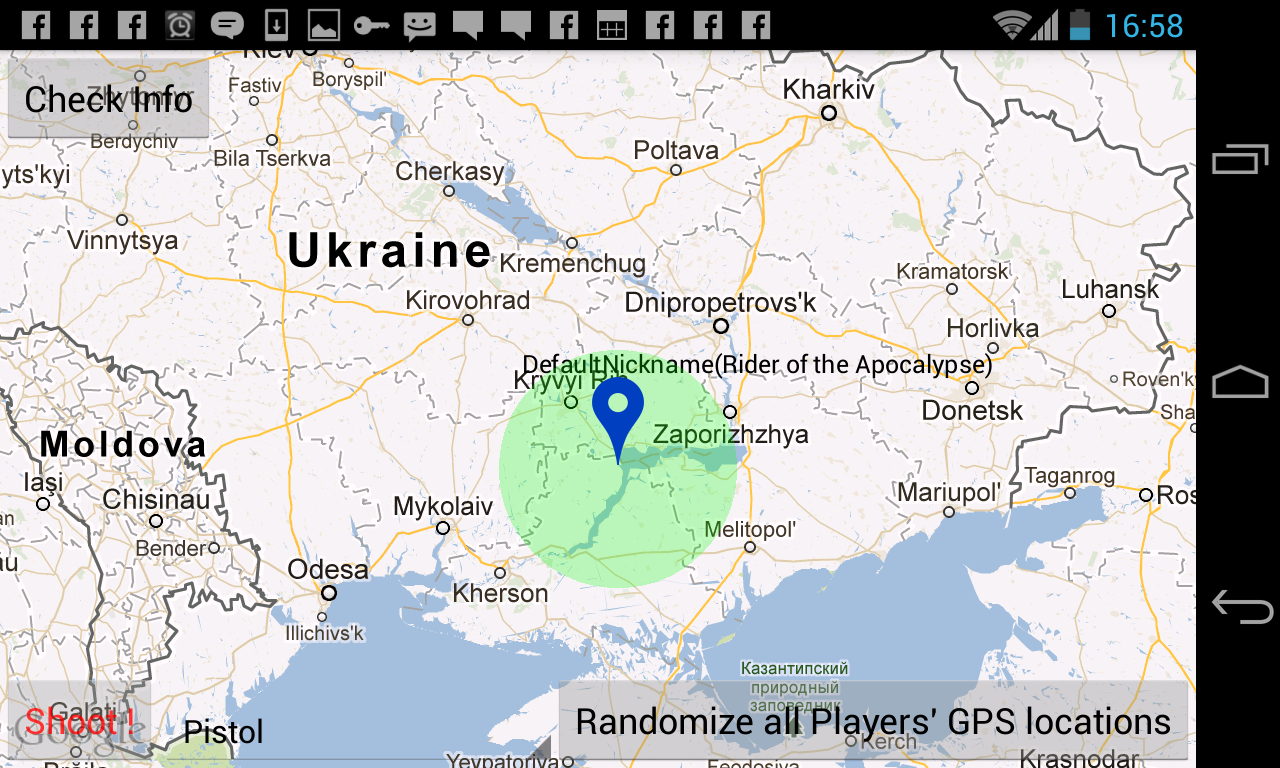
\includegraphics[height=3.5in,width=6.23in]{./images/android_screenshots/ui_prototype/UI_prototype_2.png}  
\caption{\small \sl game screen prototype \label{fig:UIPrototype2}}
\end{figure}

\begin{figure}
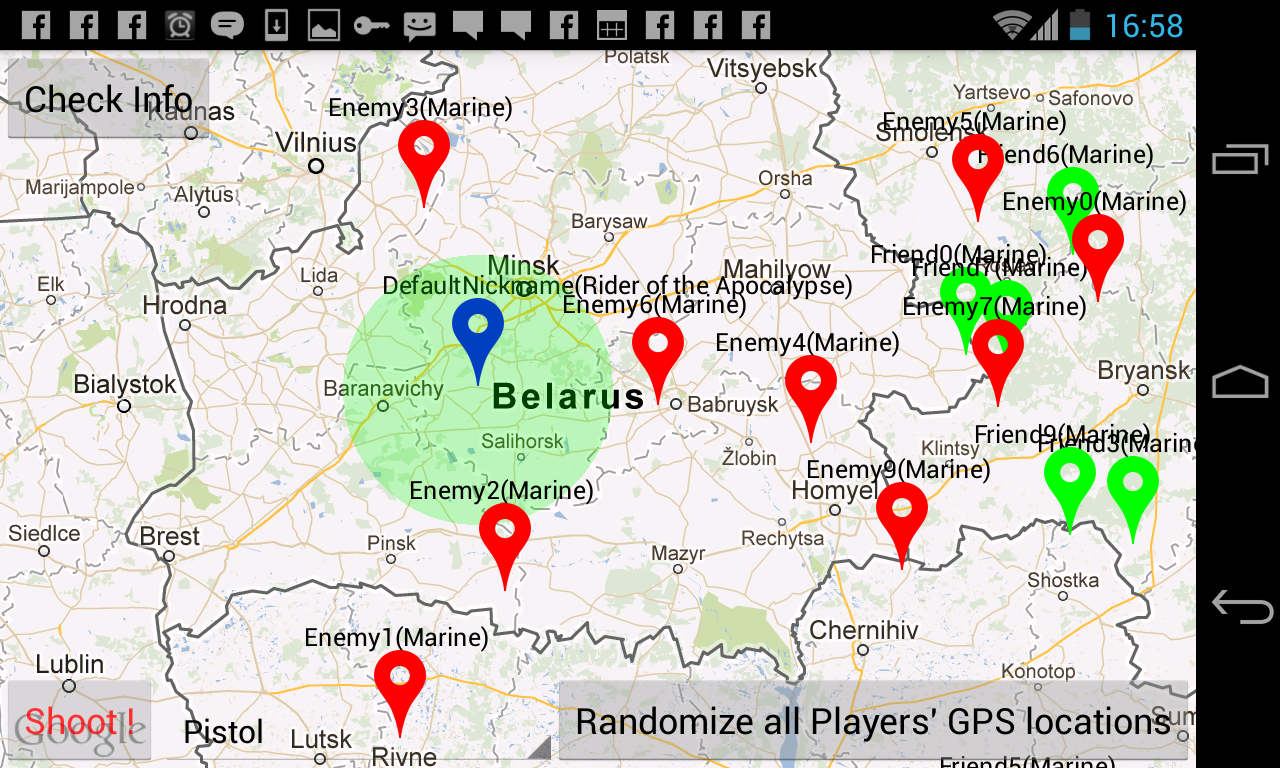
\includegraphics[height=3.5in,width=6.23in]{./images/android_screenshots/ui_prototype/UI_prototype_3.png}  
\caption{\small \sl game screen prototype \label{fig:UIPrototype3}}
\end{figure}

\begin{figure}
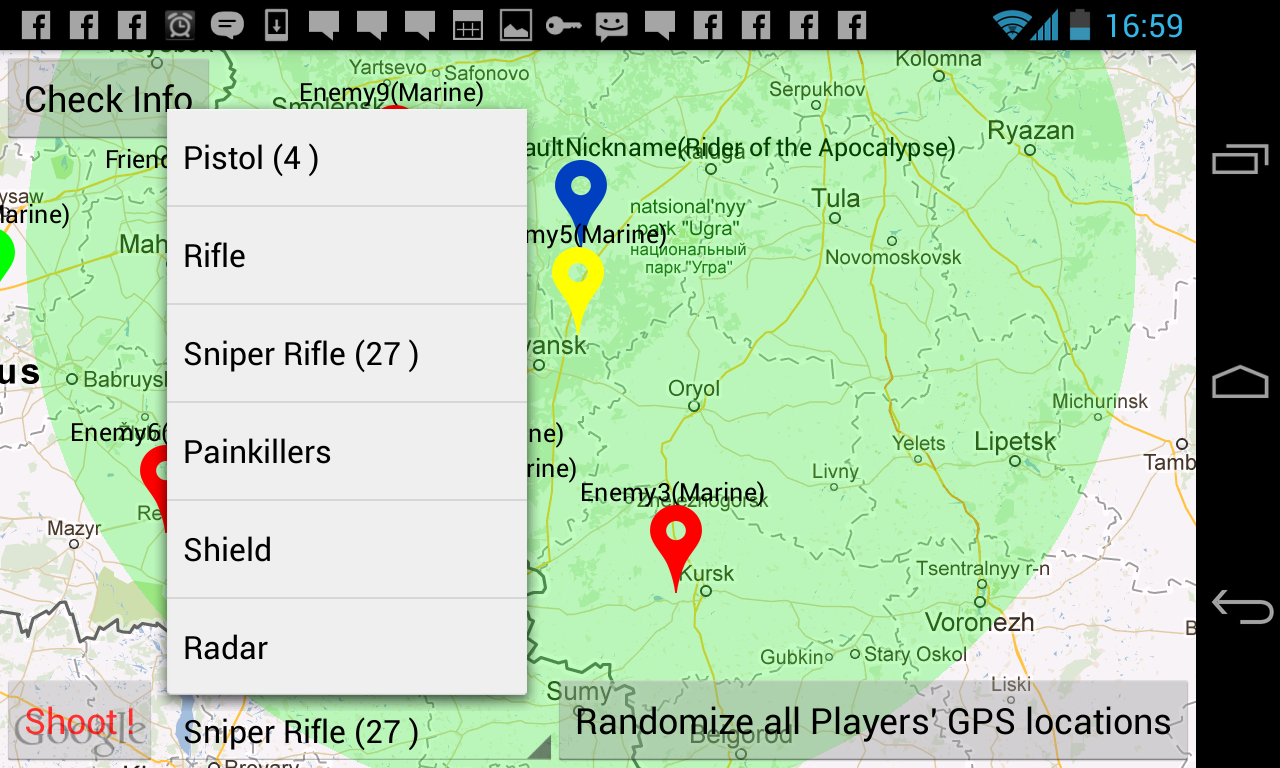
\includegraphics[height=3.5in,width=6.23in]{./images/android_screenshots/ui_prototype/UI_prototype_4.png}  
\caption{\small \sl game screen prototype \label{fig:UIPrototype4}}
\end{figure}

\begin{figure}
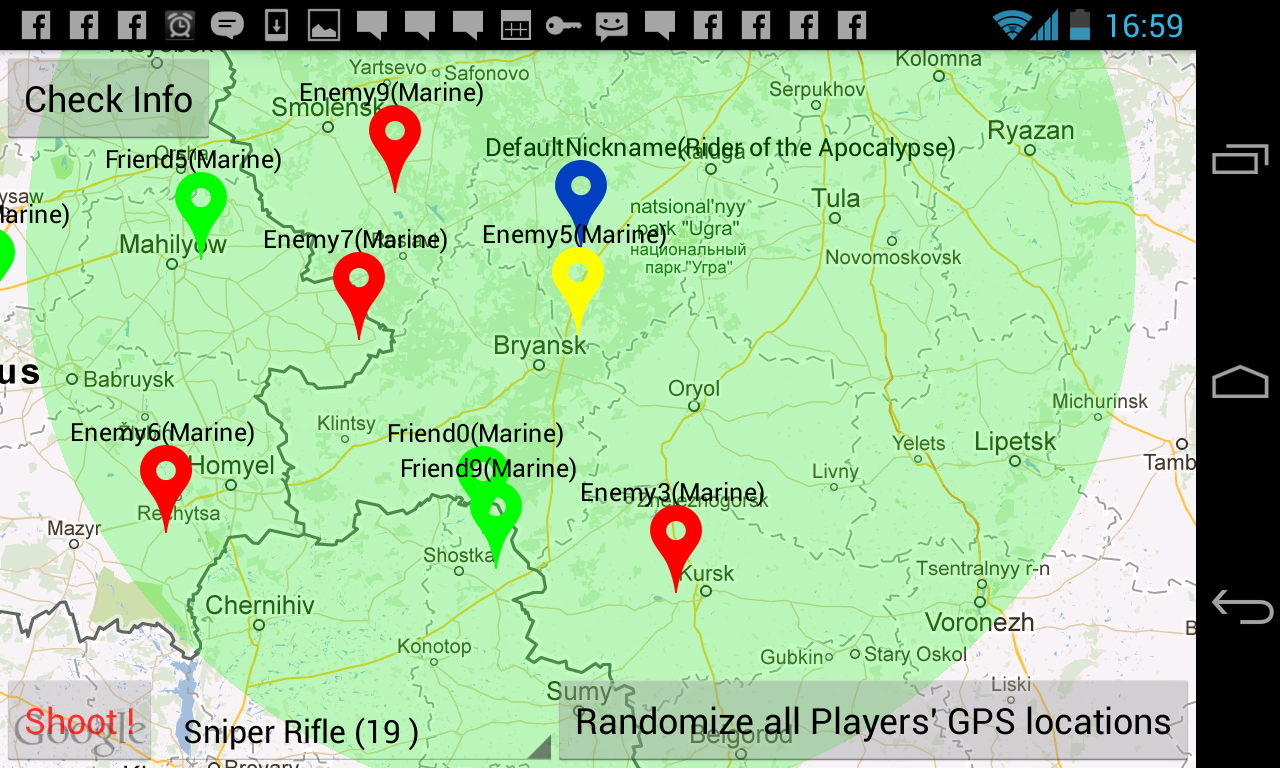
\includegraphics[height=3.5in,width=6.23in]{./images/android_screenshots/ui_prototype/UI_prototype_5.png}  
\caption{\small \sl game screen prototype \label{fig:UIPrototype5}}
\end{figure}


The creation of the game screen prototype has been followed by that of the menu
UI prototype. For starters, this one hasn't been made with easy user interaction
in mind, but rather as a set of basic functions that need to be provided
outside the game itself. Also, it has been an exercise of design. Two screens
were thought of, initially: the main menu and a lobby screen. The main menu
screen has been initially seen as only a gate to the game, an easy intro rather
than anything else. The lobby screen has been designed to functionally
accomodate what was necessary in terms of game and character preparation
- and predicted the need for another screen - that of the character settings,
marked by the presence of the button labeled 'Change my Info'. The result can be
seen in Figures \ref{fig:menuPrototype1} and \ref{fig:menuPrototype2}.

\begin{figure}
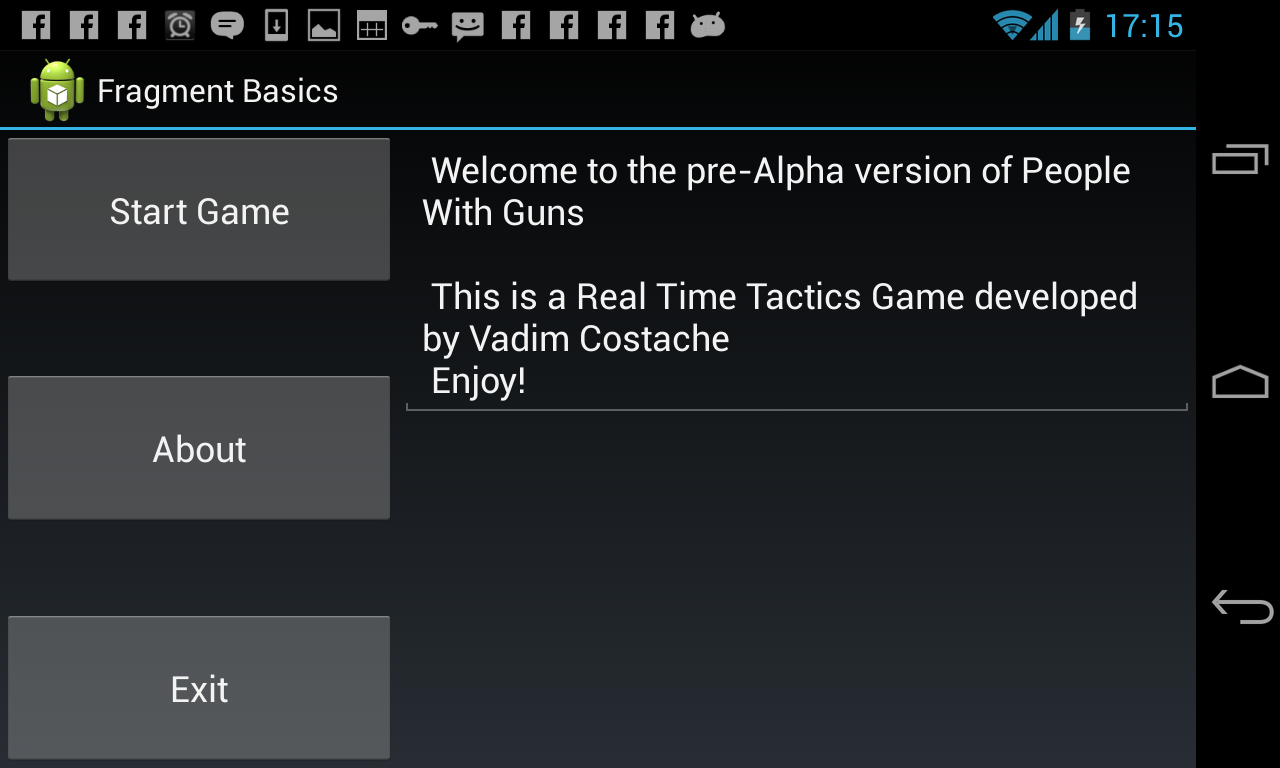
\includegraphics[height=3.5in,width=6.23in]{./images/android_screenshots/menu_prototype/MENU_prototype_1.png}  
\caption{\small \sl main menu screen prototype \label{fig:menuPrototype1}}
\end{figure}

\begin{figure}
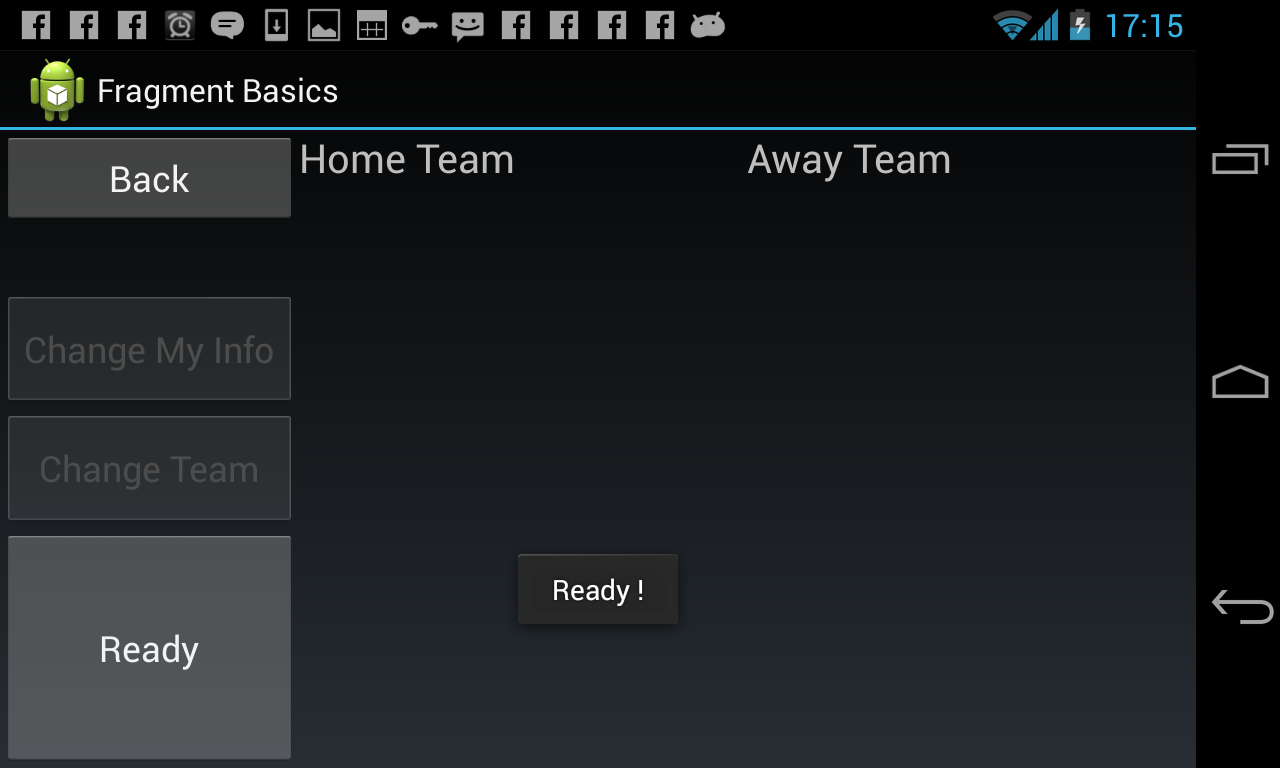
\includegraphics[height=3.5in,width=6.23in]{./images/android_screenshots/menu_prototype/MENU_prototype_2.png}  
\caption{\small \sl lobby screen prototype \label{fig:menuPrototype2}}
\end{figure}

The two prototypes have been put together in one project that has served as the
foundation of the application to come.\newline

Very soon the necessity for a settings screen right out of the main menu came up
(The server was initially run locally, on the author's laptop. The main reason
to create the settings screen was that location of the server has been changed
many times during the first stage of development - and therefore it was
necessary to re-type the IP address and port number. A button labeled 'Settings'
was added to the main menu. The settings screen came right after with just an
'OK' button and two textboxes for the IP and port inputs (as can be seen in
Figure \ref{fig:main_menu_settings}).\newline

\begin{figure}
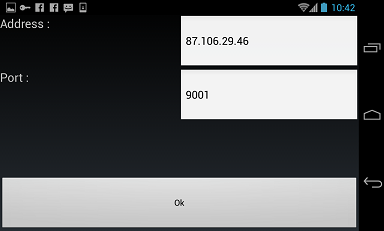
\includegraphics[height=3.5in,width=6.23in]{./images/android_screenshots/tutorial_main_settings.png}  
\caption{\small \sl The settings screen, out of the main
menu\label{fig:main_menu_settings}}
\end{figure}

At the beginning of the development, as functionality to connect to the server
has just been implemented, there was no loading screen. Instead, the application
UI would just freeze for a few thousand milliseconds. That has been considered
unacceptable from a usability perspective. The first idea was to add a loading
widget on top the main menu screen - but the separate loading screen has proven
itself a more versatile concept that can be used for functionality to come. The
loading screen had to mark the transition to entering the game. A loading screen
was added, with a simple loading widget looping infinitely and a 'Loading' text
at the bottom of the screen(Figure \ref{fig:loading}). This screen has remained
visually untouched until the last version of the application.\newline

\begin{figure}
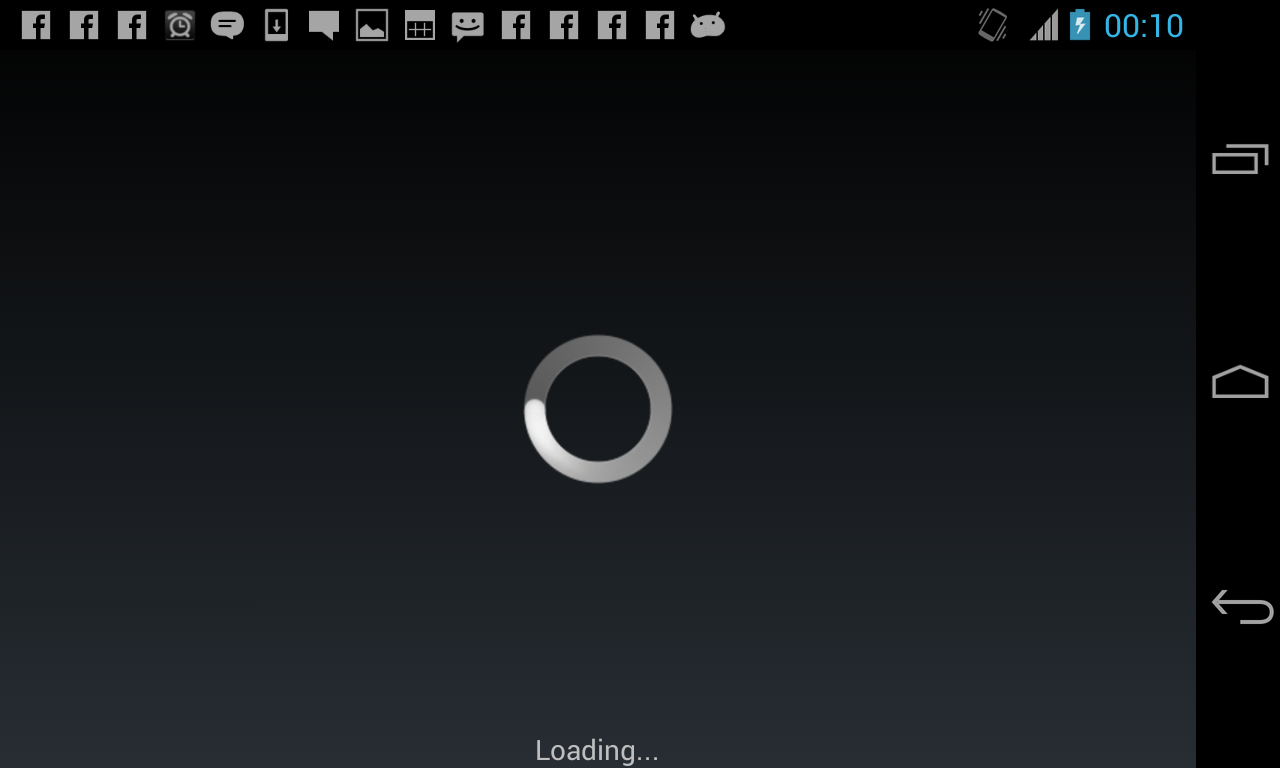
\includegraphics[height=3.5in,width=6.23in]{./images/android_screenshots/tutorial_loading.png}
\caption{\small \sl The loading screen\label{fig:loading}}
\end{figure}

Once the game client became capable of successfully connecting to the server and
setting up everything for the lobby screen, the need for the lobby settings
screen came up - and therefore the lobby settings fragment has been created -
with a spinner for choosing between characters, a textbox for the nickname, a
multiline textbox for loading the description of each character or 'profession'
and an 'OK' button. This screen has also remained largely unchanged until the
current point of development and can be observed in Figures
\ref{fig:lobby_settings_1} and \ref{fig:lobby_settings_2}.

\begin{figure}
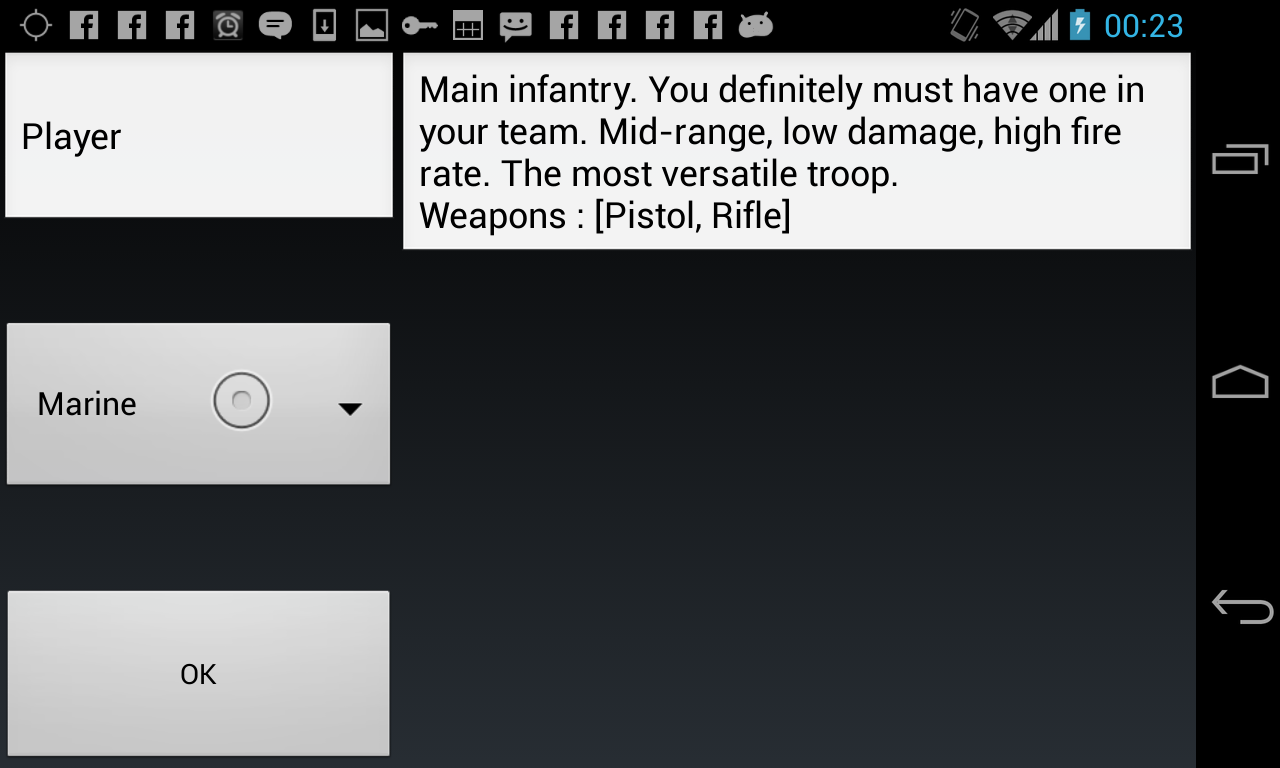
\includegraphics[height=3.5in,width=6.23in]{./images/android_screenshots/first_development/game_first_development_9.png}
\caption{\small \sl The character editing screen (a.k.a. the lobby settings
screen) menu\label{fig:lobby_settings_1}}
\end{figure}

\begin{figure}
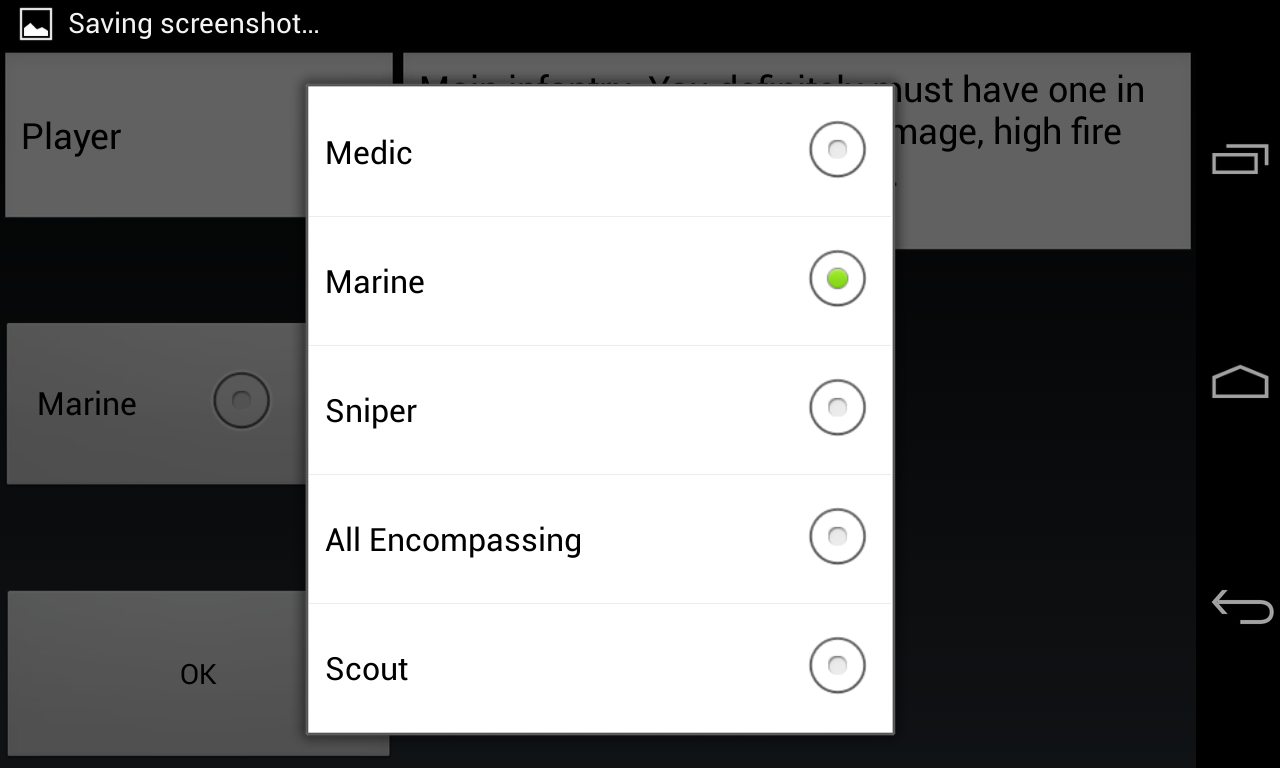
\includegraphics[height=3.5in,width=6.23in]{./images/android_screenshots/first_development/game_first_development_10.png}
\caption{\small \sl The character editing screen (a.k.a. the lobby settings
screen) with the character selection dialog opened
menu\label{fig:lobby_settings_2}}
\end{figure}


\subsection{The first testing phase}

Contrary to the original plans, the first testing phase took only half a day
with another half day of preparations. Prior live tests have been done by the
author alone, with two phones.\newline

Five people (three male and two female) were invited to play the game. Three of
them had Android phones. The other two have used the two phones that the author
had in posession at the time. Unfortunately, most of them had Android 2.2 and
2.3 installed. The preparations meant convincing them to volunteer their phones
for an OS upgrade. Android 4.0 was installed.\newline

The tests have been done mostly indoors, as they revealed various bugs in the
server and client code that were not detected when testing discrete features.
Because six people had five phones, two of them have played
alternatively.\newline

Because not all players had 3G connections available, the game has been played
by connecting to a WiFi router. The first bug we noticed was that occasionally
the game would disconnect for no apparent reason. Others have been related to
GPS devices in one of the phones not retrieving the position and crashing the
application or concurrency issues improperly treated.\newline

A few temporary quick fixes got the game working and the testers managed to play
the game, firstly indoors for a few times and then outside, while still
connected to the WiFi router. This has inadvertently been a test of the WiFi
coverage of an average old 802.11 b/g router - around 50 - 70 meters radius in
an open space describing a half-circle around the router. The author was the
first to accidentally run outside the WiFi coverage and get disconneted.\newline

After the playing was finished, the testers and the author sat down for a
focus group discussion, during which criticism of the gameplay, UI and game
satisfaction were expressed. Although the concept itself has been positively
appreciated, the game UI has received a lot of criticism. Also the random
disconnection of the game from the server has caused a lot of frustration among
the test players. A proposal has been made to allow saving the last player
status and position on the server and allow a timeout until the player would not
be allowed to reconnect. A debate led to the conclusion that enabling such a
feature could allow cheating: A player would disconnect from the game, get close
to other players, reconnect, shoot and repeat the sequence - thus avoiding
damage and causing frustration to others. \newline

Until the end of the first testing session done with a group of people, the UI
has remained largely untouched. The two unused buttons on the game screen have
been kept for tester feedback on how pleasant the position of those buttons is
for the reach of their fingers. The goal for the game UI has been to become
similar to a game controller, while having the game screen in the middle. And
the screen had to be layed out in a way in which the user would not feel cramped
when playing the game. The only addition to the UI has been the 'Settings'
button in the main menu, together with the settings screen.\newline

The first people to test the game have criticized the following aspects:
\begin{enumerate}
  \item \textbf {The game UI}: The need to reselect the target every time the
  weapon is switched has proven frustrating. The entire process of selecting
  a weapon before firing it has been regarded as too slow: the players wanted to
  be able to shoot the entire arsenal immediately, if possible.\newline
     
  The lack of control over what is happening has been criticized: The player
  health was only displayed above the head of the player, along with the name
  and 'profession'. It made it hard for players to notice changes. Notifications
  on who 'shot' who were not yet implemented. The player's health was not
  displayed anywhere. Messages could not be sent to the team. The first proposal
  has been to enable writing and sending messages, messenger style. After some
  discussions, the conclusion came that predefined messages are much more
  useful(like the ones used in the video game ''CounterStrike''), while more
  complex messages can be communicated verbally, keeping the players more
  focused on the dynamics, rather than on the technicalities of the game.
  
  \item \textbf{The menu UI}: The lobby UI has been criticized - but not for
  it's layout, but for the comprehensibility - there was no mark for the
  player's 'Ready' status, the 'Change my Info' label wasn't comprehensible. The
  nickname and 'profession' were not remembered from one game session to the
  other or from one app launch to the other. This frustrated the users - and
  they simply refused entering their nicknames after a few games. The game ended
  up with no one knowing who's who, because they had the same nickname - the
  default 'Player'. One tester complained that he wanted to click his own name
  in the team lists and get to the settings screen - but functionality
  to do that was not implemented.\newline
  
  A general complaint has been expressed towards the fact that there are no
  tutorials on how to play the game.
\end{enumerate}

The first testing phase, though short, has left a lot of guidelines on what to
do from that point on.\newline

\subsection{The second develpment phase}

The first testing phase has left a lot of 'todos', notes and guidelines for
better adapting the UI and game mechanics to the player's needs. The second
development phase has addressed these needs with a personal touch from the
author and an influence of the switch to a newer version of Maps API (V2). The
newer version of Maps API also came with the requirement that Google Play
Services be installed on each device that runs the game.

\subsubsection{The Server}

The only change done on the server in the second development phase, beyond bug
solving, has been the switch from InetAddress to InetSocketAddress as key in the
server's management HashMaps. That's because multiple connections from behind a
router with NAT were not possible. InetAddress only holds the remote IP of the
connection. The InetSocketAddress now holds both the IP address and port number
of the connection.

\subsubsection{The Client}

We will describe the changes made to the client, after the first testing phase.
The most important set of changes has occured on the UI: The Google Maps V1 API
has been discarded in favor of the V2 API, the appearance of the UI has been
radically changed and most of the back end functionality that served the game
screen has been discarded and rewritten.

The client now uses seven fragments for the UI: 'Main Menu', 'Info and
Tutorials', 'Settings', 'Lobby','Lobby Settings', 'Loading' and 'Game':

\begin{enumerate}
  \item 'Main Menu' : It has been slightly modified: The 'Start Gane' text has
  been changed into 'Connect to Server' - making its functionality more
  obvious. The logo presented in Figure \ref{fig:game_logo} has been added for
  user feedback. The 'Info and Tutorials' button has been added - it leads to
  a new Fragment that presents the idea and functionality of the game.
  
  \item 'Info and Tutorials' is a screen with a number of buttons and a
  scrollable view for displaying text and images. Here, the user will find
  instructions for the purpose how use of the app and detailed descriptions of
  the functionality of the 'Lobby' and 'Game' UIs.
  
  \item 'Settings' has not been modified.
  
  \item 'Loading' has not been modified.
  
  \item 'Lobby' : it has been slightly modified to remember the last used
  nickname and 'profession'. Each player in the team lists now shows the ready
  status of that player and a '\[ME\]' indicator has been added to the current
  player so that he can identify himself in the list. Clicking on one's own
  nickname in the list now navigates to the 'Lobby Settings' screen for
  nickname and 'profession' change. Two background images have been tried out on
  this fragment, for user feedback. They are shown in Figure
  \ref{fig:game_background_black} and Figure \ref{fig:game_background_white} 
  
  \item 'Lobby Settings' has not been modified. A background image has been
  tried out as background, for user feedback. See Figure
  \ref{fig:game_background_lobby_settings}
  
  \item 'Game' has been completely modified. Due to tester feedback and
  the change of the Maps API, it has gone through radical changes. At this
  point, the game screen looks as follows: for all the 'weapons' and 'powerups',
  buttons are aligned starting from the bottom left corner of the screen until
  close to the bottom right corner. From the bottom right corner upwards, on
  the vertical axis, three buttons and a TextView have been placed: the
  'Previous Target', friend/foe toggle, 'Next Target' buttons and a TextView
  that shows the distance from the current player to the selected friend or
  foe. If no player is selected, the presented text will be '0(Self)'.
  Otherwise, just the distance measurement is shown, with no text. In the top
  right corner, the default 'My Position' button is shown - with its specific
  icon. In the top left corner of the screen, a TextView with large text
  indicates the 'health points' of the player. Underneath the health indicator
  lays a Spinner for sending predefined messages to the team. The full
  functionality of the UI will be presented below.
  
\end{enumerate}

The typical app use scenario goes as follows: The player enters the game and
sees the 'Main Menu'. The application checks if Google Play Services are
installed and if the GPS is turned on. If either of these conditions is not met,
a dialog is presented: the player must choose to install Google Play Services and/or turn on
the GPS or exit the game. Each dialog directs the user to the appropriate Google
Play or Settings page - where the player only has to either click 'Install' or
switch the 'Enable GPS' toggle to 'ON'.\newline

Once there are no more requirements to be met in order to play the game, the
player can click on 'Connect to Server', be briefly presented with the 'Loading'
fragment and then enters the 'Lobby'. There, if the app was started for the
first time, he can see the default nickname 'Player' and the default
'profession' - Marine. If the app was previously used, the player will see the
last nickname and 'profession' used in previous runs. The server distributes the
players according to team sizes, so the player has an equal chance to see
oneself in either the 'Home' or 'Away' team. Then, the player can opt to change
the team by using the 'Change Team' button. Also, the nickname and 'profession'
can be changed by navigating to the 'Lobby Settings' screen. Once the 'Ok'
button is pressed in the 'Lobby Settings' screen, the changes are saved by the
application and sent to the server for broadcasting, and the player is returned
to the 'Lobby' screen.\newline

At the point where all the players have done setting up, they can send the
'Ready' signal. When all the players are ready (for testing purposes, one
player present on the server is enough to start a game), the five second
countdown is received from the server and the player is now facing the 'Game'
screen.\newline

In order to understand what can be done at this point, a detailed description of
the 'Game' UI is necessary: \newline

We can visualize the UI based on the screenshots presented in Figure
\ref{fig:game_ui} and Figure\ref{fig:game_ui2}. It presents the groups of UI
elements on the screen.
We shall now present all of them, separated into groups, by position
(positioning also separates functionality groups, therefore we can also state
that they are presented by related functionality). All the UI elements on the
'Game' UI are programmatically generated - and not from an XML file  :
\begin{enumerate}
  \item\textbf{The bottom of the screen, starting from the bottom-left corner}:
  The 'weapon'/'powerup' buttons are generated once the 'Game' fragment is loaded,
  based on the list of weapons specific to the player's 'profession'. They
  appear from left to right. If less or equal to three weapons are given, the
  buttons will be made slightly larger than otherwise - up to a maximum of six
  (the number of weapons featured in the test 'profession', 'All Encompassing').
  Each button press shoots the 'weapon' or 'powerup', according to a so-called
  'policy' provided in the Weapon object. The policies are as follows: 'self',
  'friends', 'friends and self', 'enemies', 'friends and enemies', 'friends and
  enemies and self'- stating on which kinds of players one given 'weapon' or
  'powerup' can be used. A button long press will draw the range of the
  'weapon'/'powerup' on the map, with the player's position in the center.
  
  \item\textbf{The bottom-right corner of the screen}: The player selection
  buttons and the distance indicator are generated on the vertical axis, starting from the
  bottom-right corner of the screen - in order, the 'previous target',
  friends/enemies toggle, 'next target' buttons, and on top a TextView showing
  the distance to the selected player or '0(Self)' if no player is selected(in
  translation, the 'self' or 'current player' is selected). The friends/enemies
  toggle is used for switching choosing between the two groups of players:
  friends or enemies. On each press on the 'next target' button,
  the next closest player from the chosen category is selected. The reverse
  applies to the 'previous target' button - which selects the previous farthest
  player if a player is selected and the closest one otherwise. The distance
  indicator serves for the use of an experienced player who knows the weapon's
  distances by heart and does not need to draw the weapon range circle on the
  map. The players may also be selected by simply tapping their respective
  markers on the map - but through testing it has been determined that in a more
  intense and dynamic situation, selection by clicking on the marker can become
  difficult and inaccurate. Both modes are supported now. At this stage of
  development, deselection of players (and implicit selection of the current
  player) is done by touching a random unoccupied area on the map.
  
  \item\textbf{The top-right corner of the screen}: The 'my position' button - 
  Clicking it will cause the map to be automatically scrolled until the position
  of the current player is centered.
  
  \item\textbf{The top-left corner of the screen}: The health indicator is a
  TextView that presents in large text the available health points of the
  current player. Underneath it lies a spinner that provides a list of messages
  that the player can send to his/her team. One can do so by clicking on the UI
  element representing the spinner, beneath the health indicator. After the
  first click, the spinner dialog appears and shows the list of messages. The
  player can send one of the messages in the list by clicking it. The dialog is
  canceled by selecting a message or clicking outside it.
  
  \item\textbf{The area in between the two top corners of the screen}: This is
  the area where the powerup duration is dynamically shown during its effect.
  This can be seen when the player casts 'invisibility' or 'shield' on oneself
  or when a friend casts 'shield' on the player.
  
  \item\textbf{The area above the weapon buttons}: This is where the
  notifications appear, in the form of Toasts. By default, a toast has a given
  lifespan - but each time a new toast needs to be displayed, it first closes
  the toast currently on display, if it is the case.  
\end{enumerate}

Although they are not yet discretized, thus far we can distinguish three types
of game that can be played with the current setup: the \textbf{Default
game}(which requires multiple players, but excludes the 'All Encompassing' game
type); \textbf{Duel}(two players choose the 'All Encompassing' profession -
receiving the entire arsenal provided by the game - and try to eliminate
each other from the game by using various strategies of combining 'weapons' and
'powerups'); \textbf{David vs. Goliath}(a small number of players choose the
'All Encompassing' profession and play against a significantly larger number of
players that use all the professions except 'All Encompassing').\newline

Until now, the default game and the duel have been tried out - and they are
fit for different situations: The default game can take up to 20 minutes and is
played on a large area (there is no limit for now), depending on the mood and
disposition for running of the players. The duel is performed usually by two
players sitting next to each other and takes two-three minutes.\newline

Thus far, no game end condition has been introduced - players who lose all
health points are notified that the game is over for them through a dialog that
gives them two options: quit the game or spectate. The second option implies
that they are marked as 'dead' on the map, cannot be selected and their weapon
buttons are removed from the screen. Still, they can watch the evolution of the
game on their mobile devices. When all players of one team are marked as 'dead'
(they have lost all their 'health points') and at least one member of the
opposing team still has more than zero health points, it can be considered a win
for the opposing team. The ending condition has not been implemented, because
for this stage of development of the application there is no reward system
implemented. \newline

The main functional differences from the first development of the game are:

\begin{enumerate}
  \item A switch from Google Maps API V1 to V2 has been done. This implied
  rewriting the whole UI and several methods in the helper libraries.
  
  \item Because of the switch mentioned above, the custom Overlay object (along
  with the custom tap and marker drawing functionalities) and the object
  responsible with position retrieval have been discarded. Position retrieval is
  done through an option provided by the GoogleMap object provided by the Google
  Maps V2 API. The whole marker and weapon range drawing are also done through
  the GoogleMap object - OverlayItem objects have been replaced by Marker
  objects and GeoPoints have been replaced by LatLng instances.
  
  \item The whole UI has been rewritten, having as a result what was described
  above.  
  
\end{enumerate}

Passive disconnection detection functionality has been added in the loop that
waits for incoming messages. The functionality of some weapons and powerups has
been modified. A powerup called `Radar` that was present in the first
development iteration, but did nothing has been removed. The 'Invisibility
cloak' and 'Knife' have been added. Powerup duration indicators have been
added.\newline

The final message structure in between the server and the client will be
presented in one of the Annexes.\newline

During the second development phase, a lot of decentralization and
modularization of functionality has been done. Some classes that only served the
Game UI relying on Maps API V1 have been removed. Others, serving the Maps API
V2 have been added. Various bugs that caused crashes have been corrected. The
starting condition has been reintegrated in the game - the weapon buttons
are disabled until a 'Start Game' signal is received from the server.\newline

\subsubsection{Logging, Testing and Data Usage}
After the first testing phase, a the need of a logging system was felt. A
logging system based on Logcat capture has been added. Uncaught exceptions are
now caught and logged before the app closes. \newline

A lot of testing has been done with the 'UI/Application Exerciser Monkey' to
show up potential bugs and crashes. Some bugs have been found and patched - but
one has persisted: Apparently, there are some humanly-impossible combinations of
keyboard and touch inputs that lead to a Spinner dialog crashing the
application. This is an Android-related issue and cannot be solved by
the author.\newline

Another bug that has persisted is that of the WiFi disconnection(3G connections
stay alive). Apparently, this is an Android bug.\newline

As for logging, a Logger class has been created, its functionality has been
extended to retrieve the data usage of the app. Because of various compatibility
reasons, the data usage of the entire device during the usage of the app is
retrieved, instead of the usage of the application itself. This means that the
data usage of, say, social network or mail applications adds to the count - but as a
general idea (and not very precise numbers) is needed, it has been considered a
decent solution.

\subsubsection{The UI}

The second development session has come with the mindset to completely change
the UI. And not only that was done: the whole underlying framework has been
changed. A switch to the Google Maps V2 API was made. A lot of functionality has
been thrown away - such as the Overlay that served for drawing the players and
for laying out the controls. A lot of new controls had to be added. A lot of
underlying technicalities have been changed(such as the custom screen tap
functionality and data objects used for positioning).\newline

Because of the switch to the new Maps API, the MapView object which served as
the container for all controls has disappeared. It has been replaced by a
GoogleMap object which is not intrinsically a View and cannot be treated thusly.
Some improvisation was required to artificially create a container for the map.
This has been done by programmatically creating a RelativeLayout and adding the
View that contained the map as a child. Then, the apparent choices have been to
either add all the controls programmatically - which is very tedious - or embed
a Fragment within another Fragment - which is bad for performance. All the
controls have been generated and added programmatically. And the result has been
previously described in the paper - having as a result the UI presented in
Figure \ref{fig:game_ui2}: The UI has been properly partitioned in four
functional areas that, although they provide much more control and
functionality, they don't cloister the map. The health of the current player is
visible, a button has been added to center the image on the current position of
the player, individual buttons are generated for the list of weapons provided
for a 'profession', a group of buttons is added for help in target selection.
Target selection by tapping on the screen has been preserved as an alternative
to the selection buttons. The latest addition - the Spinner serving message
sending was taking up too much space and hindered the view of the map. A good
solution has been to make it semi-transparent - thus, making it non-intrusive,
yet present. The ranges of the weapons are now drawn in green on demand, by long
pressing the weapon buttons. The blue circle around the player's position is the
default indication of the GPS accuracy. Thus far, it has not been removed - as
it can be useful in various gameplay situations.\newline

\begin{figure}
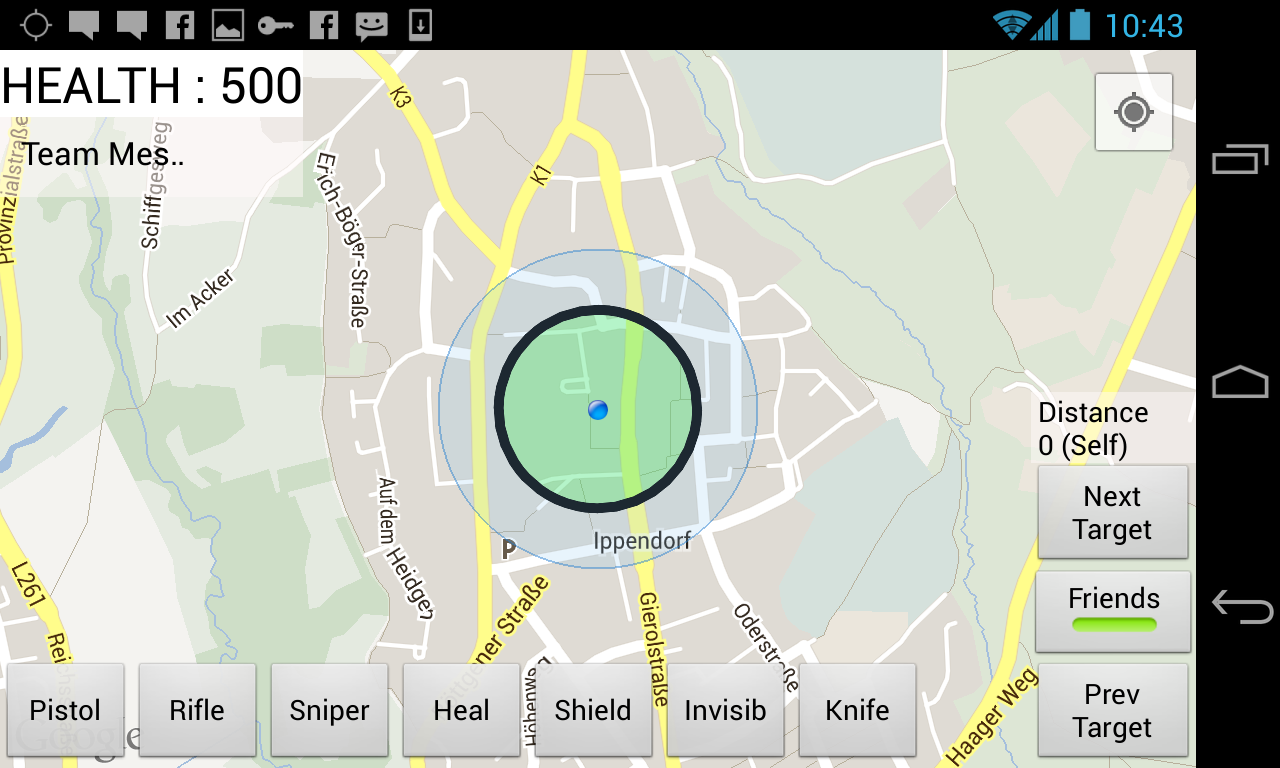
\includegraphics[height=3.5in,width=6.23in]{./images/android_screenshots/second_development/game_second_development_5.png}
\caption{\small \sl The game UI \label{fig:game_ui2}}
\end{figure}

The menu UI has also been modified:
\begin{enumerate}
  \item \textbf{The main menu screen}: The welcome message has been removed and
  place has been left for a potential logo. The addition of a logo has been
  attempted, as seen in Figure\ref{fig:logo_white}. Also, a button to navigate
  to the newly added info and tutorials screen has been added.
  
  \begin{figure}
  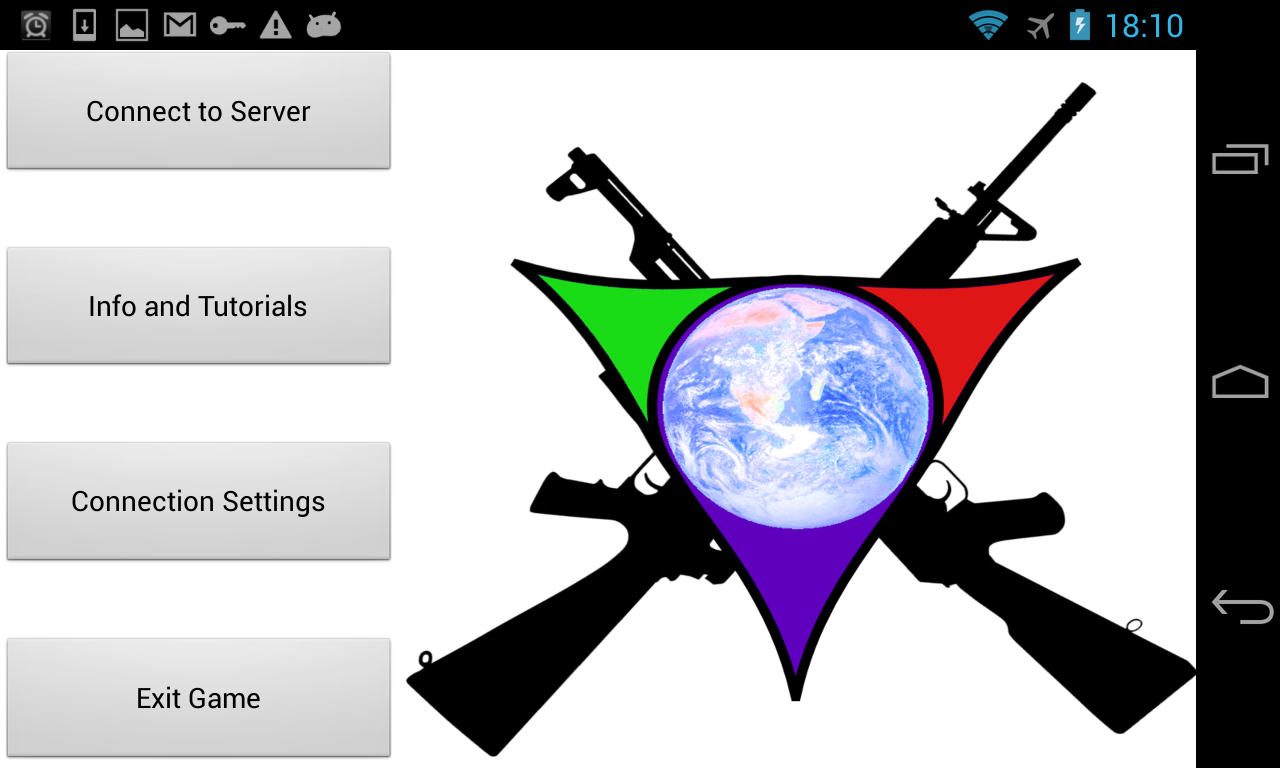
\includegraphics[height=3.5in,width=6.23in]{./images/android_screenshots/logo_white.png}
  \caption{\small \sl A white game logo \label{fig:logo_white}}
  \end{figure}
  
  \item \textbf{The info and tutorials screen}: A new screen has been added.
  It contains four buttons that lead to information and tutorials on what the
  game is and how to play it. The initial plan was to have a WebView as
  container and load the tutorial articles in HTML format. Then a simpler
  solution was devised and instead of the WebView, a ScrollView was added as
  container and a LayoutInflater object is now used to generate the
  tutoarial articles from XML files. The results can be seen in Figures
  \ref{fig:tutorial_fragment1} and \ref{fig:tutorial_fragment2}.
  
  \begin{figure}
  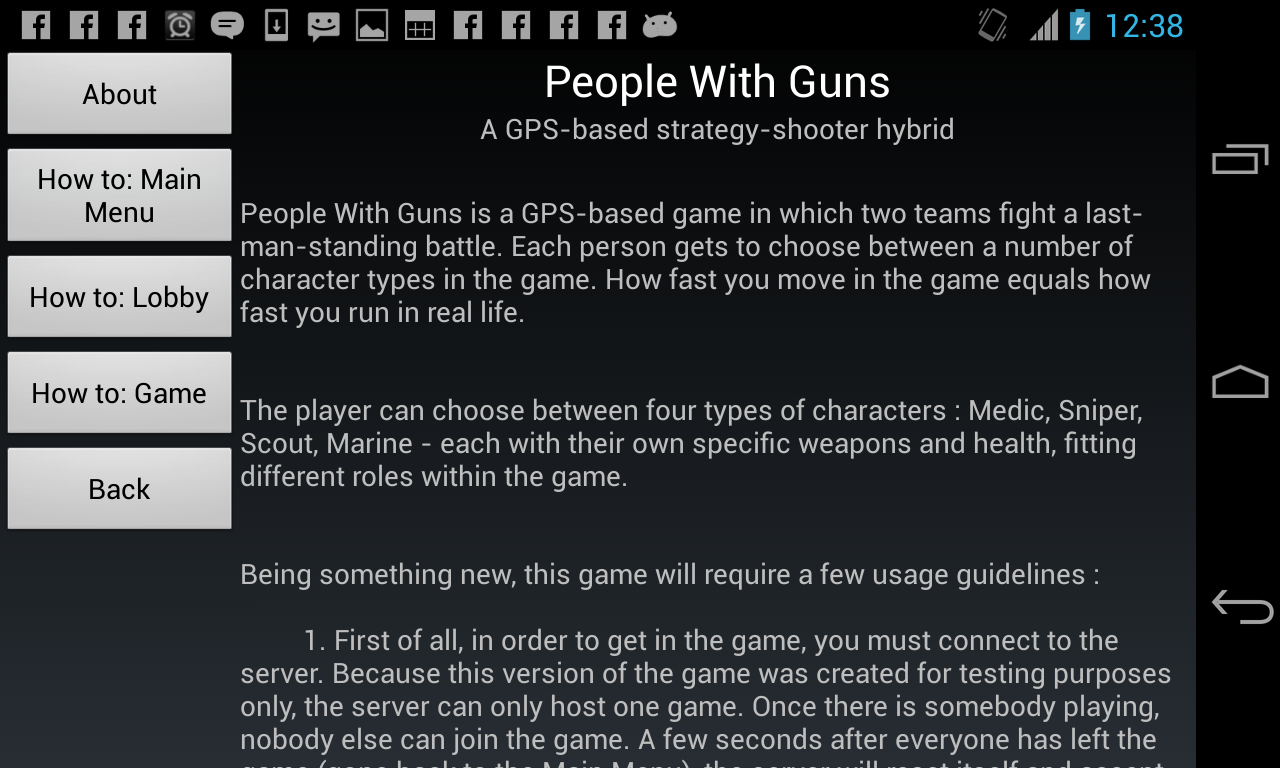
\includegraphics[height=3.5in,width=6.23in]{./images/android_screenshots/tutorial_fragment_1.png}
  \caption{\small \sl Tutorials screen: the About
  page\label{fig:tutorial_fragment1}}
  \end{figure}

  \begin{figure}
  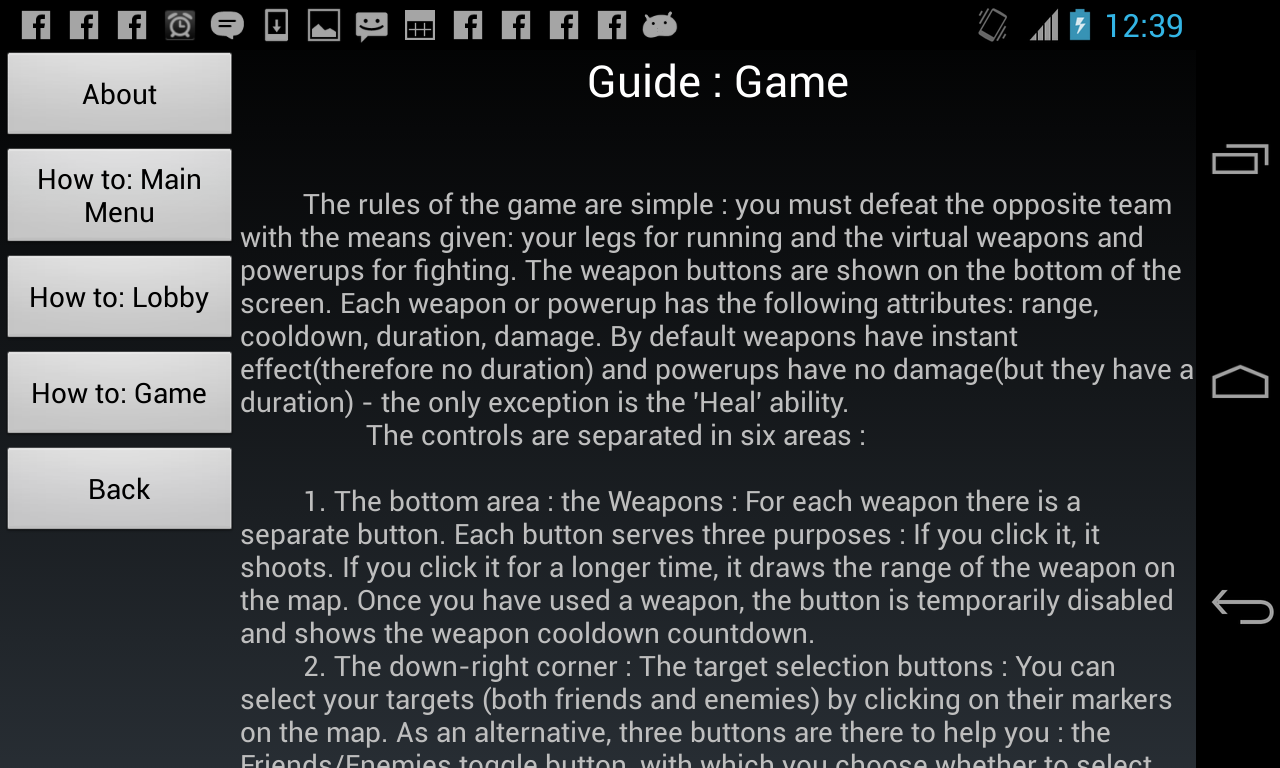
\includegraphics[height=3.5in,width=6.23in]{./images/android_screenshots/tutorial_fragment_2.png}
  \caption{\small \sl Tutorials screen: the Game Guide page
  \label{fig:tutorial_fragment2}}
  \end{figure}
  
  
  \item \textbf{The lobby screen}: The lobby screen was also modified: The
  requested feature to map the click on one's name to the character settings
  screen was implemented. Also, the ''ME'' marker has been added to distinguish
  the current player from the rest and the ''READY'' marker of one's 'Ready'
  status. Two backgrounds have been tried on this screen, as seen in Figures
  \ref{fig:lobby_background_black} and \ref{fig:lobby_background_white}.
  
  \begin{figure}
  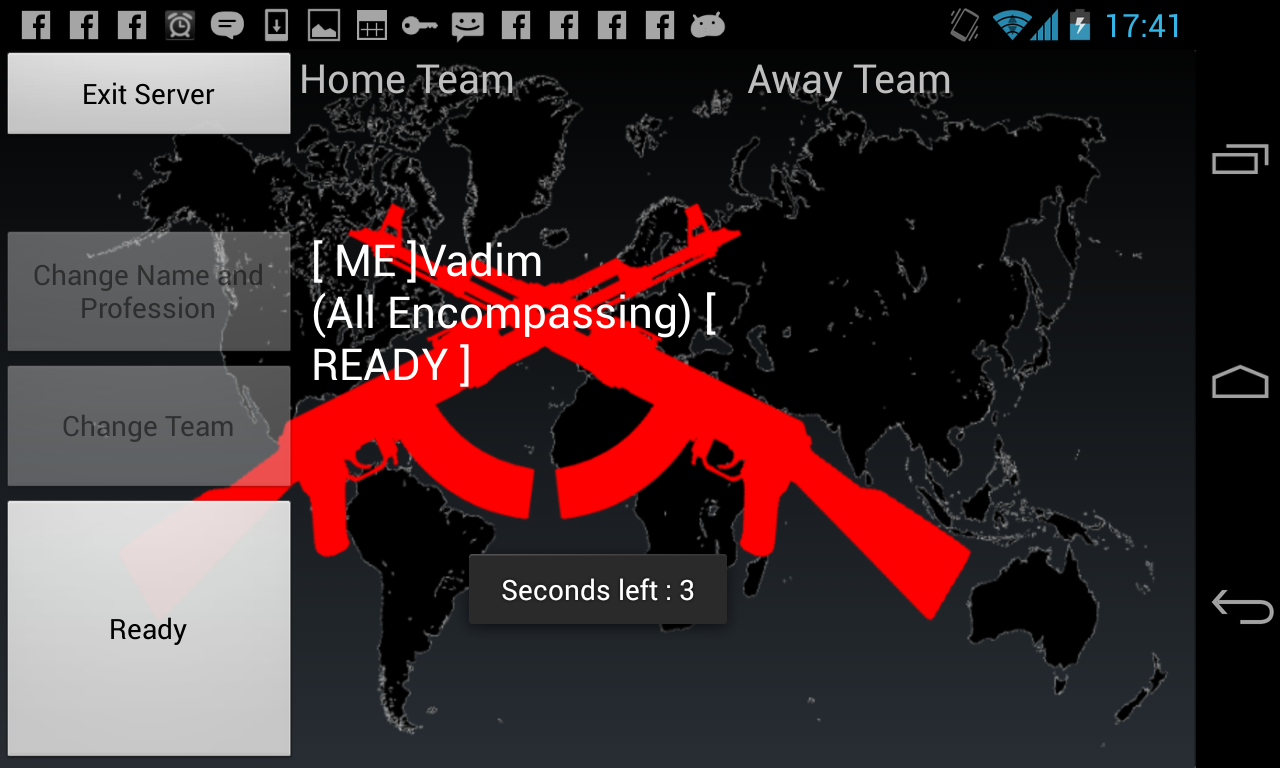
\includegraphics[height=3.5in,width=6.23in]{./images/android_screenshots/second_development/game_second_development_3.png}
  \caption{\small \sl Lobby screen with black background
  \label{fig:lobby_background_black}}
  \end{figure}

  \begin{figure}
  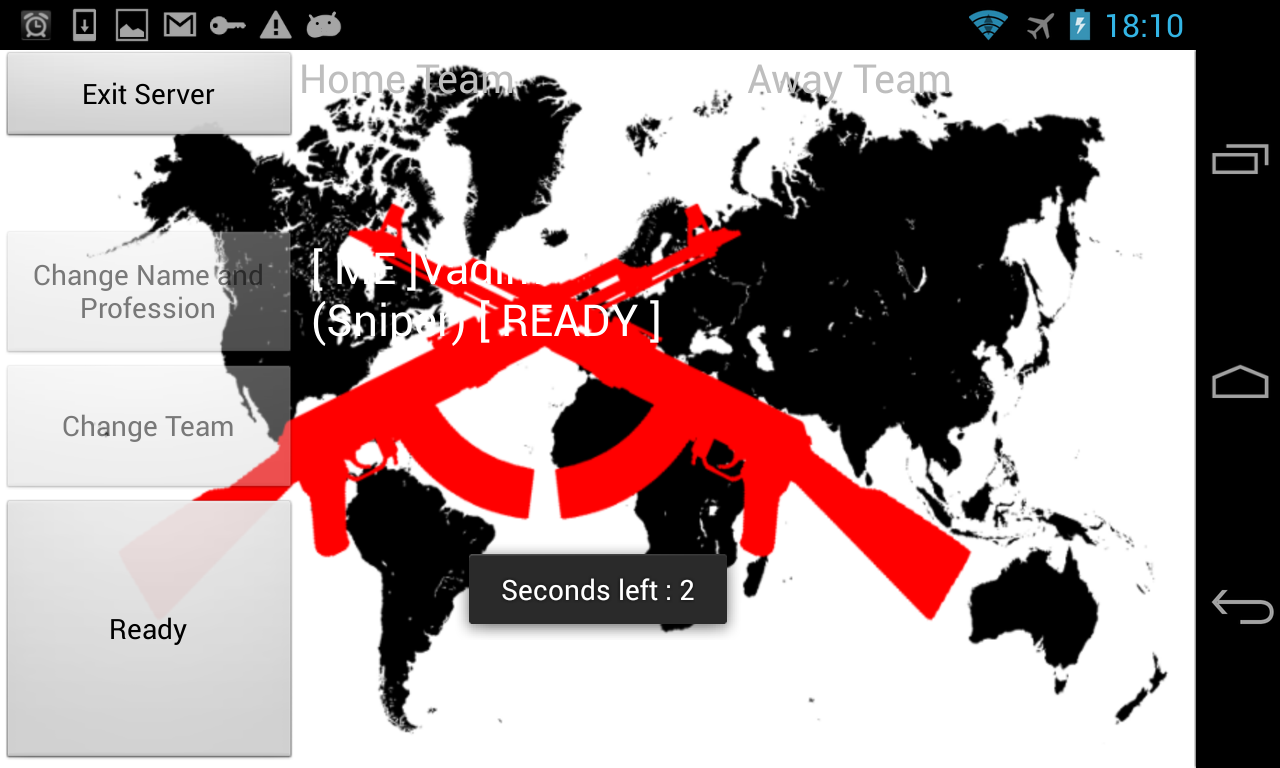
\includegraphics[height=3.5in,width=6.23in]{./images/android_screenshots/lobby_background_white.png}
  \caption{\small \sl Lobby screen with white background
  \label{fig:lobby_background_white}}
  \end{figure}  
  
  \item \textbf{The lobby settings screen}: The lobby settings screen has been
  kept almost intact since its creation. The functionality to remember the last
  used player's nickname and 'profession' was added. Also, two backgrounds in
  black and white have been tried out. They can be seen in Figures
  \ref{fig:lobby_settings_background_black} and \ref{fig:lobby_settings_background_white}.
  
  \begin{figure}
  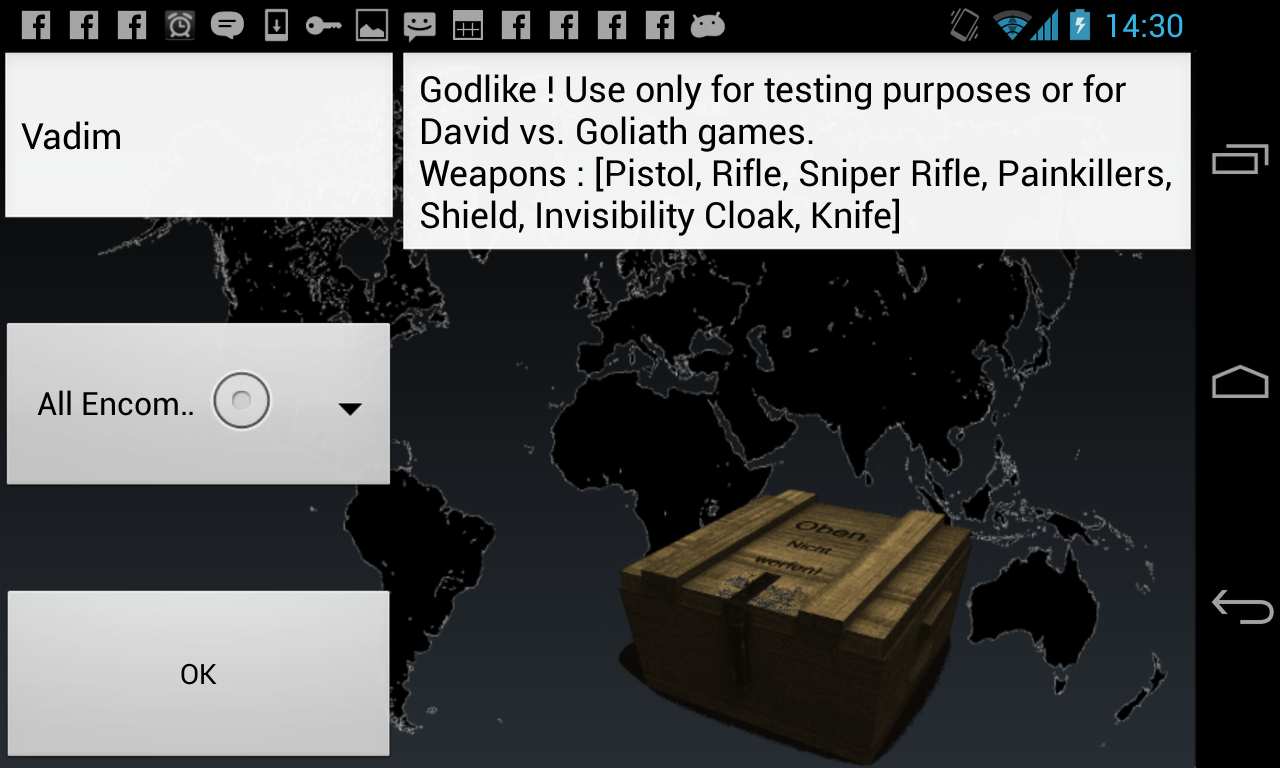
\includegraphics[height=3.5in,width=6.23in]{./images/android_screenshots/second_development/game_second_development_8.png}
  \caption{\small \sl Lobby settings screen with black background
  \label{fig:lobby_settings_background_black}}
  \end{figure}

  \begin{figure}
  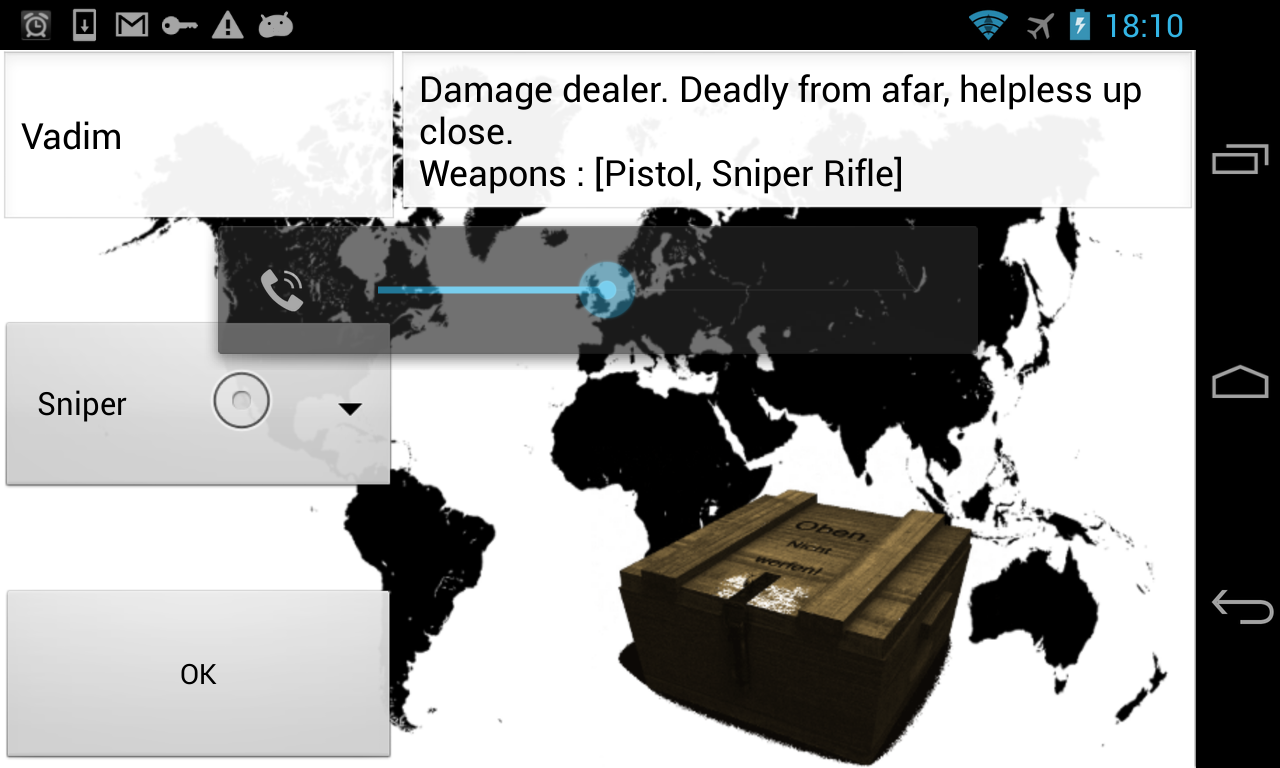
\includegraphics[height=3.5in,width=6.23in]{./images/android_screenshots/lobby_settings_background_white.png}
  \caption{\small \sl Lobby settings screen with white background
  \label{fig:lobby_settings_background_white}}
  \end{figure}
  
\end{enumerate}

\subsection{The second testing phase}

As the first testing phase, the second one has taken much less time than
initially planned - only one day. A larger number testers were invited. More
phones have been brought and almost all had 3G connections. This time, the app
supported Android versions starting with 2.3 - which made testing accessible to
all.\newline

A large part of the testing phase has consisted in the preparations: installing
the application on all devices, connecting everyone to the wireless network.
This has proven to be frustrating - therefore, everybody switched to 3G and
started to play - firstly indoors and soon after, outdoor. The UI changes have
been positively appreciated by everyone - yet a few features have proven to be
quite useless: One of them was the long click on the weapon buttons, which was
never used - because of close range gameplay, nobody attempted to draw the
weapon range. The gameplay has been very fast paced (a game lasted on average
between 10-15 minutes) and no one has actually used the functionality. The
distance indicator was not noticed at all by most testers. The health indicator,
target selection buttons and shooting functionality of the weapon buttons have
been appreciated as 'right', 'appropriate', 'useful'. A request was made for a
finishing condition and a 'You have won' screen for the winning team - and a
reward system. Because of the close-quarter gameplay, the starting condition
could not be tested - actually, a short workaround to disable it had to be
done.\newline

Unlike before the first testing phase, when few to no people interacted with
the application, before the second testing phase a large number of the friends
and acquaintances of the author have seen the application and have been giving
constant input as to whether certain aspects of the game are worthwhile or not.
Also at this point discussions on future development of the game have started. A
lot of conversations have been recorded as audio files and notes on paper. Among
the discussions, the ones on the current development have been focused on visual
aspects: The background images, the logo; a proposal to change all the markers
with 'profession'-specific ones and to replace the text on the buttons with
symbols. Besides all this, a discussion has started on the name of the
application itself. Both very positive and very negative opinions have been
expressed, but none of indifference. The first name chosen by the author for the
game has been ''People With Guns'' - but after debate and player feedback it has
been later changed to ''Gun Run''.\newline

There were ten people who actively participated in the discussions and debates
over the aforementioned aspects of the game: five male and five female.\newline

The logo has been strongly rejected by everybody - it was deemed too colourful
and unrelated to the significance of the game.\newline

The black background images used in the lobby and lobby settings screens have
been positively appreciated by the males but received mixed opinions from the
females: Three(more than half) of them said that the black backgrounds with
red weapons on top inspire violence - which should not represent the game, while
the other two have deemed them appropriate.\newline

After being presented with the white background images for the lobby and lobby
settings screens, everybody has rejected them, unanimously stating that they
break the atmosphere of the game. Everybody concluded that they prefer darker
colors in the menus.\newline

The second testing phase took a bit longer than the first. More players tried it
out, more games have been played and - most importantly - more games have been
played outside.\newline

The conclusion of the second test phase has been that the tutorials are too
long, too descriptive. The menus haven't received any criticism - but the game
UI has, in a passive manner: The long click functionality to draw the ranges of
the weapons has not been used at all. The distance indicator was not even seen
by the players and was therefore not used in any way by anyone. The
'Invisibility Cloak' powerup was used only by the current player on self, but in
the second stage of implementation it required selecting oneself(deselecting
everyone else) - this was deemed frustrating. The entire concept of selecting
oneself by deselecting all others(tapping an area on the map where no markers
are present) was deemed frustrating. Everybody playing has expressed the
necessity of symbols instead of text on the buttons and on the map. Another
aspect of criticism has been the order of the 'weapon'/'powerup' buttons: they
should be separated into two groups: 'weapons' and 'powerups'.\newline

\section{Agile planning}

The project was preceded by the search for a subject. This search has been
related to the initial plan of adding multiplayer functionality to an existing
tour app, GeoQuest. As the search lengthened, the focus diverged from the
tour app, towards GPS-enabled multiplayer games. The first ideas were for
including including small games and side activities into the tour app.
During three months, several GPS-enabled mobile games have been tried out.
Ideas from before 2007(the first iPhone) have also been scouted, along with
existing games on both Google Play and Apple's App Store. Besides that, sports
such as orienteering have been used as inspiration.\newline

The games that were found either required too much or too little involvement
from the players, required no actual movement or demanded the player to go to various
locations alone just to progress in the game. The point of this project has
become making a game that would entertain a number of people that would play
together, without the need of specific skills, know-how or prolonged
involvement. It would be played within at most 30 minutes.\newline

From all the previous ideas, the 'War Game', 'Mine Game' and 'Territory
Takeover' games were proposed. From all three, the 'War Game' was chosen for
development, while the other two have been kept for future work. On the 14th of
January, at the end of the three month exploration phase, the work has
started.\newline

In the proposal for the project, the 6 month time has been separated in four
parts :

\begin{enumerate}
  \item \textbf{First phase of development - 2 months}: During the first
  iteration of development, the most basic features of the game were to be
  implemented: basic server functionality that would allow the game to work,
  basic client functionality and the 'War Game' with the most basic features.
   
  \item \textbf{First phase of testing - 1 month}: During this phase, the game
  and its functionality would be live-tested for feasibility and quality. New
  ideas would be sought and documented. Most importantly, player feedback would
  be gathered. 
  
  \item \textbf{Second phase of development - 2 months}: During the second
  iteration of development, the 'War Game' would be completed and, using its
  framework, the 'Territory Takeover' game would be implemented. Bugs would be
  removed and tweaks would be made to the framework and the game concepts to
  match the player feedback.
  
  \item \textbf{Second phase of testing - 1 month}: During the second evaluation
  phase, both games would be tested for playability, player feedback would be
  gathered and the written paper would be completed.
\end{enumerate}

This schedule has proven unfeasible - not because of the length of the
development phases, but because of the very short length of the testing phases.
It has also been concluded that implementing two game concepts would only
greatly reduce the depth of research and would most likely provide incomplete
user experiences. The 'Territory Takeover' game has been left as future
work. Another big part of the development of this app has been played by the
continuous search for the appropriate technologies and practices for the project
- including organizing:

\begin{enumerate}
  \item The exploration phase - Creating a UI test (Android), a server test
  (in NodeJS, then Python, then Java), a client test(Android). There have also
  been some short UI tests and discussions along the way. This phase took around
  two-three weeks.
  
  \item The initial development phase - Creating a functional app with the Maps
  API V1 and writing a full-blown server. This was the longest phase - taking
  around one month and a half. No compatibility libraries were used, and
  therefore the app required Android versions of 3.0 or higher.
  
  \item The first testing phase - It lasted for half a day. Preparations for it
  took another few hours (upgrading the OS on two phones from Android 2.3 to
  4.0). A few friends of the author volunteered their Android devices.
  The application has been installed on all their phones and tried out for one
  hour (in multiple attempts, with some crashes). After playing the game, a
  focus group - style discussion was set up, the subjects being the usability,
  mechanics and feeling in and out of the game. Notes were taken, while
  everybody was discussing various aspects of the app. Also the menus and a
  possible logo were discussed. Even though the time has been short, enough
  input was gathered to change the appearance and workings of the application
  almost completely. Also this is when the decision has been taken to make the
  app compatible with Android 2.3 for the least (almost 50\% of Android users
  had this version on their phones at the time).
  
  \item The second development phase - Another three weeks were required to
  completely construct a new UI according to the requirements from the testing
  phase and the switch from Google Maps API V1 to V2. Crash logging and data
  usage logging have been added to the app.
  
  \item The second testing phase lasted one day. This time, the number of the
  people who participated has doubled - ten people. Most of them also had 3G sim
  cards. The game was finally field tested. Another focus group - style
  discussion has been set up and the opinions and suggestions were noted down.
  
  \item The documentation phase is ongoing. This is the paper documenting the
  development of the app.
  
\end{enumerate}

\subsection{Kanban}

For managing the development steps of the app, a simplified Kanban board was
mainly used. As is specific to Kanban, stories have been gradually proposed and
fragmented them tasks, where necessary. As the work for this project has been
solo, all team aspects of this organizational system have been removed. The
fields that have been kept are an 'Input Queue' of three slots, two
'Development' slots, two 'Integration' slots and three 'Live slots'.\newline

This board has been custom made for this project, unlike the typical Kanban
board - a whiteboard with slots defined by lines drawn with a marker, on which
the stories and tasks were held with magnets. The custom approach to make the
board, even though more time consuming, has proven more efficient for the
long term of the development of this application. When a whiteboard is used,
stories and tasks and magnets are lost - losing stories is something this
project cannot afford. The markers get misplaced and paper is often not found.
For the development of the app, the Kanban board was made out of an actual
wooden board, on which transparent plastic envelopes of two different sizes were
placed as slots for the stories and tasks. Also, under the board, three more
slots have been added : one for the papers for the stories and tasks, one for
the utensils(markers and pens of various colors and scissors) and the last one
for the finished stories and tasks that did were pushed outside the board. This
gave better control over the location of everything needed and multiple stories
could be placed in the same slot. For example, the two 'Input Queue' slots have
proved to be not enough for the influx of ideas and proposals for modification.
Also, the 'Live' slots were not used for single stories, but for groups, as will
be described below. The Kanban board can be seen in Figure \ref{fig:kanbanBoard}.Its
extension is presented in Figure \ref{fig:kanbanBoardExtension}.\newline

\begin{figure}
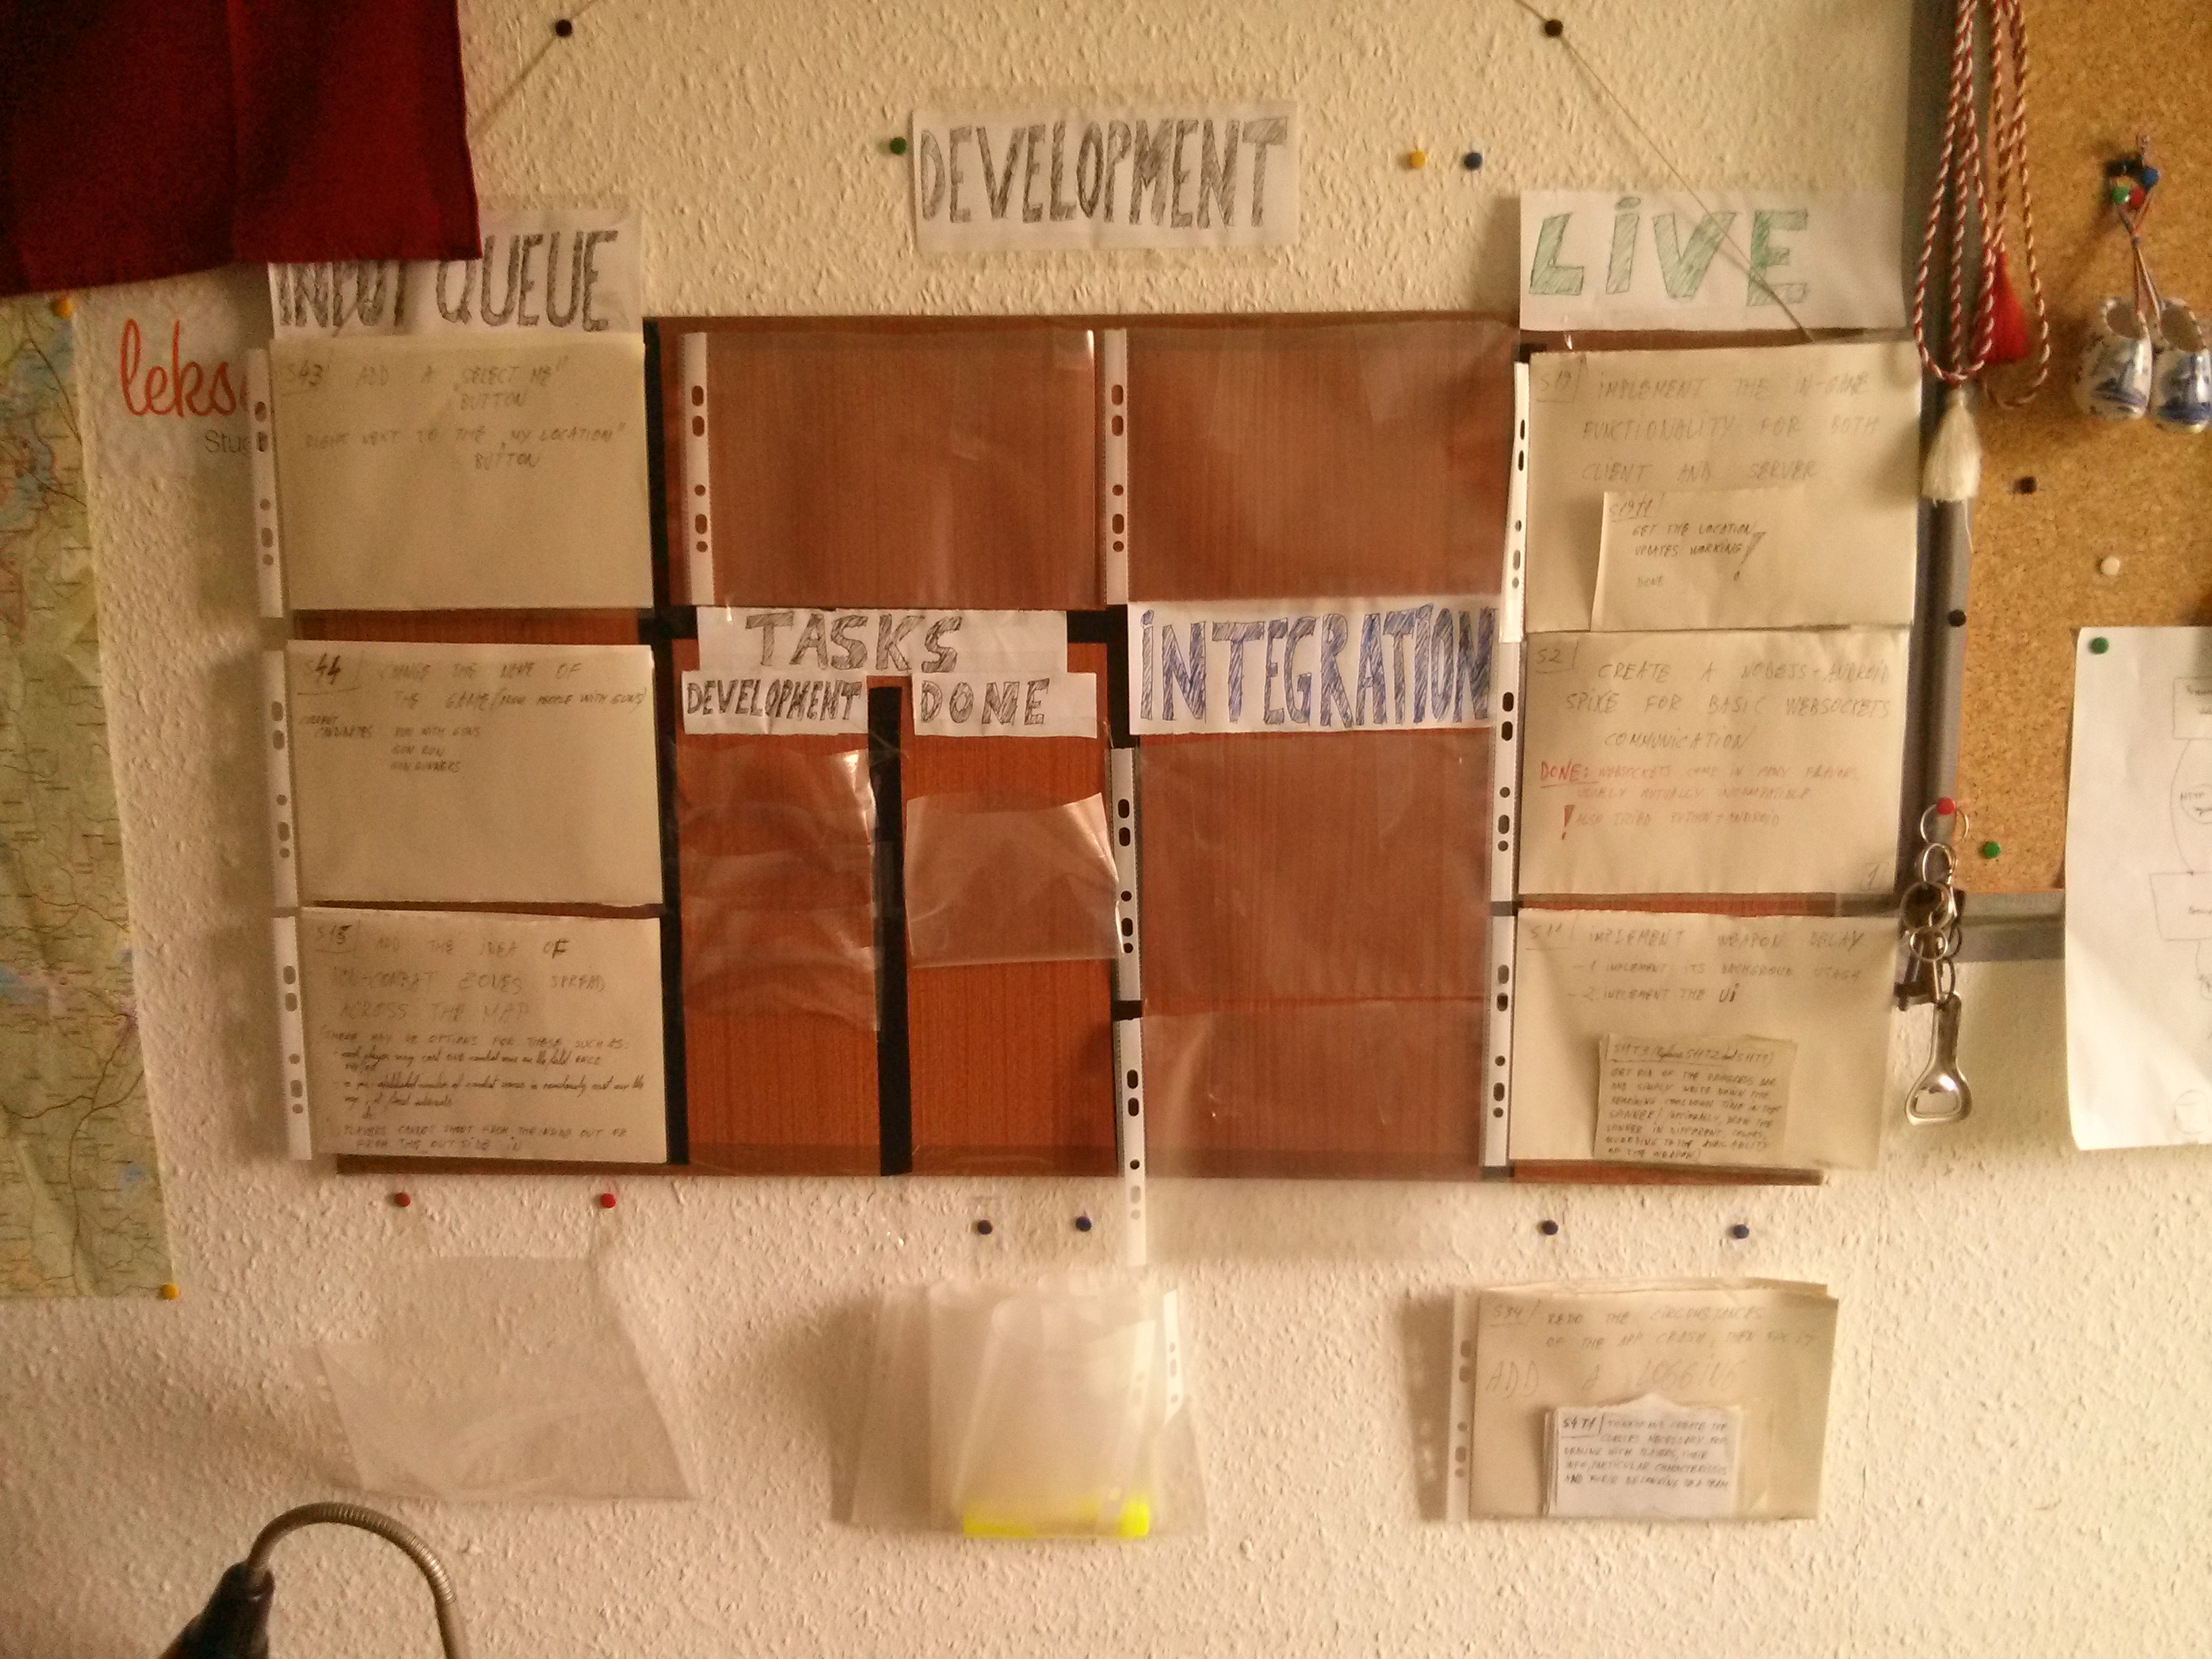
\includegraphics[height=3.5in,width=6.23in]{./images/kanban/kanban_board.jpg}  
\caption{\small \sl Kanban board \label{fig:kanbanBoard}}
\end{figure}

\begin{figure}
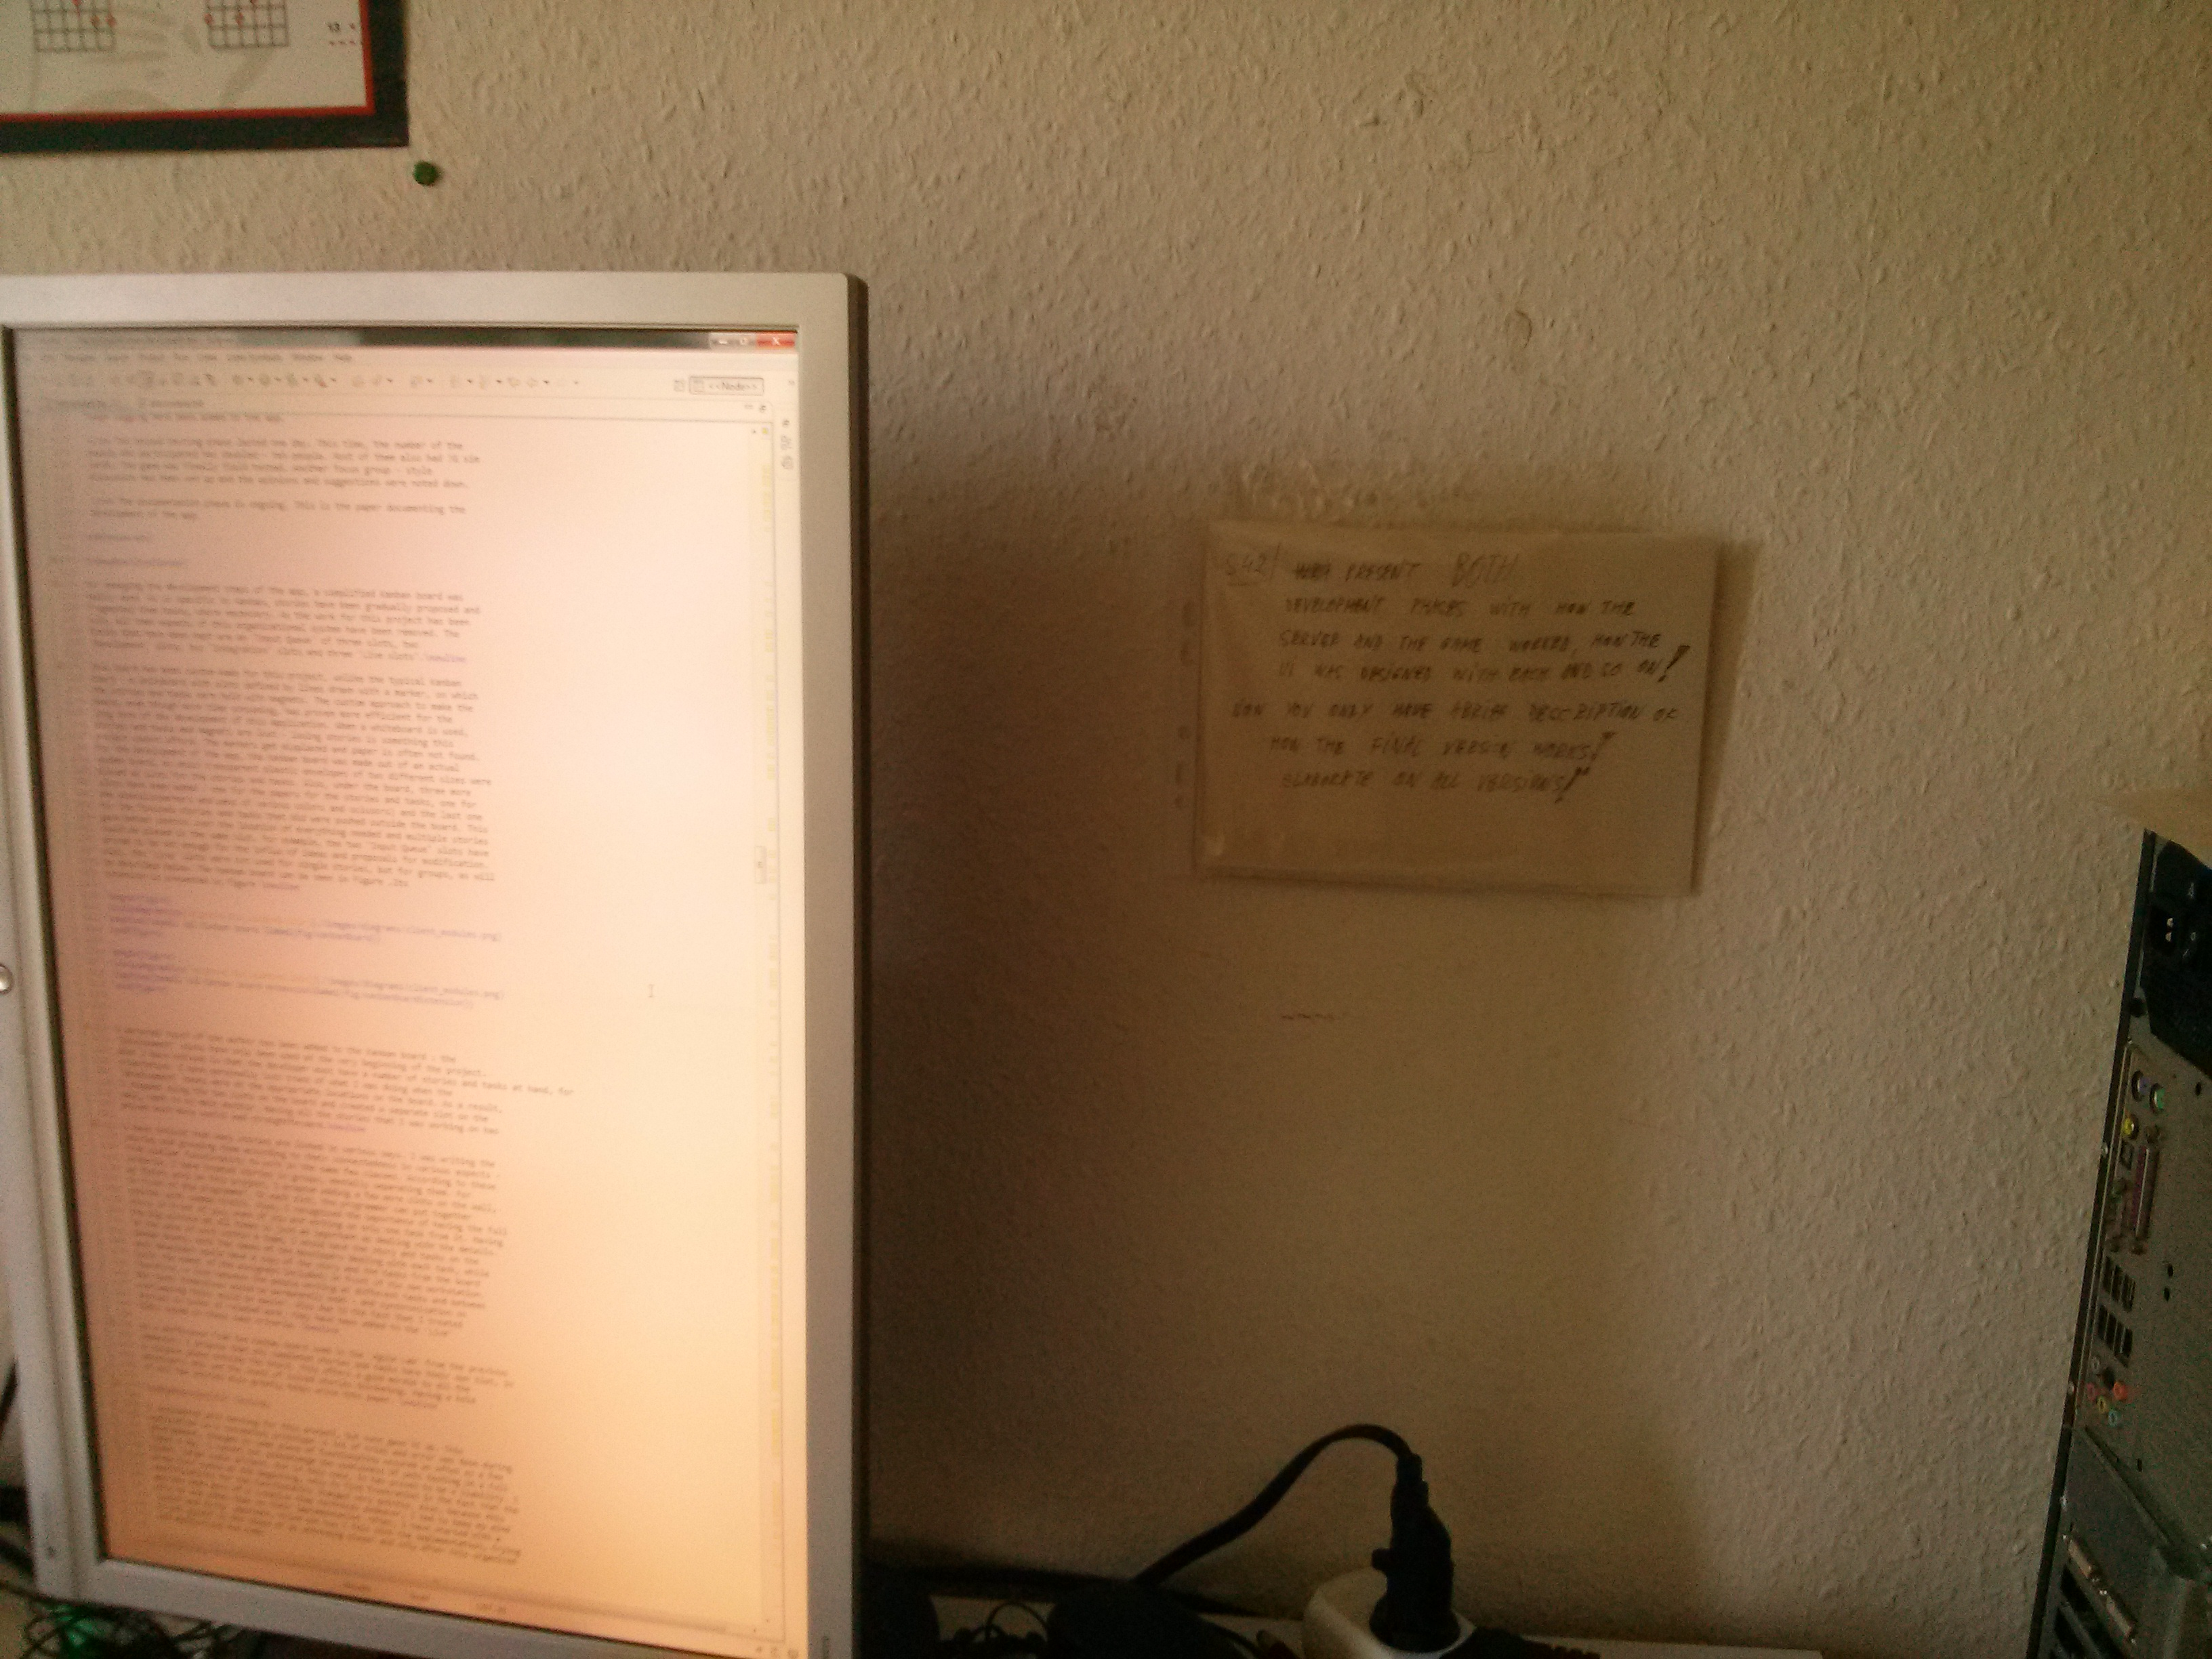
\includegraphics[height=3.5in,width=6.23in]{./images/kanban/kanban_board_extension.jpg}  
\caption{\small \sl Kanban board extension\label{fig:kanbanBoardExtension}}
\end{figure}


The Kanban board has been modified in one further aspect: As the 'Development'
slots have only been used at the very beginning of the project, they have been
brought closer to the programmer. The developer must have a number of stories
and tasks at hand, for orientation - it is easy to lose track of what must be
done, when delving into the unknown. As a result, the two slots on the board
have ceased to be used and a separate slot on the wall, next to the development
machine has been created. Having all the stories at hand has proven much more
useful and straightforward.\newline

Another observation is that many stories are linked in various ways.
During this project, stories have been grouped according to their connectedness
in various aspects - from similar functionality to work in the same few classes.
According to these criteria, stories have been treated in groups. For future
work on this project, we propose adding a few more slots on the wall, in front
of the programmer. In each slot, the programmer can put together stories with
common traits. Also, the importance of having the full story in front of the
developer has been noticed - even if one is working on only one task from it.
Having the big picture at all times is just as important as dealing with the
details. Therefore, for the case of work within a team, we bring the following
proposal: have the story and tasks on the Kanban board, with the names of the
developers dealing with each task, while each developer would have a copy of the
story and the tasks from the board (with the names of the assignees included) in
front of his own workstation. Therefore, a link between the people working at
different tasks and between the tasks themselves would be permanently kept - and
synchronization on overlapping tasks would be easier. Also due to the fact that
stories have been treated in bulks of related work, they have been added to the
'Live' slots based on these same criteria. \newline

Besides all, having all completed stories and tasks have their own slot, in
a visible place outside the board, has proven beneficial. It provides good
morale to the developer who sees the stack of solved stories thickening.
Having a hold of all the stories also greatly helped write this paper. \newline

\subsection{Unit Testing}

Unit testing has been considered for this project, but was soon given up. This
application is a conceptual prototype. A lot of trial and error was done during
development, changes to some pieces of functionality occurred as often as a few
times a day. It is hard not to acknowledge the usefulness of unit testing in a
full blown, large scale project. But in this case, it has proven to be a
liability. At the beginning, writing unit tests has been attempted, only to be
abandoned in frustration -  the specifications for the functionality changed
very quickly. A lot of refactoring and hand testing each new piece of
functionality has kept the application mostly bug-free throughout the
development.

\subsection{Choosing the technologies}

The original plan was to develop and Android and iOS app, using a development
framework such as PhoneGap. This would assume Javascript / JQuery programming
for the UI and application back-end. The communication was planned to be
established through Websockets. Therefore, for optimum performance, NodeJS was
to be used on the server side. For the location presentation, the Google Maps
API was to be used. 

\subsubsection{Unified vs. Native Frameworks}

Once an idea of how the game should look like was crystalized, a search was
made for unified frameworks for cross-platform mobile development. The first
choice was PhoneGap, which has been previously used by the author. The other
frameworks considered have been Titanium SDK, Sencha and Corona. The
multi-platform APIs offer the benefit of the 'code once, deploy everywhere'
philosophy, at the cost of performance \cite{nativevscrossplatform}
\cite{nativevscrossplatform2} \cite{nativevscrossplatform3}.
In this case, the approach of using a platform-agnostic framework is
disadvantageous. The discussion on which one is better can be resumed to the
conclusion that none of them is appropriate for the development of such a
game.\newline

And here are the reasons : 
\begin{enumerate}
  \item The game is fast-paced and will require a fast back-end as well as a
  front-end that is as fast as possible. The cross-platform frameworks
  essentially interface only some of the native functionality and display the
  app through a webview - requiring Javascript or a Javascript-based framework
  for creating the interfaces. These frameworks have been previously tested by
  the author. The outcome has been disappointing. Qooxdoo, ExtJs and JQuery were
  tried out. Qooxdoo performs faster than the other two, but makes it very slow
  and tedious to develop a complex UI and almost impossible to add extra
  functionality. Still, it is slow for the purpose and feels nonnative. After
  reading a few articles that compare Phonegap, Titanium, Sencha and Corona, it
  has been concluded that with or without various advantages and disadvantages
  between them, they are all similar in performance - and therefore too slow for
  the development of this game.
  
  \item Developing native code can prove to be easier, as the Android
  development community is much larger than that of Phonegap developers, for
  example. The support is both more intensive and extensive for native
  platforms. 
  
\end{enumerate}

From this point on, the unified frameworks have been given up and a decision had
to be made between iOS and Android development. Android was chosen.


\subsubsection{Communication Protocols}

A list of protocols have been proposed before beginning of this project: 

\begin{enumerate}
	\item WebRTC - A protocol that is to be part of the HTML 5 standard. It will be
	based on the RTP(Reliable Transport Protocol), which is the base for VoIP
	protocols and is itself based on UDP. It promises to be a very fast standard
	protocol, appropriate for audio and video streaming and massive multiplayer
	games.\cite{webrtc} It is still in draft format and there are no official
	implementations for it. Implementing the protocol itself is outside the scope
	of this project.
	\item WebSockets - A protocol that is part of the HTML 5 standard. It is a low
	latency TCP-based protocol that promises to replace Http in several types of
	web applications.\cite{websockets}
	\item TCP - One of the most intensely used two Internet transport protocols in
	digital communication today. It is designed for transmission reliability.\cite{tcp}
	\item UDP - The other one of the most intensely used two Internet
	transport-level protocols in digital communication today.\cite{udp}
	\item RTP - The protocol on which VoIP and WebRTC are based. It is based on UDP
	and it is designed for real-time streaming of data.\cite{rtp}
\end{enumerate}

Further on, when the design of the application was in progress, all unreliable
protocols have been discarded. TCP and Websockets were left in the discussion.
Initially, the use Websockets for the client-server communication was planned.
The reasoning behind it has two main arguments : 
\begin{enumerate}
  \item Websockets is an HTML5 protocol currently presented in draft by the
  IETF. This protocol provides reliable two-way communication between a server
  and a client and manages various complex issues or network features that come
  above TCP. This future standard is developed to replace HTTP and add
  functionality for technical aspects that HTTP was not covering. The reason for
  using Websockets for the client-server communication was that it promises to
  abstract a lot of protocol management issues, while offering speeds close to
  plain TCP. Also, for the game to run properly, UDP and its child protocols
  cannot be used - total reliability is required in the communication. 
  
  \item Websockets communication can be implemented in NodeJS, which is a
  framework well suited for fast-paced message exchanges and which has been
  proven more scalable than, for example, Apache Tomcat.
\end{enumerate}

As was decided to develop the server in NodeJS, the first choice was to use the
Socket.IO Websocket plugin. For the client side, Autobahn for Android was
chosen. The alternatives for Autobahn at that time were not free. After
developing a basic Websockets client with Autobahn for Android, communication
between the two was attempted. It did not work. After a search it was found out
that the protocol draft version that Socket.IO is using is different than that
used in Autobahn, and unlike Autobahn, Socket.IO uses an HTTP handshake for
establishing the connection. The Websocket-Node and ws NodeJS libraries for
Websocket communication were tried out afterwards. Neither were compatible with
Autobahn for Android. Then, Autobahn for Python was tried shortly and an
attempt to use Autobahn for Android in a Java project has failed. It was then
decided to give up Websockets and start off with pure TCP. Because writing code
in two different languages might be slower, the server has been written in Java.

\subsubsection{Google Maps API V1}

The first version of the app used Google Maps API V1. It has been chosen
because it had the most community support and the author had absolutely no
experience with Android development and the Google Maps API.  Unfortunately, the
Google Maps API and the Android Support Library cannot work together at the same
time, because they need to subclass different Fragment classes. Therefore, this
enforced the initial development to be done without the support library and
therefore the application has initially supported only Android versions equal or
higher than 3.0.

\subsubsection{Map Overlays}

The Google Maps V1 API supports the use of Overlay objects to draw on top
of the map. Most tutorials found online make use of the so-called
ItemizedOverlay, which enables easy integration of multiple location markers.
Using this Overlay subclass was attempted, but given up. Here are the
conclusions: \newline
\begin{enumerate}
  \item The ItemizedOverlay uses features that we may call 'magic'. The
  ItemizedOverlay object uses an ArrayList for storing the map markers as
  OverlayItem objects. It also needs a function that gives it the size of the
  ArrayList and redraws them automatically. This was bad on both the
  organizational aspect of the development and that of performance. Not all
  markers have to be redrawn at the same time.
  
  \item The fact that the markers are redrawn automatically has proven difficult
  to work with. For starters, there is no control over the draw process. Then,
  the OverlayItem objects cannot be stored in another data structure, such as a
  HashMap - which is used in keeping track of the players in the game.
  
  \item Because of its design, the ItemizedOverlay is fast, but useless for the
  purpose of this app. It was chosen to replace it with a custom Overlay.   
\end{enumerate}

As a replacement for the ItemizedOverlay, work on how to create a custom Overlay
that would fit the needs of the application was started. This has also permitted
the dynamic change of the marker icons, according to the needs of the game
mechanics and UI. Functionality was added for this particular feature. \newline

A real challenge was to add proper onTap() functionality for the custom Overlay.
The advantage of the already-given-up ItemizedOverlay was that it handled
position marker touch events. The new, custom overlay had no such thing
implemented. What was done was to get the pixel resolution of the screen, along
with pixel density data from the system and consider a 0.2 inch radius around
the center of the touch on the screen (this is what has been estimated to be
a circle to describe the tip of an average human adult finger). That 0.2 inch
radius in pixels has been translated in a radius, in meters, on the Google Map.
All markers inside that radius were considered and the closest to the center of
the touch was chosen. This made choosing a marker out of both crowded and loose
situations relatively easy and natural. The tutorial for this will be added as
an annex to the paper.\newline

\subsubsection{Google Maps API V2}

The use of the Google Maps API V1 ended when the absolute need to make the
application compatible with Android version 2.3, the most widespread version -
encompassing almost 50\% of the devices in use at the point of change. The
compatibility libraries require the use of a custom FragmentActivity and custom
Fragment, FragmentManager, FragmentTransaction objects. The Google Maps V1 API
requires a MapActivity to work. This comes into conflict with the
FragmentActivity. In a fortunate turn of events, the change has been done when a
total revamp of the game UI was also required.

\subsubsection{Google Maps API V1 vs. V2}

The migration to V2 is very destructive and at first feels quite unnatural. The
entire logic is changed. In V1, the map is rendered through a MapView object
that can be manipulated in a more direct and intuitive manner - lower level
access is both possible and needed. In contrast, the V2 map is accessed through
a GoogleMap object, which is no longer subclassing View. Therefore, it cannot be
manipulated in the same manner. Adding markers is done through the .addMarker()
method of the GoogleMap object. The same applies to drawing circles. Now lists
must be kept for all drawn objects, not for future redrawing, but for being able
to remove or change them. The entire Fragment object, along with a lot of
helper classes had to be rewritten completely. All methods helping out the
onTouch event for the custom Overlay were not necessary anymore. Also many
refresh workarounds were thrown away and in the process.


\subsubsection{Android development}

It must also be mentioned that learning how to program in Android was done while
developing. This was often a trial-and-error process, covered with the
author's personal takes on the tutorials found mostly on forums and blogs.



\section{Future work}


This project has served as a proof of concept, a demonstration of the
potential GPS-based Real Time Tactics games. It has proven to be enjoyable
and easy to play for everybody who tried it.\newline

During the development and testing of this application, requests and ideas have
come up for future versions of the game. They will be presented in
order:\newline
\begin{enumerate}
  \item Icons will replace the names of all weapons and the professions of the
  players. A logo will be added and the menus will have suitable backgrounds.
  The current backgrounds are to be replaced.
  
  \item A further step in the development of the game would be to add RPG
  elements to it: The game mechanics will be modified to add elements of
  realism. Weapons will receive an optimum range attribute: Shotguns will be
  most effective in close range, rifles at longer range. Damage will be
  calculated based on range versus optimum range. 'Missing' a shot will become a
  factor in the game. Skills to use some weapons more effectively or to receive
  less damage will be subject of improvement. Health will also be subject of
  improvement. Two play modes will be added: casual and professional. In
  professional mode, players will be able to take the game to a further level
  and become competitive. They will be able to improve the damage dealt with
  weapons, if they used them a lot. The accuracy with certain types of weapons
  will be subject of improvement. In casual mode, all characters will be on the
  same level - thus allowing people to play, regardless of their daily
  implication in the game.
  
  \item Another aspect to the game will be adding an incentive for travel and
  discovery. Each player will be able to get temporary or permanent items by
  exploring the surroundings of his neighborhood or travelling to remote
  destinations.   
  
  \item An MMO game will be developed, having this game and its variants as
  subgames. The concept is as follows: An application will be linked to a social
  network, such as Facebook. Players will be able to log into the application
  with their Facebook accounts. They will set up who can see them on the map and
  who they want to see themselves: only themselves, friends, friends of friends,
  etc. They will be able to interact with each other directly through the app
  and invite each other to play games, such as the one developed here. Details
  such as creating custom avatars will be provided through the application or
  through a website. A scoring system will be added and competitions will be
  held through the app - they will be advertised through Facebook events.
  Joining the event will ensure participation in the competition. Facebook
  statuses might be published by the app, if the player wants so: entering,
  winning or losing a game, retrieving items, various accomplishments can be
  subject of publishing as Facebook status updates.
  
  \item Quests will be ultimately added to various locations, if it is deemed
  reasonable. This is still subject to debate, as the quests will likely be
  location-dependent and the game experience will then vary greatly from
  country to country or even from city to city.
  
\end{enumerate}

Other various technical modifications will be made to the game: In the first
improvement iteration, Websockets will be implemented as communication protocol.
Also, creating a server that would host a larger number of games is a priority
(now the server can only host one game).






\section{Conclusion}

The purpose of this project has been one of exploring a gap within the
conceptual construct of location-based mobile games, that of location-based Real
Time Strategy games. Because no other implementation exists at the moment this
thesis is written, this has been an exploration into the unknown, a search for a
viable combination of gameplay elements that would bring enjoyment to the
players and help kick-start the concept.\newline

The exploration of ideas was carried throughout all genres of location-based
games(from Adventure to Massively Multiplayer Online(MMO) games) and a bit
further, among sports that predate the mobile phone itself. It has been noticed
that, like video games(PC and console), most location-based games focus more on
the story and immersion, than on social interaction and physical exercise.
Although there is a significant number of location-based multiplayer games,
their gameplay experience is largely solo and sedentary, with social interaction
narrowed down to a limited number of in-game actions.\newline

''People With Guns'' has addressed these aspects of gameplay, by exploring
Milgram's reality-virtuality continuum starting from a set target for the
reality aspect - a game that would entice players to move and communicate
directly - and adding virtuality in a suitable amount that would add to the game
experience.\newline

As the field testing has proven, the goal has been achieved: All the game
testers have enjoyed it: a roughly fifty percent female - fifty percent male
population, ranging from the age of 18 up to 27 have enjoyed playing and
requested the opportunity to play again. This has set a foundation from
which further development, testing and exploration can be done.\newline

The application developed during this project has proven to be a socially
engaging mobile game with the potential to be adopted by a broad spectrum of
population, with or without technical skills or gaming background. As half of
the population of game testers has been of non-gamers and they found it easy to
get started and enjoy the game, we can safely say that ''People With Guns'' has
been a success on this thread of exploration, too. \newline

With ''People With Guns'' - now called ''Gun Run'' - a new niche has been
created in the genre of location-based games. That is of location-based Real Time
Strategy games.\newline







\begin{appendices}


\section{Game and game platform websites}



\nocite{teamtags}
\nocite{gps1}



\textbf{ARIS Games}: http://arisgames.org/\newline

ARIS Games is a framework for developing Adventure/Investigation games. Most
applications of these games have been within the education area.\newline

\textbf{Tourality} - http://www.tourality.com/\newline

Tourality is a mobile application that allows people to play a number of racing
games. Among them are single lap or multiple lap races, capture the flag races
where players have to run towards a given marker on the map. The first one to
reach the marker gets one point - and another marker is randomly generated
elsewhere. This last race game has represented an important source of
inspiration in the construction of the idea for the game developed on this
project.\newline

\textbf{Wherigo} - http://www.wherigo.com/\newline

Just like ARIS, Wherigo is a toolset for creating Adventure/Investigation
games.
\newline

\textbf{conTAGion} - http://www.2clams.com/\newline

Contagion is a GPS-based zombie apocalypse Massively Multiplayer Online game in
which the players are either in the role of zombies or humans, evading or
attacking each other. The game can also be played in single player mode. A game
has been attempted, but due to a difficult and buggy interface, it was
not considered worthwhile.\newline

\textbf{Shadow Cities} - http://www.shadowcities.com/\newline
 
Shadow cities is an MMMORPG(Massively Multiplayer Online Role Playing Game) in
which the player is put in the role of a mage. The mechanics of the game tend to
be similar to those of classical MMORPGs, but they now involve the map and the
GPS. The player has to travel around physically in order to reach various areas
where levelling may be done.\newline

\textbf{SCVNGR} - http://www.scvngr.com/\newline

SCVNGR is a social game that uses Google Places for checking in, creating or
accepting various challenges already left by others at given places.\newline

\textbf{Please Stay Calm} - http://pleasestaycalm.com/ \newline

Please Stay Calm is a single player GPS-based zombie apocalypse RPG game in
which the player has to scavenge or fight zombies in various areas from the
map.\newline


\textbf{Parallel Mafia} - http://www.parallelmafia.com/ \newline

Parallel Mafia is a GPS-based MMORPG in which the player builds up his own
mafia, cooperates with or fights others for territory. To this end, various tools
are present in the game. The ultimate goal is capturing as much territory as
possible.\newline

\textbf{Parallel Kingdom} - http://www.parallelkingdom.com/ \newline

Parallel Kingdom is a conceptually identical game to Parallel Mafia - only that
it is set in the middle ages.\newline

\textbf{Tripventure} - http://www.tripventure.net/tripventure/ \newline
Tripventure is a platform on which several augmented reality adventure games are
created. The special thing about these games is that they don't only use the
GPS, but also the phone's camera - at given GPS positions, virtual characters
must be sought and interacted with by looking at the phone screen and finding
them with the camera.\newline


\textbf{Warfinger GPS} - http://www.warfingergps.com/ \newline
Warfinger GPS is a casual game in which two teams fight within a given area,
over an indefinite amounte of time. The interaction is rather turn based than
real-time. This has been the biggest influence in the construction of the idea
for this project - some of the virtual objects and some of the weapons presented
in the game trailer have been redesigned for this project's game
proposals.\newline

\textbf{Totem} - http://www.fit.fraunhofer.de/en/fb/cscw/projects/totem.html
\newline
Totem is a versatile platform for mobile game authoring. Several games have been
created using this platform. Among them are Tidy City, Portal Hunt and aMazing -
which later conceptually appeared in Ingress.\newline

\textbf{Portal Hunt} - http://www.totem-games.org/?q=portalhunt \newline

\textbf{aMazing} - http://www.totem-games.org/?q=aMazing \newline

\textbf{Ingress} - http://www.ingress.com/ \newline
Ingress is the much advertised MMORPG from Google. An invitation is required to
play the game - therefore more information than what was presented in the
trailer is not in the possession of the author of this paper:\newline
\url{http://www.youtube.com/watch?feature=player_embedded&v=92rYjlxqypM}\newline

\textbf{Mobile War} - http://www.mobilewar.org/index.php/en/ \newline
Mobile War is a GPS-based shooting game - the players use their phones to aim
and 'shoot' each other in a classical Shooter game manner. This game has
represented an important source of inspiration for this project.
Unfortunately, it could not be played due to server errors.\newline

\textbf{Mister X Mobile} - http://qeevee.com/projects/misterx \newline
Mister X Mobile is one of the two mobile implementations for Ravensburger's
Scotland Yard game. This one takes a real-time approach. The game mechanics and
the use of various tools for catching 'Mr. X' have been an inspiration for the
games proposed\newline

\textbf{Mobilis XHunt} - https://github.com/danielschuster/mobilis/wiki/Mobilis-XHunt
\newline
Mobilis XHunt is the second implementation of Ravensburger's Scotland Yard game.
This one takes a turn-based approach. This game has not directly influenced this
project, the analysis\cite{rttvsrts2} of real-time versus turn-based approaches in
GPS-based mobile games that compares Mister X Mobile and Mobilis XHunt has.\newline

\textbf{Own This World} - http://www.ownthisworld.com/ \newline
Own This World is a game in which the world map is split into a grid of
'territories'. People physically present in one of these 'territories' can fight
for conquest. For this end, they use resources to create virtual troops and
fight each other. The more territory is available to the player, the more
resources he will receive - and therefore the easier he will conquer further
territories. This game has been the biggest source of inspiration for the
proposal of the 'Territory Takeover' game that is to be added to this project as
future work.\newline

\textbf{MapAttack} - http://mapattack.org/ \newline
MapAttack is another territory capture game based on the Geoloqi platform.
Unfortunately, the website is currently down. It can be otherwise found on GitHub:
\url{https://github.com/geoloqi/MapAttack}\newline

\section{ANNEX B - Game genre definitions}

% Definitions - Game Genres %

\textbf{Real Time Strategy Game}		
http://encyclopedia2.thefreedictionary.com/Real-time+strategy+game
\begin{quote}
A type of video game in which players exercise strategy along the way, typically
to conquer enemies and reach a final destination without being eradicated. For
example, to win, players decide which routes to take, what needs to be done and
how to do it.
\end{quote}

\textbf{Real Time Tactics Game}
	http://encyclopedia.thefreedictionary.com/Real-time+tactics
\begin{quote}
Real-time tactics or RTT is a subgenre of tactical wargames played in real-time
simulating the considerations and circumstances of operational warfare and
military tactics. It is differentiated from real-time strategy gameplay by the
lack of resource micromanagement and base or unit building, as well as the
greater importance of individual units and a focus on complex battlefield
tactics.
\end{quote}

\textbf{Massively Multiplayer Online Game}		
	http://encyclopedia.thefreedictionary.com/Massively+Multiplayer+Online
\begin{quote}
A massively multiplayer online game (also called MMO) is a multiplayer video
game which is capable of supporting hundreds or thousands of players
simultaneously. By necessity, they are played on the Internet, and feature at
least one persistent world.
\end{quote}
	
\textbf{Adventure Game}		
	http://encyclopedia.thefreedictionary.com/adventure+game
\begin{quote}
An adventure game is a computer-based game in which the player assumes the role
of protagonist in an interactive story driven by exploration and puzzle-solving
instead of physical challenge.[1] The genre's focus on story allows it to draw
heavily from other narrative-based media such as literature and film,
encompassing a wide variety of literary genres. Nearly all adventure games are
designed for a single player, since this emphasis on story and character makes
multi-player design difficult.
\end{quote}

\textbf{Casual Game}		
	http://encyclopedia.thefreedictionary.com/casual+game
\begin{quote}
A casual game is a video game or online game targeted at or used by a mass
audience of casual gamers. Casual games can have any type of gameplay, and fit
in any genre. They are typically distinguished by their simple rules and lack of
commitment required in contrast to more complex hardcore games.[1] They require
no long-term time commitment or special skills to play[\ldots]
\end{quote}

\textbf{Racing Game}
	http://encyclopedia.thefreedictionary.com/Racing+game
\begin{quote}
One of the more common uses of the term racing game is to describe a genre of
computer and video games. Racing games are either in the first or third person
perspective. They may be based on anything from real-world racing leagues to
entirely fantastical settings, and feature any type of land, air, or sea
vehicles. In general, they can be distributed along a spectrum anywhere between
hardcore simulations, and simpler arcade racing games.
\end{quote}
\textbf{Shooter Game}
	http://encyclopedia.thefreedictionary.com/Shooter+game
\begin{quote}
Shooter games are a subgenre of action game, which often test the player's speed
and reaction time. Because shooters make up the majority of action games, it is
a fairly wide subgenre. It includes many subgenres that have the commonality of
focusing "on the actions of the avatar using some sort of weapon. Usually this
weapon is a gun, or some other long-range weapon".A common resource found in
many shooter games is ammunition. Most commonly, the purpose of a shooter
game is to shoot opponents and proceed through missions without dying yourself.
\end{quote}
	
\textbf{Turn Based Strategy Game}
	http://encyclopedia.thefreedictionary.com/Turn+based+strategy
\begin{quote}
A turn-based strategy (TBS) game is a strategy game (usually some type of
wargame, especially a strategic-level wargame) where players take turns when
playing. This is distinguished from real time strategy where all players play
simultaneously.
\end{quote}

\textbf{Location Based Game (Location-enabled Game}
	http://encyclopedia.thefreedictionary.com/location+based+game
\begin{quote}
A location-based game (or location-enabled game) is one in which the game play
somehow evolves and progresses via a player's location. Thus, location-based
games almost always support some kind of localization technology, for example by
using satellite positioning like GPS. "Urban gaming" or "Street Games" are
typically multi-player location-based games played out on city streets and built
up urban environments.
\end{quote}

\section{Websockets vs. TCP speed}

Websocket is an HTML5 standard aiming at overcoming all the shortcomings of the
already-old HTTP protocol in real-time client-server communication. It is a
TCP-based protocol that uses an HTTP handshake - but that's where the
commonalities stop. The main issue that WS(Websockets) addresses is that with
HTTP, a server cannot send information to the client without being solicited.
Also, WS connections can be kept open and thus bidirectional communication can
be kept alive.\newline

A thorough search for benchmarks for the latency of Websockets versus raw TCP
has returned no result. Instead, several have been found of comparisons between
Websockets and HTTP, Comet and Ajax. Interesting information is found on the
Websocket.org website and reproduced here: \newline

Figure \ref{fig:websocket_frame} shows the size overhead of a Websocket frame
over raw TCP is 2bytes. Figure \ref{fig:websocket_ws_vs_polling} shows the
overhead(in bits per second) of HTTP Polling versus Websockets. We can notice
that in both cases the scale is linear, but the factor is much smaller for
Websockets.\newline

\begin{figure}
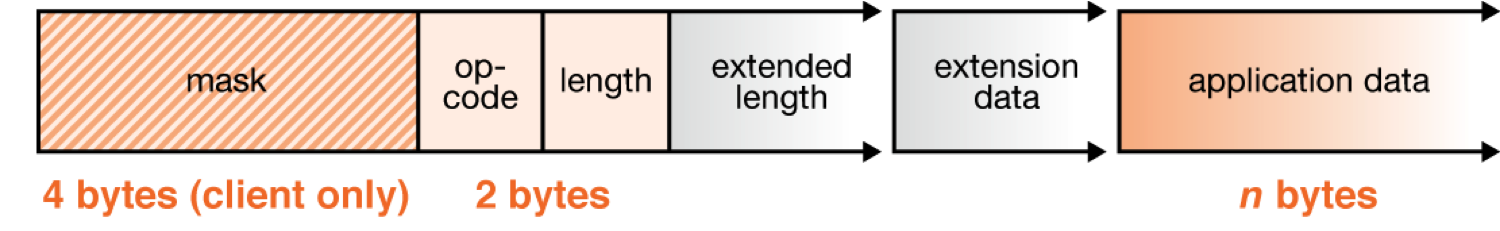
\includegraphics[height=0.9in,width=5.5in]{./images/websockets/WebSocketFrame.png}  
\caption{\small \sl The Websocket frame \label{fig:websocket_frame}}
\end{figure}

\begin{figure}
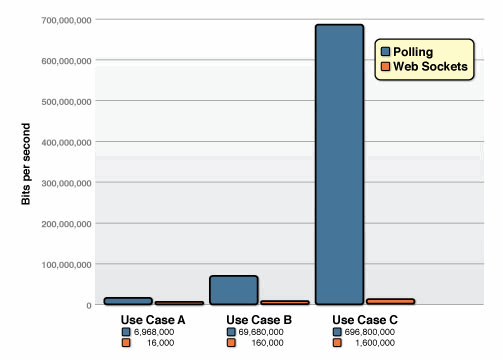
\includegraphics[height=3.94in,width=5.5in]{./images/websockets/poll-ws-compare.png}
\caption{\small \sl Websocket vs. HTTP Polling
\label{fig:websocket_ws_vs_polling}}
\end{figure}

After some further searching on the web, a forum answer\cite{websockets3} by the
founder of Tavendo, which develops Autobahn - A well-known set of Websocket libraries for
Javascript, Python and Android:\newline

\begin{quotation}
On a LAN, you can get Round-trip times for messages over WebSocket of 200
microseconds (from browser JS to WebSocket server and back), which is similar to
raw ICMP pings. On MAN, it's around 10ms, WAN (over residential ADSL to server in
same country) around 30ms, and so on up to around 120-200ms via 3.5G. The point
is: WebSocket does add virtually no latency to the one you will get anyway,
based on the network.\newline

The wire level overhead of WebSocket (compared to raw TCP) is between 2 octets
(unmasked payload of length < 126 octets) and 14 octets (masked payload of
length > 64k) per message (the former numbers assume the message is not
fragmented into multiple WebSocket frames). Very low.\newline

More so: with a WebSocket implementation capable of streaming processing, you
can (after the initial WebSocket handshake), start a single WebSocket message
and frame in each direction and then send up to 2\^63 octets with no overhead at
all. Essentially this renders WebSocket a fancy prelude for raw TCP. Caveat:
intermediaries may fragment the traffic at their own decision. However, if you
run WSS (that is secure WS = TLS), no intermediaries can interfere, and there
you are: raw TCP, with a HTTP compatible prelude (WS handshake).
\end{quotation}

This answer deems Websockets a fast protocol, appropriate for fast-paced games
such as the one described in this paper.\newline

Moreover, Websockets is designed with security standards and easy development in
mind. It has built - in connection management mechanisms that would easily fit
further development of this application. It would be basically eliminating
potential huge amounts of planning and development overhead induced by starting
a proprietary implementation on top of TCP. \newline

\appendix{Jackson vs. Gson}

When a choice had to be made for the JSON parsing library for this project, two
libraries came to mind: Jackson and GSON.\newline

Jackson is a project started in 2008 by Tatu Saloranta and Paul Brown. It has
gained popularity for it's features and fast serialization and deserialization
times.\newline

GSON is a project started in 2008 by Google. It has always been in direct
competition both for features and speed with Jackson.\newline

Some searches have been made for benchmarks for the two libraries. A few
blogs\cite{jacksonvsgson} \cite{jacksonvsgson2} \cite{jacksonvsgson4} and the
wiki entries for a few benchmarking tools\cite{jacksonvsgson3} \cite{jacksonvsgson5}
have been used as guidelines. The author has also tried out and weighted his
subjective opinion on the use of both libraries for simple serializing and
deserializing of JSON messages. The conclusions are as follows:
\begin{enumerate}
  \item \textbf{Features} - Although for the specific needs of this project,
  advanced features were not necessary, this criteria has been considered. A
  six part article on the blog programmerbruce.blogspot.de compares the features
  of GSON and Jackson and deems Jackson the better library.
  
  \item \textbf{Speed} - A test done in 2009 by Tatu Saloranta on his blog
  \url{http://www.cowtowncoder.com/blog/archives/2009/09/entry_326.html}, one of
  the two who started the Jackson project, deemed it much faster than GSON, as
  seen in Figure\ref{fig:jacksonvsgson1}. 'Tps' is \begin{quote}number of
  documents read, written, or read-modify-written per second\end{quote}
   
  \begin{figure}
  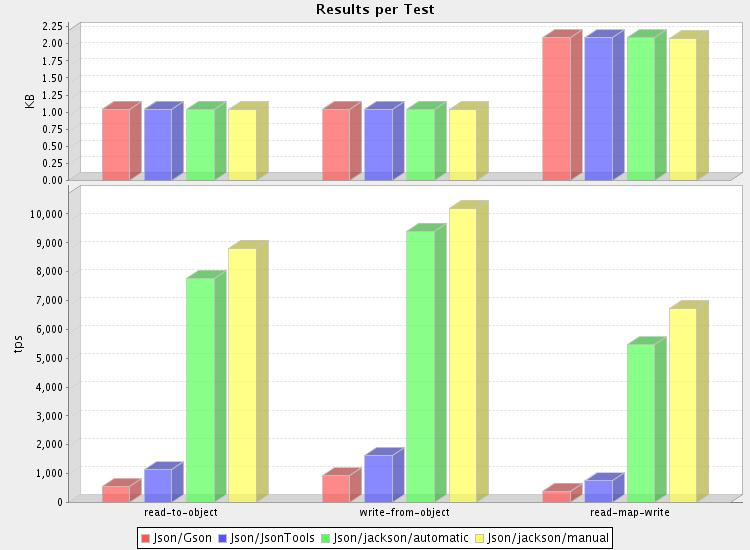
\includegraphics[height=3.5in,width=6.23in]{./images/benchmarks/testcase0.jpg}
  \caption{\small \sl Jackson vs Google-gson vs BerliOS
  (\textbf{\url{http://www.cowtowncoder.com/perf/json-bind-2009-09-23/testcase0.jpg}})}
  \label{fig:jacksonvsgson1}
  \end{figure}
  
  Another test has been done and published in a wiki entry of json-benchmark,
  in 2011. Android's Dalvik's ParseBenchmark.java has been used to benchmark
  the libraries. The results yielded have been:\newline
  \begin{verbatim}
                          TWEETS                              
           api run   ms linear runtime                    % 
ANDROID_STREAM   B 28.8 =================              207% 
JACKSON_STREAM   B 13.9 ========                       100% 
   GSON_STREAM   B 33.1 ===================            238% 
      ORG_JSON   B 36.2 =====================          260% 
     JSON_MINI   B 50.0 ============================== 360% 

                         READER_SHORT                        
           api run    ms linear runtime                    % 
ANDROID_STREAM   B  6.78 ================               177% 
JACKSON_STREAM   B  3.82 =========                      100% 
   GSON_STREAM   B  7.07 ================               185% 
      ORG_JSON   B  7.61 ==================             199% 
     JSON_MINI   B 12.49 ============================== 327% 

                        READER_LONG                         
           api run   ms linear runtime                    % 
ANDROID_STREAM   B 69.6 =====================          254% 
JACKSON_STREAM   B 27.4 ========                       100% 
   GSON_STREAM   B 68.1 =====================          248% 
      ORG_JSON   B 68.9 =====================          251% 
     JSON_MINI   B 95.0 ============================== 347% 
  \end{verbatim}  -
  \textbf{\url{https://code.google.com/p/json-benchmark/wiki/AndroidBenchmarks}}\newline
   
  A third test done in 2012 has been found on \url{blog.novoj.net}, where a
  multitude of libraries including Jackson 2.0.4 and GSON 2.1 were tested. This
  test also deems Jackson as faster at serializing/deserializing, as seen in
  Figure\ref{fig:jacksonvsgson2}.\newline
  
  \begin{figure}
  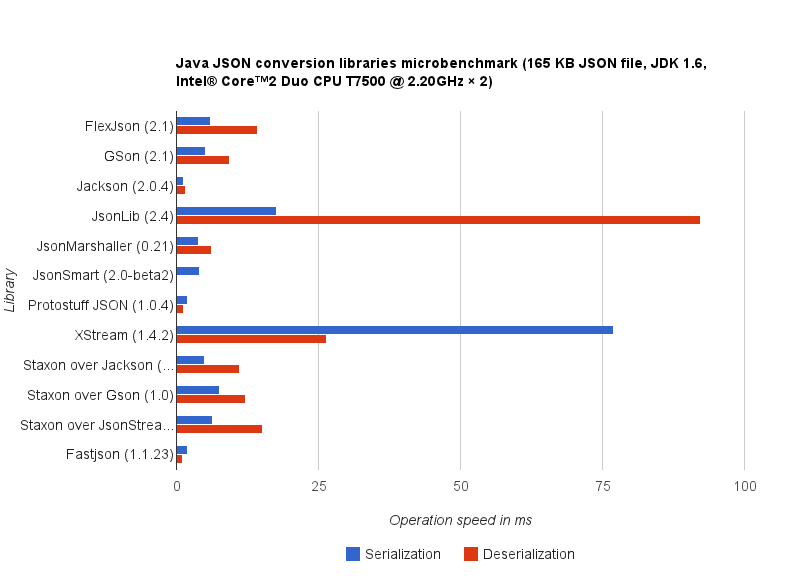
\includegraphics[height=4in,width=6.23in]{./images/benchmarks/oimg.png}
  \caption{\small \sl Jackson vs GSON in a comparison over multiple libraries
  (\textbf{\url{http://blog.novoj.net/2012/02/05/json-java-parsers-generators-microbenchmark/}})}
  \label{fig:jacksonvsgson2}
  \end{figure}
  
  A fourth test over several features of multiple JSON libraries, found in a
  wiki entry of jvm-serializers that has been last updated in 2013, also deems
  Jackson the fastest.
  
  \item \textbf{Personal choice} Both Jackson and GSON have been tried out
  before choosing one. Jackson has been preferred for it's ease of use and the fact
  that it offers the ObjectMapper, which gives straightforward functionality to
  'peel' layers from the JSON into Java HashMaps. GSON only allows the use of
  POJOs. For a project where changes have occurred often, like the one
  documented in this paper, Jackson was preferred.
  
  
\end{enumerate}


\appendix{Overlay tutorial}

This tutorial is for use with Google Maps V1 API. Recently, the Maps V1 API has
been deprecated and replaced with V2. Still, some who still have acquired keys
before the change can still use them until they expire. Otherwise, it
may be useful in other similar scenarios, where onTap functionality
has to be custom made.\newline
\begin{verbatim}

private UUID getClosestPlayerUUIDWithinTapRadius(GeoPoint geoPoint,
												 Double newTouchRadius){
		
		double touchRadius = 0.2; //expressed in inches
		
		if(newTouchRadius != null) touchRadius = newTouchRadius;		 
				
		double maximumAcceptedDistance = 
								calculateMaximumAcceptedDistance(touchRadius);
		
		Point touchScreenPoint = 
					MapUtils.convertGeoPointToScreenPoint(geoPoint, mapView);
		
		//get the closest point UUID and the closest distance
		UUID closestPointUUID = null;
		double closestPointDistance = Double.MAX_VALUE;
			
		
		Iterator iter = drawnPoints.entrySet().iterator();
		while(iter.hasNext()){			
			Entry<UUID, Point> entry = (Entry<UUID, Point>) iter.next();
			
			UUID uuid = entry.getKey();
			Point point = entry.getValue();
			
			double distance = 
					MapUtils.getDistanceBetweenPoints(point, touchScreenPoint);
			
			if(distance < closestPointDistance){
				closestPointDistance = distance;
				closestPointUUID = uuid;		
			}
		}
		
		if(touchRadius == Double.MAX_VALUE) 
			return closestPointUUID;
		
		else if(closestPointDistance <= maximumAcceptedDistance){
			return closestPointUUID;
		}
		
		
		return null;
		
	}
	
\end{verbatim}


\section{Countdown buttons Tutorial}

This tutorial is for adding dynamic countdowns for the elements in a Spinner
object. In the particular case of this application, the countdown is activated
based when the 'Shoot' button is pressed.\newline
\begin{enumerate}
  \item \textbf{Somewhere in the code, a ThreadPoolExecutor has to be created}:
  
\begin{verbatim}

private static final BlockingQueue<Runnable> workQueue = 
										new LinkedBlockingQueue<Runnable>(10);
ThreadPoolExecutor executor = 
				new ThreadPoolExecutor(3, 10, 3, TimeUnit.SECONDS, workQueue);
\end{verbatim}
	
  \item \textbf{Then, we define the class that implements Runnable. We will call
  it WeaponReportingTask}:

\begin{verbatim}
public class WeaponReportingTask extends AsyncTask<Weapon, Integer, Integer> {	
  		
	private boolean hasFinished = true;
	
	ArrayList<String> weaponsArray = null;
	ArrayAdapter<String> dataAdapter = null;
	int selectedIndex = 0;
	String initialWeaponName = "";	
	
	public WeaponReportingTask(
						ArrayList<String> newWeaponsArray, 
						ArrayAdapter<String> newDataAdapter,
						int newSelectedIndex
						){		
		super();
		
		hasFinished = true;
		
		weaponsArray = newWeaponsArray;
		dataAdapter = newDataAdapter;
		selectedIndex = newSelectedIndex;
		
		initialWeaponName = weaponsArray.get(selectedIndex);
	}
	
	

	@Override
 	protected Integer doInBackground(Weapon... params) {
	
		hasFinished = false;
		
		Weapon weapon = params[0];
 		if(weapon.getLastUsed() == null) 
 			return 0;
 		
 		int secondsElapsed = 
 					(int) MapUtils.getTimeDelta(weapon.getLastUsed(), true);
 		
 		while(secondsElapsed <= weapon.cooldown){
 			
 			publishProgress(weapon.cooldown - secondsElapsed);
 			
 			try {
				Thread.sleep(200);
			} catch (InterruptedException e) {
				// TODO Auto-generated catch block
				e.printStackTrace();
			}
 			
 			secondsElapsed = 
 					(int) MapUtils.getTimeDelta(weapon.getLastUsed(), true);
 		}
 		
 		return 1;
 	}
     
    
    protected synchronized void onProgressUpdate(Integer... progress) {
    	
    	if(progress != null)
    		weaponsArray.set(
    			selectedIndex, 
    			initialWeaponName+" ("+progress[0].toString()+" )"
    			);
    	
    	else 
    		weaponsArray.set(
    			selectedIndex, 
    			initialWeaponName
    			);
    	
    	dataAdapter.notifyDataSetChanged();
    }

    
    @Override
    protected void onPostExecute(Integer result) {
    	weaponsArray.set(selectedIndex, initialWeaponName);
    	dataAdapter.notifyDataSetChanged();    	
    	super.onPostExecute(result);
    	
    	hasFinished = true;
    	
    }
    
    @Override
    protected void onCancelled() {
    	weaponsArray.set(selectedIndex, initialWeaponName);
    	dataAdapter.notifyDataSetChanged();
    	super.onCancelled();
    	
    	hasFinished = true;
    }



	public boolean hasFinished() {
		return hasFinished;
	}
    
}

\end{verbatim}

  \item \textbf{And then, on 'Shoot', we launch it}:

\begin{verbatim}
WeaponReportingTask cooldownTimer = 
					new WeaponReportingTask(
							weapons,
							(ArrayAdapter<String>)weaponSpinner.getAdapter(),
							currentWeaponIndex
							);
cooldownTimer.executeOnExecutor(
		executor,
		currentWeapon //this object is used in the WeaponReportingTask only  
					  //for the cooldown time specific to the Weapon object.
		);
\end{verbatim}


\end{enumerate}



\end{appendices}




%----------------------------------------------------------------------------------------
%	BIBLIOGRAPHY
%----------------------------------------------------------------------------------------





\section{Bibliography}
	\bibliographystyle{ieeetr}	
	\bibliography{bibcontent}




	
	
	
	
	
	\begin{verbatim}
	
	
	
	
	
	
	
	
	
	
	
	I, Vadim Costache, hereby declare that my Master Thesis was written	independently, 
	that none other than the specified sources and aids were used and that any
	citations have been marked.
	
	
	
	
	
	
	
	
	
	
	
	
	
	
	
	Vadim Costache

	
	
	
	
	
	
	
	
	
	
	
	
	
	
	
	\end{verbatim}

\end{document}





















